% Options for packages loaded elsewhere
\PassOptionsToPackage{unicode}{hyperref}
\PassOptionsToPackage{hyphens}{url}
\documentclass[
]{book}
\usepackage{xcolor}
\usepackage{amsmath,amssymb}
\setcounter{secnumdepth}{5}
\usepackage{iftex}
\ifPDFTeX
  \usepackage[T1]{fontenc}
  \usepackage[utf8]{inputenc}
  \usepackage{textcomp} % provide euro and other symbols
\else % if luatex or xetex
  \usepackage{unicode-math} % this also loads fontspec
  \defaultfontfeatures{Scale=MatchLowercase}
  \defaultfontfeatures[\rmfamily]{Ligatures=TeX,Scale=1}
\fi
\usepackage{lmodern}
\ifPDFTeX\else
  % xetex/luatex font selection
\fi
% Use upquote if available, for straight quotes in verbatim environments
\IfFileExists{upquote.sty}{\usepackage{upquote}}{}
\IfFileExists{microtype.sty}{% use microtype if available
  \usepackage[]{microtype}
  \UseMicrotypeSet[protrusion]{basicmath} % disable protrusion for tt fonts
}{}
\makeatletter
\@ifundefined{KOMAClassName}{% if non-KOMA class
  \IfFileExists{parskip.sty}{%
    \usepackage{parskip}
  }{% else
    \setlength{\parindent}{0pt}
    \setlength{\parskip}{6pt plus 2pt minus 1pt}}
}{% if KOMA class
  \KOMAoptions{parskip=half}}
\makeatother
\usepackage{color}
\usepackage{fancyvrb}
\newcommand{\VerbBar}{|}
\newcommand{\VERB}{\Verb[commandchars=\\\{\}]}
\DefineVerbatimEnvironment{Highlighting}{Verbatim}{commandchars=\\\{\}}
% Add ',fontsize=\small' for more characters per line
\usepackage{framed}
\definecolor{shadecolor}{RGB}{248,248,248}
\newenvironment{Shaded}{\begin{snugshade}}{\end{snugshade}}
\newcommand{\AlertTok}[1]{\textcolor[rgb]{0.94,0.16,0.16}{#1}}
\newcommand{\AnnotationTok}[1]{\textcolor[rgb]{0.56,0.35,0.01}{\textbf{\textit{#1}}}}
\newcommand{\AttributeTok}[1]{\textcolor[rgb]{0.13,0.29,0.53}{#1}}
\newcommand{\BaseNTok}[1]{\textcolor[rgb]{0.00,0.00,0.81}{#1}}
\newcommand{\BuiltInTok}[1]{#1}
\newcommand{\CharTok}[1]{\textcolor[rgb]{0.31,0.60,0.02}{#1}}
\newcommand{\CommentTok}[1]{\textcolor[rgb]{0.56,0.35,0.01}{\textit{#1}}}
\newcommand{\CommentVarTok}[1]{\textcolor[rgb]{0.56,0.35,0.01}{\textbf{\textit{#1}}}}
\newcommand{\ConstantTok}[1]{\textcolor[rgb]{0.56,0.35,0.01}{#1}}
\newcommand{\ControlFlowTok}[1]{\textcolor[rgb]{0.13,0.29,0.53}{\textbf{#1}}}
\newcommand{\DataTypeTok}[1]{\textcolor[rgb]{0.13,0.29,0.53}{#1}}
\newcommand{\DecValTok}[1]{\textcolor[rgb]{0.00,0.00,0.81}{#1}}
\newcommand{\DocumentationTok}[1]{\textcolor[rgb]{0.56,0.35,0.01}{\textbf{\textit{#1}}}}
\newcommand{\ErrorTok}[1]{\textcolor[rgb]{0.64,0.00,0.00}{\textbf{#1}}}
\newcommand{\ExtensionTok}[1]{#1}
\newcommand{\FloatTok}[1]{\textcolor[rgb]{0.00,0.00,0.81}{#1}}
\newcommand{\FunctionTok}[1]{\textcolor[rgb]{0.13,0.29,0.53}{\textbf{#1}}}
\newcommand{\ImportTok}[1]{#1}
\newcommand{\InformationTok}[1]{\textcolor[rgb]{0.56,0.35,0.01}{\textbf{\textit{#1}}}}
\newcommand{\KeywordTok}[1]{\textcolor[rgb]{0.13,0.29,0.53}{\textbf{#1}}}
\newcommand{\NormalTok}[1]{#1}
\newcommand{\OperatorTok}[1]{\textcolor[rgb]{0.81,0.36,0.00}{\textbf{#1}}}
\newcommand{\OtherTok}[1]{\textcolor[rgb]{0.56,0.35,0.01}{#1}}
\newcommand{\PreprocessorTok}[1]{\textcolor[rgb]{0.56,0.35,0.01}{\textit{#1}}}
\newcommand{\RegionMarkerTok}[1]{#1}
\newcommand{\SpecialCharTok}[1]{\textcolor[rgb]{0.81,0.36,0.00}{\textbf{#1}}}
\newcommand{\SpecialStringTok}[1]{\textcolor[rgb]{0.31,0.60,0.02}{#1}}
\newcommand{\StringTok}[1]{\textcolor[rgb]{0.31,0.60,0.02}{#1}}
\newcommand{\VariableTok}[1]{\textcolor[rgb]{0.00,0.00,0.00}{#1}}
\newcommand{\VerbatimStringTok}[1]{\textcolor[rgb]{0.31,0.60,0.02}{#1}}
\newcommand{\WarningTok}[1]{\textcolor[rgb]{0.56,0.35,0.01}{\textbf{\textit{#1}}}}
\usepackage{longtable,booktabs,array}
\usepackage{calc} % for calculating minipage widths
% Correct order of tables after \paragraph or \subparagraph
\usepackage{etoolbox}
\makeatletter
\patchcmd\longtable{\par}{\if@noskipsec\mbox{}\fi\par}{}{}
\makeatother
% Allow footnotes in longtable head/foot
\IfFileExists{footnotehyper.sty}{\usepackage{footnotehyper}}{\usepackage{footnote}}
\makesavenoteenv{longtable}
\usepackage{graphicx}
\makeatletter
\newsavebox\pandoc@box
\newcommand*\pandocbounded[1]{% scales image to fit in text height/width
  \sbox\pandoc@box{#1}%
  \Gscale@div\@tempa{\textheight}{\dimexpr\ht\pandoc@box+\dp\pandoc@box\relax}%
  \Gscale@div\@tempb{\linewidth}{\wd\pandoc@box}%
  \ifdim\@tempb\p@<\@tempa\p@\let\@tempa\@tempb\fi% select the smaller of both
  \ifdim\@tempa\p@<\p@\scalebox{\@tempa}{\usebox\pandoc@box}%
  \else\usebox{\pandoc@box}%
  \fi%
}
% Set default figure placement to htbp
\def\fps@figure{htbp}
\makeatother
\setlength{\emergencystretch}{3em} % prevent overfull lines
\providecommand{\tightlist}{%
  \setlength{\itemsep}{0pt}\setlength{\parskip}{0pt}}
\usepackage[]{natbib}
\bibliographystyle{plainnat}
\usepackage{booktabs}

\AtBeginEnvironment{verbatim}{\small}
\AtEndEnvironment{verbatim}{}

%\usepackage{fontsize}
%\newcommand{\codefont}{\fontsize{8pt}{10pt}\selectfont}
%\renewcommand{\VerbatimFont}[1]{\fontsize{8pt}{10pt}\selectfont}

%\usepackage{titlesec}
%\newcommand{\sectionbreak}{\clearpage}
%, provide=*
\usepackage[estonian, provide=*]{babel}
\usepackage{float}

\usepackage{CormorantGaramond}
\usepackage{ebgaramond-maths}
%\usepackage{times}

\usepackage{makeidx}


\usepackage[top=25mm,
   bottom=25mm,
   inner=25mm,
   outer=20mm]{geometry}

\usepackage[labelsep=period,small,singlelinecheck=false]{caption}

\usepackage{fancyhdr}

\setlength{\headheight}{15pt}
\fancypagestyle{plain}{%
	\fancyhf{} % eemalda kõik päised ja jalused
	\renewcommand{\headrulewidth}{0pt} % eemalda joon päise all
	\fancyfoot[C]{\thepage} % ainult lehekülje number
}
\pagestyle{fancy}
\fancyhf{}
\fancyhead[LE,RO]{\thepage}
\fancyhead[RE]{\leftmark}
\fancyhead[LO]{\rightmark}

   
% Kaane kujunduse määratlus
\usepackage{graphicx} % Vajalik piltide lisamiseks
\usepackage[absolute,overlay]{textpos} % Teksti paigutamiseks pildi peale
\usepackage{xcolor} % Värvi kasutamiseks

\DefineVerbatimEnvironment{naideExcel}{Verbatim}{
	xleftmargin=.5cm,
	fontsize=\small,
	formatcom=\color{blue},
	baselinestretch=0.9,
	fontfamily=cmtt
}


\renewcommand{\normalsize}{\fontsize{12}{18}\selectfont}


%\RecustomVerbatimEnvironment{Highlighting}{Verbatim}{fontsize=\small}
\renewenvironment{Shaded} {\begin{snugshade}\footnotesize} {\end{snugshade}}
% Kaane lehe määratlus
\newcommand{\kaanekaas}{
    \begin{titlepage} % Alustab kaane lehte
    \begin{center}
        \vspace*{5cm} % Lisab vertikaalset ruumi

        % Raamatu pealkiri
        {\Huge\bfseries Metsanduslik statistika }\\
        \vspace{0.5cm}
        
        % Alapealkiri
        {\Large R ja MS Excel keskkonnas}\\
        \vspace{3cm}
        
        % Autor
        {\Large\textit{Allan Sims}}\\
        \vspace{0.5cm}
        {\Large\textit{Andres Kiviste}}\\
        \vspace{0.5cm}
        {\Large\textit{Diana Laarmann}}\\
        \vspace{1cm}
        
        % Kaanepilt
        %\includegraphics[width=\textwidth]{kaanepilt.jpg}\\
        %\vspace{2cm}
        
        % Avaldamise kuupäev või muu tekst
        %{\Large 2024}
        
        \vfill
        
        % Kirjastuse või muu asjakohase info lisamine
        {\large 2025}
        
    \end{center}
    \end{titlepage}
}

% Kaane lehe lisamine dokumenti enne sisu algust
%\AtBeginDocument{\kaanekaas}
   
\usepackage{bookmark}
\IfFileExists{xurl.sty}{\usepackage{xurl}}{} % add URL line breaks if available
\urlstyle{same}
\hypersetup{
  pdftitle={Metsanduslik statistika R ja MS Excel keskkonnas},
  pdfauthor={Allan Sims, Andres Kiviste, Diana Laarmann},
  hidelinks,
  pdfcreator={LaTeX via pandoc}}

\title{Metsanduslik statistika R ja MS Excel keskkonnas}
\author{Allan Sims, Andres Kiviste, Diana Laarmann}
\date{31.01.2025}

\begin{document}
\maketitle

{
\setcounter{tocdepth}{1}
\tableofcontents
}
\chapter{Sissejuhatus}\label{sissejuhatus}

Käesolev õpik on mõeldud metsandusüliõpilastele, kes soovivad omandada matemaatilise statistika põhitõdesid praktilises kontekstis. Materjali koostamisel on lähtutud eeldusest, et lugejatel ei pruugi olla sügavamat matemaatilist ettevalmistust. Terminoloogia on kooskõlas ``Andmeanalüüsi ja statistika oskussõnastikuga'' (\url{https://sonaveeb.ee/ds/aso}), kuid mõisted on lahtiseletatud metsandusvaldkonnast lähtuvalt.

Metsanduses toimub pidev andmete kogumine ja nende töötlemine. Kõiki soovitud andmeid ei ole võimalik alati mõõta ning seetõttu tuletatakse need erinevate mudelite abil. Sellised mudelid on saadud statistilise andmetöötluse ja modelleerimise abil. Seetõttu on andmete töötlemisel oluline tunda ka statistika põhitõdesid, et mõista paremini andmetest järelduste ja otsuste tegemisel. Õpiku näited keskenduvad metsanduslikele andmetele. Tarkvarana on kasutatud statistikatarkvara \textbf{R} ja \textbf{MS Excel}, kuid nende valikul on oluline märkida nende erinevaid võimekusi:

\begin{enumerate}
\def\labelenumi{\arabic{enumi}.}
\tightlist
\item
  \textbf{R} on spetsialiseerunud statistiliseks modelleerimiseks ja analüüsiks, pakkudes laia valikut meetodeid (nt regressioon, testid). Kuid andmehalduse lihtsustamiseks võib olla vaja täiendavaid tööriistu.\\
\item
  \textbf{MS Excel} on kasutajasõbralik platvorm andmete korrastamiseks ja esmaseks visualiseerimiseks, kuid selle statistilised funktsioonid on piiratud (nt puuduvad keerukama modelleerimise võimalused).
\end{enumerate}

Need tarkvarad täiendavad üksteist. MS Excel sobib hästi andmete esmaseks töötluseks, R aga detailsemaks analüüsiks. Näiteks võib MS Excelis ette valmistatud andmeid edasi analüüsida R-is. Samuti on võimalik integreerida R-skripte Exceli makrotesse või kasutada Pythoni skripte R-i keskkonnas, et laiendada funktsionaalsust, aga neid integratsioone käesolev õpik ei käsitle. Sellised moodulipõhised lahendused muudavad tarkvaravahendid paindlikumaks, kuid nõuavad aga pidevat oskuste arendamist.

Oluline on mõista, et üksik tarkvara ei suuda katta kõiki analüüsivajadusi. Seetõttu on õpikus rõhk praktilistel lahendustel, mis õpetavad ülesannete jaoks optimaalsete tööriistade valikut. Statistika valdkond areneb kiiresti -- nii meetodid, tarkvarad kui rakendusvaldkonnad muutuvad. Käesolevat õpikut uuendatakse regulaarselt, et kajastada ajakohaseid standardeid ja tarkvarauuendusi.

\section{Statistikaprogramm R}\label{statistikaprogramm-r}

R on tarkvarakeskkond, mis on loodud spetsiaalselt statistiliseks arvutamiseks ja andmete graafiliseks esitamiseks. See on avatud lähtekoodiga projekt, mida toetab suur kogukond ning mida eelistavad andmeteadlased ja statistikud üle kogu maailma oma andmeanalüüsi vajadusteks. R pakub laia valikut tööriistu andmete importimiseks, töötlemiseks, modelleerimiseks, analüüsiks ja visualiseerimiseks. Järgnevalt on ülevaade R-i peamistest kasutusvõimalustest statistilise analüüsi tegemiseks.

\textbf{Andmete importimine ja töötlemine}

\begin{itemize}
\tightlist
\item
  \textbf{Andmete importimine.} R toetab andmete importimist paljudest allikatest, sealhulgas teksti-, CSV- ja MS Exceli failidest ning andmebaasidest ja isegi veebist.
\item
  \textbf{Andmete puhastamine.} Andmete analüüsiks ettevalmistamisel pakub R võimalusi nende sortimiseks, filtreerimiseks, puuduvate väärtuste käsitlemiseks ja duplikaatide eemaldamiseks.
\end{itemize}

\textbf{Andmete analüüs}

\begin{itemize}
\tightlist
\item
  \textbf{Statistilised funktsioonid.} R sisaldab ulatuslikku valikut sisseehitatud funktsioone statistilisi tunnuste arvutamiseks, nagu keskmine, mediaan, standardhälve, kvantiilid ja palju muud, mis võimaldavad kiiresti arvutada olulisi statistilisi näitajaid.
\item
  \textbf{Andmete manipuleerimine.} R pakub võimekaid pakette andmete manipuleerimiseks, mis võimaldavad efektiivselt andmete filtreerimist, valimist, rühmitamist ja kokkuvõtete tegemist.
\end{itemize}

\textbf{Statistilised mudelid ja analüüsimeetodid}

\begin{itemize}
\tightlist
\item
  \textbf{Hüpoteeside testimine.} R võimaldab kasutajatel teostada erinevaid statistilisi teste, nagu t-testid, hii-ruut-testid, ANOVA ja palju muud, et uurida andmete omavahelisi seoseid ja testida hüpoteese.
\item
  \textbf{Regressioon ja korrelatsioon.} R toetab mitmesuguseid regressioonianalüüse võimaldades seeläbi uurida muutujate vahelisi seoseid.
\end{itemize}

\textbf{Andmete visualiseerimine}

\begin{itemize}
\tightlist
\item
  \textbf{Graafikud ja diagrammid.} R pakub mitmeid pakette andmete visualiseerimiseks võimaldades luua keerukaid ja esteetiliselt meeldivaid graafikuid.
\item
  \textbf{Interaktiivsed visualisatsioonid.} Lisaks staatilistele graafikutele võimaldab R luua interaktiivseid visualisatsioone.
\end{itemize}

\textbf{Laiendatavus ja kogukond}

\begin{itemize}
\tightlist
\item
  \textbf{Pakettide ökosüsteem.} R toetab laialdast pakettide ökosüsteemi, mis katab spetsiifilisi statistilisi meetodeid, andmete visualiseerimise tehnikaid, masinõpet ja palju muud, võimaldades kasutajatel laiendada R-i funktsionaalsust vastavalt vajadusele.
\item
  \textbf{Tugev kogukond.} R-i kasutajate ja arendajate kogukond on väga aktiivne, pakkudes tuge, juhendeid ja ressursse, mis aitavad lahendada keerulisi analüütilisi väljakutseid.
\item
  \textbf{Õpikud ja juhendid.} R-i kasutamiseks on koostatud erinevaid õpikud, mis on mõeldud nii algajatele kui ka edasijõudnutele. Veebilehel \url{https://bookdown.org/} on mitmed sellised õpikud.
\end{itemize}

\subsection{R-i paketid}\label{r-i-paketid}

Statistikaprogramm põhineb pakettidel. Iga pakett on meetodite ja funktsioonide kogumik ning need võimaldavad teha kindlaid protseduure. Kasutajal on võimalik installeerida teiste poolt koostatud pakette või neid vajadusel ise koostada. R-i paketid on tööriistade, funktsioonide ja andmete kogumikud, mis laiendavad R-i põhifunktsionaalsust ning võimaldavad lahendada erinevaid andmetöötluse, statistilise analüüsi ja visualiseerimise ülesandeid. Enamik pakette on loodud R-i kogukonna liikmete poolt. CRAN (Comprehensive R Archive Network) on ametlik hoidla, kuhu arendajad saavad pakette üles laadida ning kasutajad neid alla laadida.

Pakettide installeerimiseks kasutatakse funktsiooni \texttt{install.packages()}. Näiteks:

\begin{Shaded}
\begin{Highlighting}[]
\FunctionTok{install.packages}\NormalTok{(}\StringTok{"ggplot2"}\NormalTok{)}
\end{Highlighting}
\end{Shaded}

Kui pakett on installitud, tuleb see sessioonis laadida, kasutades funktsiooni \texttt{library()}:

\begin{Shaded}
\begin{Highlighting}[]
\FunctionTok{library}\NormalTok{(ggplot2) }
\CommentTok{\# või}
\FunctionTok{library}\NormalTok{(}\StringTok{"ggplot2"}\NormalTok{)}
\end{Highlighting}
\end{Shaded}

Pakettide puhul tuleb jälgida, et installimise funktsioonis peab paketi nimetus olema jutumärkide vahel, aga paketi sisse laadimisel võib see olla ka jutumärkideta.

Lisaks on ka funktsioon \texttt{require()}, mis võimaldab testida paketi olemasolu. Selline testimise vajadus tekib, kui skripti kasutatakse korduvalt erinevates arvutites ning ühes arvutis skripti loomisel võib olla vajalikud paketid juba installitud ning teises arvutis ei pruugi veel vajalikke pakette olla. Näiteks, kontrollime, kas antud pakett on olemas ning kui see puudub, siis installime:

\begin{Shaded}
\begin{Highlighting}[]
\ControlFlowTok{if}\NormalTok{(}\SpecialCharTok{!}\FunctionTok{require}\NormalTok{(ggplot2))\{}
    \FunctionTok{install.packages}\NormalTok{(}\StringTok{"ggplot2"}\NormalTok{)    }
\NormalTok{\}}
\end{Highlighting}
\end{Shaded}

Funktsioon \texttt{require()} loeb ka paketi sisse, kui see on installitud, aga seda on soovituslik kasutada pigem selleks, et kontrollida paketi olemasolu. Kui koostatud on arvutusskript, milles antud funktsiooniga laaditakse pakett, mis puudub, siis skripti töö jätkub, aga see ebaõnnestub, sest vajalikku paketti ei ole.

Igal paketil on põhjalik dokumentatsioon, millele pääseb ligi, kasutades \texttt{help()} või \texttt{?} süntaksit. Paljud paketid pakuvad ka sissejuhatavaid õpetusi ja veebipõhiseid juhendeid.

\section{MS Excel}\label{ms-excel}

MS Excel on laialdaselt kasutatav tabelarvutusprogramm, mis pakub mitmekülgseid tööriistu andmete analüüsimiseks, visualiseerimiseks ja esitlemiseks. MS Exceli kasutusvõimalused statistilise analüüsi tegemiseks hõlmavad mitmesuguseid funktsioone ja lisavahendeid, mis võimaldavad kasutajatel teostada põhjalikke analüüse erinevate andmekogumite põhjal. Järgnevalt on toodud ülevaade peamistest MS Exceli kasutusvõimalustest statistiliseks analüüsiks.

\textbf{Andmete importimine ja korraldamine}

\begin{itemize}
\tightlist
\item
  \textbf{Andmete importimine.} Excel võimaldab importida andmeid erinevatest allikatest, sealhulgas tekstifailidest, CSV-failidest, andmebaasidest ja veebiteenustest.
\item
  \textbf{Andmete puhastamine ja ettevalmistamine.} Kasutajad saavad kasutada tööriistu, nagu sortimine, filtreerimine ja eemaldamine, et korrastada andmeid analüüsi jaoks. Samuti on võimalik kasutada tingimusvormingut, et esile tõsta olulisi andmepunkte või mustreid.
\end{itemize}

\textbf{Andmete analüüsimine}

\begin{itemize}
\tightlist
\item
  \textbf{Põhilised statistilised funktsioonid.} Excel sisaldab mitmesuguseid statistilisi funktsioone, nagu keskmine (AVERAGE), mediaan (MEDIAN), standardhälve (STDEV), minimaalne (MIN) ja maksimaalne (MAX) väärtus.
\item
  \textbf{Liigendtabelid.} Liigendtabelid võimaldavad kiiresti kokku võtta, analüüsida, uurida ja esitada andmeid. Kasutajad saavad hõlpsasti grupeerida ja segmenteerida andmeid, et tuvastada mustreid või suundumusi.
\end{itemize}

\textbf{Statistilised testid ja analüüsimeetodid}

\begin{itemize}
\tightlist
\item
  \textbf{Hüpoteeside testimine.} Excelis saab teostada t-Testi ja ANOVA (Analysis of Variance) teste, et võrrelda andmekogumeid või analüüsida erinevusi rühmade vahel.
\item
  \textbf{Regressioonianalüüs.} Kasutajad saavad kasutada regressioonianalüüsi, et uurida muutujate vahelisi seoseid ja ennustada tulemusi.
\end{itemize}

\textbf{Andmete visualiseerimine}
- \textbf{Diagrammid ja graafikud.} Excel pakub erinevaid viise andmete visualiseerimiseks, sealhulgas tulp-, joon-, piirkonna-, ring-, hajuvus- ja mullidiagramme.
- \textbf{Tingimuslik vormindamine:} See võimaldab andmeid visuaalselt esile tõsta, kasutades värve, ikoone ja andmeribasid, et lihtsustada andmestiku mustrite ja trendide tuvastamist.

\textbf{Makrod ja VBA skriptimine}
- \textbf{Automatiseerimine ja kohandamine.} Kasutajad saavad luua makrosid ja kasutada Visual Basic for Applications (VBA) skriptimist, et automatiseerida korduvaid ülesandeid ja kohandada analüütilisi protseduure, mis ületavad Exceli standardfunktsioonide piire.

\textbf{Lisandmoodulid ja tööriistad}
- \textbf{Analysis ToolPak.} See on MS Exceli lisandmoodul, mis pakub täiendavaid statistilisi funktsioone, sealhulgas keerulisemaid analüütilisi tööriistu ja statistilisi meetodeid.

MS Exceli paindlikkus ja lai funktsionaalsus muudavad selle heaks tööriistaks statistiliseks analüüsiks. Siiski on oluline märkida, et keerukamate statistiliste analüüside ja suurte andmekogumite korral pakuvad spetsialiseeritud statistikatarkvarad rohkem võimalusi.

\chapter{Andmestik}\label{andmestik}

Metsanduses kogutakse pidevalt mitmesuguseid andmeid, mis võivad erineda nii oma tüübilt kui ka struktuurilt. Andmekogumise protsessi üldnimetus on \textbf{takseerimine}, mis hõlmab mitmesuguseid meetodeid nagu mõõtmine, loendamine, määramine ja muud sarnased tegevused. Iga takseerimisviis määrab ühtlasi ka kogutavate andmete tüübi.

\begin{itemize}
\tightlist
\item
  \textbf{Mõõtmisel} saadakse enamasti \textbf{pidev tunnus}. See on tunnus, mille väärtused võivad olla mistahes arvud teatud vahemikus. See tähendab, et pideva tunnuse puhul ei ole väärtused piiratud kindlate, eraldiseisvate arvudega, vaid võivad muutuda sujuvalt ja pidevalt. Näiteks mõõdetud puu kõrgus või diameeter.
\item
  \textbf{Loendamisel} saadakse \textbf{diskreetne tunnus}. See on tunnus, mille väärtused saavad olla ainult teatud kindlad, eraldiseisvad arvud, tavaliselt täisarvud. See tähendab, et diskreetsete tunnuste puhul ei saa väärtused olla sujuvad või pidevad, vaid peavad olema selgelt eristuvad. Näiteks puude ja aastarõngaste loendamine. Diskreetne on ka rinnaspindala mõõtmisel relaskoobiga loendamine, kus loendatakse puid, kuid teatud juhtudel kasutatakse ka konstanti 0,5.
\item
  \textbf{Määramisel} saadakse üldjuhul \textbf{nominaalne tunnus}. See on selline tunnus, mis väljendab kvalitatiivseid ehk mittearvulisi andmeid, mida ei saa järjestada. Näiteks puuliik, kasvukohatüüp vms. Selle alla liigitub ka \textbf{ordinaalne tunnus} ehk järjestustunnus on tunnus, mille väärtustel on loogiline järjestus, kuid väärtuste vahed ei ole tingimata võrdsed. Näiteks on metsanduses selleks boniteediklass.
\end{itemize}

Statistikas tähendab \textbf{andmestik} vaatlusandmete kogumit, mis on kogutud mingi uuringu või eksperimendi käigus. See on toorandmete hulk, mida analüüsitakse, et avastada mustreid, seoseid ja teha järeldusi. Andmete tüüp mängib olulist rolli statistilises analüüsis, kuna see määrab, milliseid meetodeid ja visualiseerimisviise saab kasutada. Õige andmetüübi tuvastamine on seega esimene samm edukaks andmetöötluseks ja tulemuste tõlgendamiseks.

Andmestik on organiseeritud andmete kogum, mis on tavaliselt salvestatud tabelitesse, andmebaasidesse või muudesse struktuuridesse.

\begin{itemize}
\tightlist
\item
  \textbf{Tüübid:}

  \begin{itemize}
  \tightlist
  \item
    \textbf{Vektor:} Sama tüüpi väärtuste jada (nt arvude vektor, tekstiväärtuste vektor).
  \item
    \textbf{Maatriks:} Sama tüüpi väärtuste kogum, kuid mis on mitmemõõtmeline.
  \item
    \textbf{Andmetabel:} Struktureeritud andmete kogum, kus iga rida esindab ühte objekti ja iga veerg esindab objekti atribuuti.
  \end{itemize}
\end{itemize}

\section{Andmestiku struktuur R keskkonnas}\label{andmestiku-struktuur-r-keskkonnas}

\subsection{Vektor}\label{vektor}

Vektor on andmetüüp, mis võimaldab talletada mitut ühesugust andmetüüpi elementi ühes andmestruktuuris. Vektoris saab hoida näiteks numbreid, teksti või loogilisi väärtusi. Vektorit loetakse ühemõõtmeliseks andmestruktuuriks, kuna kõik selles sisalduvad elemendid asuvad ühes reas.

Vektorit saab luua kasutades funktsiooni \texttt{c()}, kuhu tuleb sisestada eraldatud komadega elemendid. Näiteks:

\begin{Shaded}
\begin{Highlighting}[]
\CommentTok{\# Näide R keskkonnas}

\NormalTok{num\_vektor }\OtherTok{\textless{}{-}} \FunctionTok{c}\NormalTok{(}\DecValTok{1}\NormalTok{, }\DecValTok{2}\NormalTok{, }\DecValTok{3}\NormalTok{, }\DecValTok{4}\NormalTok{, }\DecValTok{5}\NormalTok{)}
\end{Highlighting}
\end{Shaded}

Vektori elementidele saab viidata indeksite abil, alustades indeksist 1. Näiteks:

\begin{Shaded}
\begin{Highlighting}[]
\CommentTok{\# Näide R keskkonnas}

\CommentTok{\# väljastab vektori num\_vektor kolmanda elemendi väärtuse}
\NormalTok{num\_vektor[}\DecValTok{3}\NormalTok{] }
\end{Highlighting}
\end{Shaded}

\begin{verbatim}
[1] 3
\end{verbatim}

Vektori pikkus ehk elementide arv on võimalik saada funktsiooniga \texttt{length()}. Vektorit saab ühendada teise vektoriga funktsiooniga \texttt{c()}. Näiteks:

\begin{Shaded}
\begin{Highlighting}[]
\CommentTok{\# Näide R keskkonnas}

\NormalTok{num\_vektor\_2 }\OtherTok{\textless{}{-}} \FunctionTok{c}\NormalTok{(}\DecValTok{6}\NormalTok{, }\DecValTok{7}\NormalTok{, }\DecValTok{8}\NormalTok{)}
\NormalTok{kombineeritud\_vektor }\OtherTok{\textless{}{-}} \FunctionTok{c}\NormalTok{(num\_vektor, num\_vektor\_2)}
\end{Highlighting}
\end{Shaded}

Võimalik on ka vektorit luua jada genereerimise abil, kasutades funktsiooni \texttt{seq()}. Näiteks:

\begin{Shaded}
\begin{Highlighting}[]
\CommentTok{\# Näide R keskkonnas}

\CommentTok{\# loob vektori, mis sisaldab arve vahemikus 1 kuni 10 sammuga 2}
\NormalTok{jarg\_vector }\OtherTok{\textless{}{-}} \FunctionTok{seq}\NormalTok{(}\DecValTok{1}\NormalTok{, }\DecValTok{10}\NormalTok{, }\AttributeTok{by =} \DecValTok{2}\NormalTok{) }
\end{Highlighting}
\end{Shaded}

Vektoritega on võimalik teostada erinevaid arvutusi, teisendusi ning andmete filtreerimist. Vektorid on olulised R programmeerimises, kuna nende abil on mugav töödelda andmeid ja teostada statistilisi analüüse.

\subsection{Maatriks}\label{maatriks}

Andmetüüp maatriks on kahe- või mitmemõõtmeline andmete struktuur, kus andmed on paigutatud mitme rea ja veeruna, moodustades seeläbi mitmemõõtmelise andmestiku. Maatriksis olevad andmed peavad olema kõik samatüübilised, näiteks kõik arvud või kõik tekstid.

Maatriksi loomiseks kasutatakse funktsioone \texttt{matrix()} või \texttt{array()}, millest esimene võimaldab luua kahemõõtmelist ning teine juba mitmemõõtmelisi maatrikseid. Nendele funktsioonidele saab määrata erinevaid parameetreid, näiteks andmete sisu, ridade ja veergude arvu ning rea- ja veerunimed.

\begin{Shaded}
\begin{Highlighting}[]
\CommentTok{\# Näide R keskkonnas}
\CommentTok{\# funktsioon runif() loob juhuslike andmete vektori}
\CommentTok{\# Loome kahemõõtmelise maatriksi juhuslikest arvudest}
\NormalTok{minu\_maatriks }\OtherTok{\textless{}{-}} \FunctionTok{matrix}\NormalTok{(}\FunctionTok{runif}\NormalTok{(}\DecValTok{12}\NormalTok{), }\AttributeTok{nrow=}\DecValTok{3}\NormalTok{, }\AttributeTok{ncol=}\DecValTok{4}\NormalTok{)}
\FunctionTok{print}\NormalTok{(minu\_maatriks)}
\end{Highlighting}
\end{Shaded}

\begin{verbatim}
      [,1]  [,2]  [,3]  [,4]
[1,] 0,185 0,325 0,701 0,122
[2,] 0,141 0,476 0,770 0,459
[3,] 0,711 0,948 0,182 0,854
\end{verbatim}

\begin{Shaded}
\begin{Highlighting}[]
\CommentTok{\# Loome kolmemõõtmelise maatriksi juhuslikest arvudest}
\NormalTok{minu\_array }\OtherTok{\textless{}{-}} \FunctionTok{array}\NormalTok{(}\FunctionTok{runif}\NormalTok{(}\DecValTok{12}\NormalTok{), }\AttributeTok{dim =} \FunctionTok{c}\NormalTok{(}\DecValTok{2}\NormalTok{,}\DecValTok{2}\NormalTok{,}\DecValTok{3}\NormalTok{))}
\end{Highlighting}
\end{Shaded}

Maatriksit saab kasutada erinevate arvutusoperatsioonide tegemiseks, nagu maatriksite korrutamine, liitmine, lahutamine jne. Samuti on võimalik maatriksit indekseerida ja välja printida konkreetseid ridu ja veerge.

\subsection{Andmetabel}\label{andmetabel}

R-i andmetüüp andmetabel (data.frame) on üks olulisemaid andmestruktuure andmete haldamiseks ja analüüsimiseks R-keskkonnas. Tabelis on andmed korraldatud ridade (vaatluste) ja veergude (tunnuste) kaupa. Iga veerg andmetabelis vastab ühele muutujale, mis võib olla numbriline, tekstiline või faktor. Iga rida esindab ühte andmepunkti, mis sisaldab väärtusi vastavatele muutujatele.

Andmetabeli loomiseks saab kasutada funktsiooni \texttt{data.frame()}. Andmed saab andmetabelisse importida erinevatest andmeallikatest (nt CSV-failid, andmebaasid) või genereerida otse R-s.

\begin{Shaded}
\begin{Highlighting}[]
\CommentTok{\# Näide R keskkonnas}

\CommentTok{\# Loome data.frame andmestiku}
\NormalTok{minu\_data\_frame }\OtherTok{\textless{}{-}} \FunctionTok{data.frame}\NormalTok{(}\AttributeTok{x =} \FunctionTok{runif}\NormalTok{(}\DecValTok{5}\NormalTok{), }\AttributeTok{y =} \FunctionTok{runif}\NormalTok{(}\DecValTok{5}\NormalTok{), }\AttributeTok{z =} \DecValTok{1}\NormalTok{)}
\end{Highlighting}
\end{Shaded}

Andmetabeli puhul on võimalik teha erinevaid andmehalduse ja analüüsi operatsioone nagu veergude ja ridade lisamine, kustutamine, filtreerimine, rühmitamine, sorteerimine ja statistiliste analüüside tegemine. Andmetabelil on oluline oskuslikult hallata ja kasutada, kuna see on väga levinud andmestruktuur R-keskkonnas ning võimaldab mugavalt töötada suurte andmekogumitega.

\subsection{List}\label{list}

R-i andmetüüp list on objektide kogu, mis võimaldab ühte muutujasse salvestada erineva pikkuse ja tüübiga andmeid. Üks list võib koosneda erinevatest vektoritest, maatriksitest või tabelitest.

\begin{Shaded}
\begin{Highlighting}[]
\CommentTok{\# Näide R keskkonnas}

\CommentTok{\# Loome list andmestiku}
\NormalTok{minu\_list }\OtherTok{\textless{}{-}} \FunctionTok{list}\NormalTok{(}
  \AttributeTok{x =} \FunctionTok{runif}\NormalTok{(}\DecValTok{5}\NormalTok{), }
  \AttributeTok{y =} \FunctionTok{array}\NormalTok{(}\FunctionTok{runif}\NormalTok{(}\DecValTok{16}\NormalTok{), }\AttributeTok{dim =} \FunctionTok{c}\NormalTok{(}\DecValTok{2}\NormalTok{,}\DecValTok{2}\NormalTok{,}\DecValTok{2}\NormalTok{)), }
  \AttributeTok{z =} \FunctionTok{c}\NormalTok{(}\StringTok{"MA"}\NormalTok{,}\StringTok{"KU"}\NormalTok{))}
\end{Highlighting}
\end{Shaded}

\section{Andmestike importimine R keskkonda}\label{andmestike-importimine-r-keskkonda}

Andmete importimine CSV või Exceli failist R-i keskkonda on väga lihtne. Siin on näited mõlemast.

\textbf{Andmete importimine CSV failist}

Enne koodi käivitamist veendu, et CSV fail on salvestatud samas kaustas, kus Sa töötad R-is või et oled määranud õige tee failini.

\begin{Shaded}
\begin{Highlighting}[]
\CommentTok{\# Näide R keskkonnas}

\NormalTok{andmed }\OtherTok{\textless{}{-}} \FunctionTok{read.csv}\NormalTok{(}\StringTok{"failinimi.csv"}\NormalTok{)}
\end{Highlighting}
\end{Shaded}

Kui CSV failil on teistsugune eraldusmärk (nt semikoolon), siis saab selle täpsustada lisades argumenti \texttt{sep=";"}.

\begin{Shaded}
\begin{Highlighting}[]
\CommentTok{\# Näide R keskkonnas}

\NormalTok{andmed }\OtherTok{\textless{}{-}} \FunctionTok{read.csv}\NormalTok{(}\StringTok{"failinimi.csv"}\NormalTok{, }\AttributeTok{sep=}\StringTok{";"}\NormalTok{)}
\end{Highlighting}
\end{Shaded}

\textbf{Andmete importimine MS Exceli failist}

Esmalt tuleb installida ja laadida sisse \texttt{openxlsx} pakett, mis võimaldab Exceli failidest andmete lugemist.

\begin{Shaded}
\begin{Highlighting}[]
\CommentTok{\# Laadime peatükis kasutatavad paketid}
\FunctionTok{library}\NormalTok{(dplyr)}
\FunctionTok{library}\NormalTok{(readxl)}
\end{Highlighting}
\end{Shaded}

Seejärel kasutada funktsiooni \texttt{read\_excel()}, et importida andmed Exceli failist.

\begin{Shaded}
\begin{Highlighting}[]
\CommentTok{\# Näide R keskkonnas}

\NormalTok{andmed }\OtherTok{\textless{}{-}} \FunctionTok{read\_excel}\NormalTok{(}\StringTok{"failinimi.xlsx"}\NormalTok{)}
\end{Highlighting}
\end{Shaded}

\textbf{Arvutamine R-i keskkonnas}

\begin{Shaded}
\begin{Highlighting}[]
\CommentTok{\# Liitmine}
\DecValTok{1} \SpecialCharTok{+} \DecValTok{1}
\end{Highlighting}
\end{Shaded}

\begin{verbatim}
[1] 2
\end{verbatim}

\begin{Shaded}
\begin{Highlighting}[]
\CommentTok{\# Lahutamine}
\DecValTok{5} \SpecialCharTok{{-}} \DecValTok{3}
\end{Highlighting}
\end{Shaded}

\begin{verbatim}
[1] 2
\end{verbatim}

\begin{Shaded}
\begin{Highlighting}[]
\CommentTok{\# Korrutamine}
\DecValTok{2} \SpecialCharTok{*} \DecValTok{4}
\end{Highlighting}
\end{Shaded}

\begin{verbatim}
[1] 8
\end{verbatim}

\begin{Shaded}
\begin{Highlighting}[]
\CommentTok{\# Jagamine}
\DecValTok{10} \SpecialCharTok{/} \DecValTok{2}
\end{Highlighting}
\end{Shaded}

\begin{verbatim}
[1] 5
\end{verbatim}

\begin{Shaded}
\begin{Highlighting}[]
\CommentTok{\# Astendamine}
\DecValTok{2} \SpecialCharTok{\^{}} \DecValTok{3}
\end{Highlighting}
\end{Shaded}

\begin{verbatim}
[1] 8
\end{verbatim}

\begin{Shaded}
\begin{Highlighting}[]
\CommentTok{\# Jäägi leidmine}
\DecValTok{10} \SpecialCharTok{\%\%} \DecValTok{3}
\end{Highlighting}
\end{Shaded}

\begin{verbatim}
[1] 1
\end{verbatim}

R keskkonnas on võimalik teha arvutusi tsüklina

\begin{Shaded}
\begin{Highlighting}[]
\CommentTok{\# Loome vektori 1st 10ni}

\ControlFlowTok{for}\NormalTok{(x }\ControlFlowTok{in} \DecValTok{1}\SpecialCharTok{:}\DecValTok{10}\NormalTok{)}
\NormalTok{\{}
\NormalTok{  y }\OtherTok{\textless{}{-}}\NormalTok{ x }\SpecialCharTok{+} \DecValTok{1}
\NormalTok{\}}
\end{Highlighting}
\end{Shaded}

\chapter{Andmestike rühmitamine}\label{andmestike-ruxfchmitamine}

Pideva tunnuse rühmitamine tähendab andmete jaotamist gruppidesse või kategooriatesse vastavalt nende väärtustele. See on oluline statistilise analüüsi meetod, kui soovime analüüsida suurt hulka andmeid ning leida seoseid või mustreid nende vahel.

Pideva tunnuse rühmitamine võib olla vajalik mitmel põhjusel:

\begin{itemize}
\item
  Andmete lihtsustamine. Pidevate tunnuste rühmitamine võib muuta andmed hõlpsamini tõlgendatavaks ja analüüsitavaks, eriti juhul, kui on suur hulk erinevaid väärtusi.
\item
  Seoste või trendide avastamine. Rühmitades pidevaid tunnuseid, võime avastada seoseid või mustreid erinevate gruppide vahel. See võib aidata mõista näiteks, kuidas üks muutuja mõjutab teist või millised tegurid on omavahel seotud.
\item
  Statistilise analüüsi täpsus. Pidevate tunnuste rühmitamine võib parandada statistiliste analüüside täpsust ja usaldusväärsust, kuna see võib aidata vähendada andmete varieeruvust ning korrigeerida võimalikke moonutusi.
\end{itemize}

Seega on pideva tunnuse rühmitamine oluline statistilise analüüsi tööriist, mis aitab andmeid paremini mõista ja interpreteerida ning seeläbi teha järeldusi ja otsuseid põhinevalt faktidel ja statistilistel seostel.

\section{Jaotused}\label{jaotused}

\subsection{Empiiriline jaotus}\label{empiiriline-jaotus}

Empiiriline jaotus on statistilise andmestiku jaotus, mis põhineb tegelikel vaatlustel või mõõtmistel. See erineb teoreetilisest jaotusest, mis on abstraktne ja ideaalne jaotus, mida kasutatakse statistilistes mudelites ja analüüsides.

Empiiriline jaotus saadakse andmete kogumisel ja nende analüüsimisel, et mõista nähtuse tegelikku jaotust ja omadusi. See võib olla esitatud graafikuna (nt histogrammina) või matemaatilise mudelina, mis kirjeldab andmestiku jaotust.

Empiirilise jaotuse kasutamine on oluline, et saada parem arusaam uuritavast populatsioonist või nähtusest ning teha usaldusväärseid järeldusi statistiliste analüüside põhjal.

\subsection{Teoreetiline jaotus}\label{teoreetiline-jaotus}

Teoreetiline jaotus on statistikas abstraktne kontseptsioon, mis kirjeldab tõenäosust, et mingi nähtuse väärtus võtab teatud vahemiku või konkreetse väärtuse. Teoreetiline jaotus arvutatakse tavaliselt matemaatiliste mudelite abil ning see aitab meil mõista andmete tõenäosuslikku käitumist mingi statistilise populatsiooni või nähtuse puhul. Teoreetilised jaotused on olulised statistiliste analüüside läbiviimisel ning nende põhjal saab teha järeldusi ja prognoose erinevate metsandustega seotud uuringute kohta.

\section{Histogramm}\label{histogramm}

Histogramm ehk sagedusjaotuse tulpdiagramm on graafiline esitusviis andmehulga sageduste jaotumise näitamiseks. Histogramm koosneb üksteise kõrvale paigutatud tulpadest, kus iga tulp esindab teatud vahemikku või klassi, ning selle kõrgus näitab antud klassi sagedust. Horisontaaltelg esitab klasside vahemikke või kategooriaid ning vertikaaltelg näitab vastavate klasside sagedusi või sageduste suhtarvu. Histogrammi abil saab hinnata andmehulga jaotust ning tuvastada erinevaid tendentse ja mustreid andmetes. Histogrammi loomise eesmärgiks on anda visuaalne ülevaade andmete koondumisest ja levikust ning seeläbi paremini mõista andmete struktuuri. Histogrammi loomisel on oluline valida sobiv klassilaius, mis võimaldab õigesti tõlgendada ja analüüsida andmeid. Histogramm on oluline tööriist statistilise info esitamiseks ja mõistmiseks nii akadeemilistes kui ka praktilistes seadetes, sealhulgas metsanduses.

\subsection{R keskkonnas:}\label{r-keskkonnas}

\begin{Shaded}
\begin{Highlighting}[]
\CommentTok{\# Näide R keskkonnas}
\CommentTok{\# Laadime peatükis kasutatavad paketid}
\FunctionTok{library}\NormalTok{(dplyr)}
\FunctionTok{library}\NormalTok{(ggplot2)}
\end{Highlighting}
\end{Shaded}

Esmalt loome pidevast tunnusest mõned juhuslikud andmed ning seejärel kuvame nende andmete põhjal histogrammi.

\textbf{Histogramm}

\begin{Shaded}
\begin{Highlighting}[]
\CommentTok{\# Laadime proovitükkide andmed}
\NormalTok{df }\OtherTok{\textless{}{-}}\NormalTok{ readxl}\SpecialCharTok{::}\FunctionTok{read\_excel}\NormalTok{(}\StringTok{"data/naited.xlsx"}\NormalTok{,}\StringTok{"prt\_andmed"}\NormalTok{)}

\CommentTok{\# koostame diameetrite histogrammi}
\FunctionTok{ggplot}\NormalTok{(df, }\FunctionTok{aes}\NormalTok{(d)) }\SpecialCharTok{+}
  \FunctionTok{geom\_histogram}\NormalTok{(}
    \FunctionTok{aes}\NormalTok{(}\AttributeTok{y =} \FunctionTok{after\_stat}\NormalTok{(density)),}
    \AttributeTok{bins =} \DecValTok{15}\NormalTok{,}
    \AttributeTok{fill =} \StringTok{"white"}\NormalTok{,}
    \AttributeTok{color =} \StringTok{"black"}
\NormalTok{  ) }\SpecialCharTok{+}
  \FunctionTok{geom\_density}\NormalTok{(}\AttributeTok{color =} \StringTok{"red"}\NormalTok{, }\AttributeTok{lwd =} \DecValTok{1}\NormalTok{) }\SpecialCharTok{+}
  \FunctionTok{labs}\NormalTok{(}\AttributeTok{y =} \StringTok{"f(x)"}\NormalTok{)}
\end{Highlighting}
\end{Shaded}

\begin{figure}
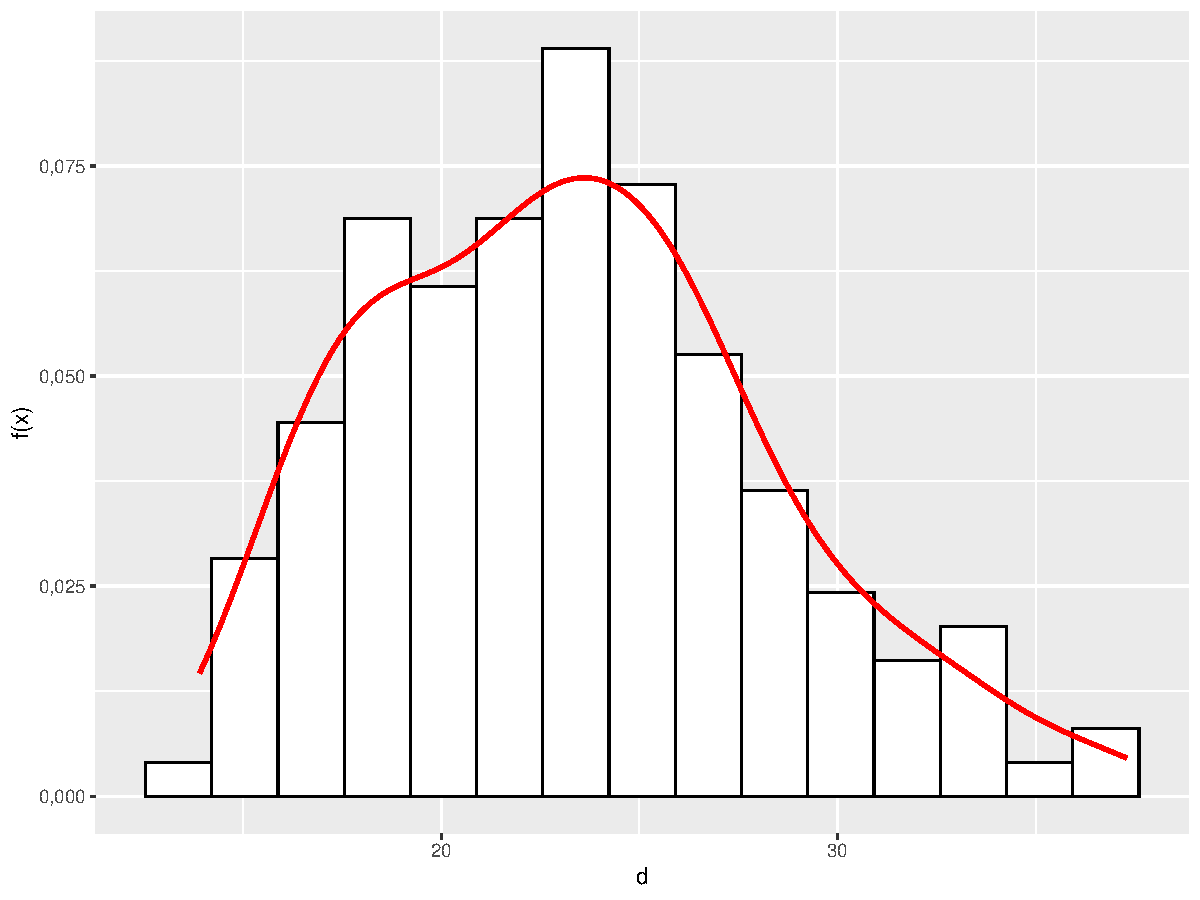
\includegraphics[width=0.8\linewidth]{_main_files/figure-latex/unnamed-chunk-23-1} \caption{Histogramm}\label{fig:unnamed-chunk-23}
\end{figure}

See kood loob R-keeles \texttt{ggplot2} paketiga graafiku, mis visualiseerib andmete jaotust. Vaatame seda samm-sammult:

\begin{enumerate}
\def\labelenumi{\arabic{enumi}.}
\item
  \textbf{\texttt{ggplot(df,\ aes(x))}}: See alustab graafiku loomist. \texttt{df} on andmetabel, mis sisaldab andmeid. \texttt{aes(x)} määrab, et x-teljele kuvatakse muutujat \texttt{x}. See on graafiku ``põhi'', millele järgnevad kihid lisatakse.
\item
  \textbf{\texttt{geom\_histogram(...)}}: See lisab histogrammi.

  \begin{itemize}
  \tightlist
  \item
    \texttt{geom\_histogram()} funktsioon loob histogrammi, mis näitab andmete sagedust erinevatesse gruppidesse jaotatuna.
  \item
    \texttt{aes(y=after\_stat(density))} on oluline osa. See määrab, et y-teljel kuvatakse \emph{tihedust} (density), mitte lihtsalt sagedust (count). \texttt{after\_stat()} funktsiooniga pääsetakse ligi statistilisele väärtusele, mis arvutatakse histogrammi joonistamisel. Tihedus on normaliseeritud sagedus, nii et histogrammi pindala on 1. See võimaldab histogrammi ja tihedusfunktsiooni kõrvuti kuvada.
  \item
    \texttt{fill="white"} määrab histogrammi kastide sisemise värvi valgeks.
  \item
    \texttt{color="black"} määrab histogrammi kastide piirjoone värvi mustaks.
  \end{itemize}
\item
  \textbf{\texttt{geom\_density(color="red",\ lwd=1)}}: See lisab tihedusfunktsiooni graafikule.

  \begin{itemize}
  \tightlist
  \item
    \texttt{geom\_density()} funktsioon arvutab ja joonistab andmete tihedusfunktsiooni, mis on silutud kõver, mis näitab andmete jaotuse kuju.
  \item
    \texttt{color="red"} määrab tihedusfunktsiooni joone värvi punaseks.
  \item
    \texttt{lwd=1} määrab joone paksuse (line width) 1-ks.
  \end{itemize}
\item
  \textbf{\texttt{labs(y\ =\ "f(x)")}}: See lisab y-teljele sildi ``f(x)''. See on hea tava, et telgi selgelt märgistada, eriti kui y-telg näitab tihedust, mitte sagedust. ``f(x)'' on levinud tähistus tõenäosustihedusfunktsioonile (probability density function).
\end{enumerate}

\textbf{Sageduste arvutamine}

Tulpdiagrammile võib eelnevalt välja arvutada antud sagedused. Selleks saab kasutada funktsiooni \texttt{cut()}, mis vajab rühmade piire sisendiks ning seejärel saab juba funktsiooniga \texttt{table()} loendada kokku iga rühma liikmete arvu.

\subsection{Exceli keskkonnas:}\label{exceli-keskkonnas}

\subsubsection{Histogramm}\label{histogramm-1}

Histogrammi loomiseks Excelis peab andmed esmalt sisestama tabelisse ja seejärel kasutama selle jaoks sobivat tööriista.

\begin{enumerate}
\def\labelenumi{\arabic{enumi}.}
\tightlist
\item
  Sisesta pideva tunnuse väärtused Exceli tabelisse.
\item
  Vali need lahtrid, kuhu soovid luua histogrammi.
\item
  Mine menüüsse ``Lisa'' ja vali ``Diagramm''.
\item
  Vali ``Histogramm'' ja klikka ``OK''.
\item
  Seejärel on võimalik vormindada telje suvandeid, millega määratakse rühmade (MS Exceli keskkonnas nimetusega ``salv'') parameetrid.
\end{enumerate}

\subsubsection{Sageduste arvutamine}\label{sageduste-arvutamine}

MS Exceli funktsioon \texttt{FREQUENCY()} võimaldab kasutajatel määrata, kui sageli väärtused esinevad teatud väärtusvahemikes. See funktsioon sobib hästi suurte andmekogumite analüüsimiseks, et mõista andmete jaotust ilma iga üksiku väärtuse manuaalse üle vaatamiseta.

Enne \texttt{FREQUENCY()} funktsiooni kasutamist peate määrama rühmade vahemike piirid, millesse soovite oma andmed jaotada. Need piirid tuleks sisestada eraldi veergu Exceli töölehel. Näiteks, kui soovite analüüsida testitulemusi vahemikus 0-100, võite määrata piirid 0, 20, 40, 60, 80, 100.

\begin{enumerate}
\def\labelenumi{\arabic{enumi}.}
\tightlist
\item
  \textbf{Andmete ja piiride sisestamine:}
\end{enumerate}

\begin{itemize}
\tightlist
\item
  Sisestage oma andmekogum ühte veergu (nt A2:A101).
\item
  Sisestage vahemike piirid teise veergu (nt B2:B7, eeldades, et esitasite näiteks eelmises punktis toodud piirid).
\end{itemize}

\begin{enumerate}
\def\labelenumi{\arabic{enumi}.}
\setcounter{enumi}{1}
\tightlist
\item
  \textbf{Funktsiooni rakendamine:}
\end{enumerate}

\begin{itemize}
\tightlist
\item
  Valige tühi ala, kuhu soovite tulemused väljastada. Sellel peaks olema sama palju lahtrid kui määratletud vahemike piire. Kui teil on 6 piiri, valige 6 lahtrit vertikaalselt.
\item
  Sisestage \texttt{FREQUENCY()} funktsioon. Kuna \texttt{FREQUENCY()} on massiivifunktsioon, tuleb see sisestada massiivivalemiga. Algusesse minev andmevahemik on teie andmekogum ja teine vahemik on teie vahemike piirid.
  Näiteks: \texttt{=FREQUENCY(A2:A101,\ B2:B7)}
\item
  Pärast funktsiooni sisestamist lõpetage sisestus, vajutades \textbf{Ctrl+Shift+Enter}. Excel käitab nüüd \texttt{FREQUENCY()} funktsiooni massiivina ja täidab valitud lahtrid andmete sagedustega, mis vastavad määratud vahemikele.
\end{itemize}

\chapter{Karakteristikud}\label{karakteristikud}

Statistilised karakteristikud on kvantitatiivsed või kvalitatiivsed omadused, mis kirjeldavad ja iseloomustavad andmekogumeid või andmete jaotusi. Neid kasutatakse andmete kokkuvõtlikuks esitamiseks, et saada aru andmete üldisest käitumisest, trendidest ja omadustest. Statistilised karakteristikud võimaldavad teha järeldusi kogu populatsiooni kohta, analüüsides selleks valimit. Peamised statistilised karakteristikud jagunevad kaheks suureks rühmaks: keskmise ja hajuvuse karakteristikud.

Juhuslik suurus on täielikult kirjeldatud üldkogumi jaotus- või tihedusfunktsiooniga (jaotusega). Juhusliku suuruse iseloomustamiseks teatud aspektist kasutatakse erinevaid arvkarakteristikuid. Neist tähtsaim on \textbf{keskväärtus} ehk matemaatiline ootus, mida tähistatakse EX ja mis on defineeritud järgnevalt.

Pideva juhusliku suuruse korral:
\[EX = \sum_{-\infty}^{\infty} x \cdot f(x) dx\]

Diskreetse juhusliku suuruse korral:
\[EX = \sum_{i=1}^{n} x_i \cdot p_i\]

\section{Keskmised}\label{keskmised}

\subsection{Aritmeetiline keskmine}\label{aritmeetiline-keskmine}

Juhusliku suuruse jaotusseadus on uurijale enamasti teadmata. Seetõttu kasutatakse üldkogumi karakteristikute hindamiseks valimi vastavaid karakteristikuid. Üldkogumi keskväärtusele vastab valimi aritmeetiline keskmine, mida tähistatakse ülakriipsuga vastava muutuja kohal \(\bar x\) ja arvutatakse järgnevalt.

\[ \bar x=\frac{1}{N}\sum_{i=1}^{k}n_i \cdot x_i \]

Kus \(x_{i}\) on iga andmehulga liige ning \(n\) on andmehulga suurus.

\textbf{R keskkonnas:}

\begin{Shaded}
\begin{Highlighting}[]
\CommentTok{\# Laadime proovitükkide andmed}
\NormalTok{df }\OtherTok{\textless{}{-}}\NormalTok{ readxl}\SpecialCharTok{::}\FunctionTok{read\_excel}\NormalTok{(}\StringTok{"data/naited.xlsx"}\NormalTok{,}\StringTok{"prt\_andmed"}\NormalTok{)}
\CommentTok{\# Tunnusest arvutatakse keskmine:}
\FunctionTok{mean}\NormalTok{(df}\SpecialCharTok{$}\NormalTok{d)}
\end{Highlighting}
\end{Shaded}

\begin{verbatim}
[1] 23,3
\end{verbatim}

\textbf{Exceli keskkonnas:}

\begin{Shaded}
\begin{Highlighting}[]
\NormalTok{=MEAN(andme\_vektor)}
\end{Highlighting}
\end{Shaded}

\subsection{Ruutkeskmine}\label{ruutkeskmine}

Ruutkeskmine on üks keskmise leidmise meetoditest, mis annab ülevaate andmehulgast ning aitab mõõta andmete hajuvust. Ruutkeskmise leidmiseks tuleb iga andmehulga liige ruutu võtta, seejärel leida nende aritmeetiline keskmine ning võtta sellest ruutjuur. Matemaatiliselt väljendatuna on ruutkeskmine järgmine:

\[ \bar x_{ruut}=\sqrt{\frac{1}{N}\sum_{i=1}^{k}n_i \cdot x_i^2} \],

kus \(x_{i}\) on iga andmehulga liige ning \(n\) on andmehulga suurus.

Metsanduses on ruutkeskmine kasutusel keskmise diameetri arvutamisel.

\textbf{R keskkonnas:}

\begin{Shaded}
\begin{Highlighting}[]
\CommentTok{\# Tunnusest arvutatakse ruut ning keskmisest võetakse ruutjuur:}
\FunctionTok{sqrt}\NormalTok{(}\FunctionTok{mean}\NormalTok{(df}\SpecialCharTok{$}\NormalTok{d}\SpecialCharTok{\^{}}\DecValTok{2}\NormalTok{))}
\end{Highlighting}
\end{Shaded}

\begin{verbatim}
[1] 23,8
\end{verbatim}

\textbf{Exceli keskkonnas:}

\begin{Shaded}
\begin{Highlighting}[]
\NormalTok{=SQRT(MEAN(andmeplokk\^{}2))}
\end{Highlighting}
\end{Shaded}

\subsection{Geomeetriline keskmine}\label{geomeetriline-keskmine}

Geomeetriline keskmine on keskmise arvutamise meetod, mille puhul kõik antud arvud korrutatakse omavahel ning seejärel võetakse saadud korrutisest n-nda astme juur, kus n tähistab arvude kogust. Geomeetriline keskmine \(\bar x_{geom}\) arvutatakse järgneva valemiga:

\[\bar x_{geom}=\exp \biggl( \frac{1}{N}\sum_{i=n}^k n_i \cdot \ln(x_i) \biggr) \]

kus:

\begin{itemize}
\tightlist
\item
  \(n\) on arvude kogus
\item
  \(x_1, x_2, \ldots, x_n\) on positiivsed arvud
\end{itemize}

\textbf{R keskkonnas:}

\begin{Shaded}
\begin{Highlighting}[]
\CommentTok{\# Tunnusest arvutatakse logaritm ning keskmisest võetakse exponent:}
\FunctionTok{exp}\NormalTok{(}\FunctionTok{mean}\NormalTok{(}\FunctionTok{log}\NormalTok{(df}\SpecialCharTok{$}\NormalTok{d)))}
\end{Highlighting}
\end{Shaded}

\begin{verbatim}
[1] 22,7
\end{verbatim}

\textbf{Exceli keskkonnas:}

\begin{Shaded}
\begin{Highlighting}[]
\NormalTok{=GEOMEAN(andmeplokk)}
\end{Highlighting}
\end{Shaded}

\subsection{Harmooniline keskmine}\label{harmooniline-keskmine}

Harmooniline keskmine on statistiline mõõde, mis arvutatakse jagades arvude hulk nende vastandväärtuste summa järgi. Harmooniline keskmine on erinev aritmeetilisest ja geomeetrilisest keskmisest ning seda kasutatakse eelkõige siis, kui on vaja leida keskmine, mis arvestab vastandväärtusi või suhtarve.

Harmoonilist keskmist kasutatakse sageli olukordades, kus on vaja arvutada keskmine mingis suhtarvulises kontekstis, näiteks kiiruste, ajade või muude vastandväärtustega seotud suuruste puhul. Näiteks võib harmooniline keskmine kiirus olla kasulik, kui on vaja arvutada keskmine kiirus teepikkuse ja sõiduaegadega seotud olukorras.

Harmoonilist keskmist arvutatakse valemiga:
\[\bar x_{harm} = \frac{N}{\sum_{i=1}^k n_i / x_i},\]
kus \(x_{1}, x_{2}, \ldots, x_{n}\) on arvude hulk, mille harmoonilist keskmist soovitakse leida ning \(n\) on arvude hulga suurus.

\textbf{R keskkonnas:}

\begin{Shaded}
\begin{Highlighting}[]
\CommentTok{\# Tunnuse pöördväärtuse keskmisest võetakse pöördväärtus:}
\DecValTok{1}\SpecialCharTok{/}\FunctionTok{mean}\NormalTok{(}\DecValTok{1}\SpecialCharTok{/}\NormalTok{df}\SpecialCharTok{$}\NormalTok{d)}
\end{Highlighting}
\end{Shaded}

\begin{verbatim}
[1] 22,2
\end{verbatim}

\textbf{Exceli keskkonnas:}

\begin{Shaded}
\begin{Highlighting}[]
\NormalTok{=HARMEAN(andmeplokk)}
\end{Highlighting}
\end{Shaded}

\section{Kvantiilid}\label{kvantiilid}

Juhusliku suuruse p-kvantiiliks (0 \textless{} p \textless{} 1) nimetatakse sellist juhusliku suuruse väärtust xp, millest väiksemate väärtuste esinemise tõenäosus on p:

\[ P (X < x_p) = p \]

Teatud kvantiilide jaoks kasutatakse erinimetusi:

\begin{itemize}
\tightlist
\item
  \(x_{0,50}\) -- mediaan, tähistatakse ka Me;
\item
  \(x_{0,25}\) -- alumine kvartiil;
\item
  \(x_{0,75}\) -- ülemine kvartiil;
\item
  \(x_{0,10}\) -- alumine detsiil;
\item
  \(x_{0,9}\) -- ülemine detsiil;
\item
  \(x_{0,01}\) -- alumine protsentiil;
\item
  \(x_{0,99}\) -- ülemine protsentiil.
\end{itemize}

Enamkasutatavam kvantiil on \textbf{mediaan}, mida võib pidada (nagu keskväärtustki) juhusliku suuruse tsentriks. Mediaan on juhusliku suuruse selline väärtus, millest nii väiksemate kui ka suuremate väärtuste esinemise tõenäosus on 0,5. Mediaan iseloomustab juhusliku suuruse asendi poolest keskmist väärtust.
Kui on teada juhusliku suuruse jaotusfunktsioon F(x), siis saab juhusliku suuruse kvantiili xp arvutada kui jaotusfunktsiooni pöördfunktsiooni, sest kvantiili definitsioonist tuleneb F(xp) = p.~Juhul kui on tegemist vaatlusandmestikuga, saab kvantiile ligikaudu hinnata empiiriliselt jaotusfunktsiooni graafikult.

\section{Mediaan}\label{mediaan}

Mediaan väärtus, mis jagab andmed kaheks võrdselt suureks pooleks. See ei sõltu ekstreemsetest väärtustest ega hajutatud andmetest.

Mediaani arvutamine:

\begin{Shaded}
\begin{Highlighting}[]
\FunctionTok{median}\NormalTok{(df}\SpecialCharTok{$}\NormalTok{d)}
\end{Highlighting}
\end{Shaded}

\begin{verbatim}
[1] 23,2
\end{verbatim}

Exceli keskkonnas:

\begin{Shaded}
\begin{Highlighting}[]
\NormalTok{=MEDIAN(andmeplokk)}
\end{Highlighting}
\end{Shaded}

\chapter{Jaotusfunktsioonid}\label{jaotusfunktsioonid}

Statistikas nimetatakse \textbf{jaotusfunktsiooniks} funktsiooni, mis kirjeldab juhusliku suuruse \(X\) tõenäosusjaotust. See määrab iga reaalarvu \(x\) korral tõenäosuse, et juhusliku suuruse \(X\) väärtus on väiksem või võrdne \(x\)-ga. Formaalselt väljendub jaotusfunktsioon kui \(F(x) = P(X \leq x)\), seostes iga \(x\)-i väärtuse vastavusse tõenäosuse \(P(X \leq x)\).

Jaotusfunktsiooni saab kasutada nii pidevate kui ka diskreetsete juhuslike suuruste puhul. Pideva juhusliku suuruse korral on jaotusfunktsioon integraal tema tihedusfunktsioonist. Diskreetse juhusliku suuruse korral on jaotusfunktsioon kumulatiivne tõenäosuste summa.

Jaotusfunktsioonil on järgmised omadused:

\begin{itemize}
\tightlist
\item
  See on \emph{monotoonselt kasvav}, st \(F(x) \le F(y)\) kui \(x \le y\).
\item
  See on \emph{paremalt pidev}, st \(\lim_{x \to y^+} F(x) = F(y)\) iga \(y\) korral.
\item
  See läheneb 0-le kui \(x\) läheneb \(-\infty\)-le, ja 1-le kui \(x\) läheneb \(+\infty\)-le.
\end{itemize}

Jaotusfunktsiooni saab kasutada juhusliku suuruse tõenäosusjaotuse visualiseerimiseks. Selle abil saab arvutada ka tõenäosusi, et juhuslik suurus langeb teatud vahemikku. Näiteks tõenäosus, et X langeb vahemikku {[}a, b{]}, on F(b) - F(a).

Jaotusfunktsioon on statistikas väga oluline tööriist. See aitab mõista juhuslike suuruste käitumist ja teha järeldusi andmete kohta.

Lisaks ülaltoodule on jaotusfunktsioonil veel teisi olulisi omadusi ja kasutusvõimalusi. Näiteks:

\begin{itemize}
\tightlist
\item
  Jaotusfunktsiooni abil saab leida juhusliku suuruse kvantiile. Kvantiil on väärtus, millest väiksemaks või võrdseks jääb juhusliku suuruse väärtus teatud tõenäosusega.
\item
  Jaotusfunktsiooni abil saab arvutada juhusliku suuruse keskväärtust, dispersiooni ja teisi momente.
\item
  Jaotusfunktsiooni abil saab genereerida juhuslikke arve, mis järgivad teatud jaotust.
\end{itemize}

Jaotusfunktsioon on statistikas fundamentaalne mõiste ja sellel on lai valik rakendusi.

Teoreetilisi jaotusi kasutatakse hüpoteeside testimisel statistilistes analüüsides selleks, et teha kindlaks, kas vaatlusandmete hajuvus on juhuslik või on olemas mingi muster või seos. Oluline on märkida, et enamik statistilisi teste eeldab teatud jaotuse tundmist, mille põhjal tehakse järeldusi populatsiooni kohta.

Kõige tuntum teoreetiline jaotus on normaaljaotus, mis on sümmeetriline kõver ning annab tihti paljudele looduslikele nähtustele lähedase jaotuse. Normaaljaotus on oluline paljudes statistilistes testimistes, näiteks t-testis või ANOVA analüüsis. Kui andmed järgivad normaaljaotust, saab kasutada erinevaid statistilisi meetodeid.

Lisaks normaaljaotusele on olulised ka teised jaotused, nagu näiteks binoomjaotus (kasutatakse binomiaalsete katsete puhul), eksponentsiaaljaotus (kasutatakse elupikkuste analüüsimisel) ja Poissoni jaotus (kasutatakse haruldaste sündmuste analüüsimisel).

Hüpoteeside testimisel võrreldakse empiirilisi andmeid teoreetiliste jaotustega, et teha järeldusi populatsiooni kohta. Näiteks võib uurida, kas kahe rühma keskmiste vahel on oluline erinevus või kas mingi seos on juhuslik või mitte. Sellisel juhul kasutatakse statistilisi teste, et hinnata, kas tulemus võib olla juhuslik või on tõenäoliselt tingitud tegelikust mõjust või seosest.

\section{Hüpotees}\label{huxfcpotees}

Hüpotees on statistikas väide või eeldus, millele toetudes teostatakse uuringuid, analüüsi või katseid. Hüpotees võib olla kas uurija poolt esitatud eeldus, mida on vaja tõestada või ümber lükata või juba olemasolev teooria, mida soovitakse kontrollida.

\begin{itemize}
\item
  \textbf{Nullhüpotees (H0)}: See on väide, mida püütakse ümber lükata. Nullhüpotees eeldab, et uuritavas populatsioonis puudub mingi mõju, seos või erinevus. Näiteks võib nullhüpotees väita, et kahe rühma keskmised väärtused on võrdsed või et tunnus ei mõjuta teise tunnuse jaotust. Nullhüpotees on alati konkreetne väide, mille kohta on võimalik arvutada tõenäosust.
\item
  \textbf{Sisukas ehk alternatiivne hüpotees (H1)}: See on väide, mida uurija soovib tõestada. See hüpotees esitab oletuse mingi mõju, seose või erinevuse olemasolu kohta populatsioonis. Näiteks võib alternatiivne hüpotees väita, et kahe rühma keskmised väärtused on erinevad või et tunnus mõjutab teise tunnuse jaotust. Sisukaid hüpoteese võib olla ka rohkem kui üks.
\item
  Hüpoteesipaar püstitatakse üldkogumi jaoks.
\item
  Hüpoteeside püstitus sõltub uurimisküsimusest ja sellest, kas oodatakse kindlasuunalist kõrvalekallet või mitte.

  \begin{itemize}
  \tightlist
  \item
    \textbf{Kahepoolne hüpotees:} Kontrollitakse, kas parameeter (nt keskväärtus) erineb mingist väärtusest. Näiteks H0: \(\mu\) = \(\mu_0\) ja H1: \(\mu\) \(\neq\) \(\mu_0\).
  \item
    \textbf{Ühepoolne hüpotees:} Kontrollitakse, kas parameeter on suurem või väiksem mingist väärtusest. Näiteks H0: \(\mu\) \(\le\) \(\mu_0\) ja H1: \(\mu\) \textgreater{} \(\mu_0\) (parempoolne) või H0: \(\mu\) \(\ge\) \(\mu_0\) ja H1: \(\mu\) \textless{} \(\mu_0\) (vasakpoolne).
  \end{itemize}
\item
  \textbf{Olulisuse nivoo (\(\alpha\))}: See on tõenäosus, millega ollakse nõus tegema I liiki viga ehk lükkama tagasi kehtiva nullhüpoteesi. Tavaliselt kasutatakse olulisuse nivood 0,05 (5\%) või 0,01 (1\%), kuid see sõltub uurimisvaldkonnast. Mida väiksem on olulisuse nivoo, seda väiksem on tõenäosus teha I liiki viga. Olulisuse nivoo on maksimaalne lubatud p-väärtus väärtus.
\item
  \textbf{Kriitilised väärtused:} Need on teststatistiku väärtused, mis määratlevad kriitilise piirkonna. Kriitilised väärtused leitakse teststatistiku jaotusest vastavalt valitud olulisuse nivool.

  \begin{itemize}
  \tightlist
  \item
    Kahepoolse hüpoteesi korral on kaks kriitilist väärtust, mis asuvad jaotuse mõlemal pool.
  \item
    Ühepoolse hüpoteesi korral on üks kriitiline väärtus, mis asub kas jaotuse paremal või vasakul pool.
  \item
    Kriitilised väärtused on seotud ka usaldusvahemiku laiusega.
  \end{itemize}
\item
  \textbf{Teststatistiku väärtuse võrdlemine kriitilise väärtusega:} Võrreldakse, kas empiiriline teststatistiku väärtus langeb kriitilisse piirkonda.

  \begin{itemize}
  \tightlist
  \item
    Kui empiiriline väärtus ületab kriitilise väärtuse (langeb kriitilisse piirkonda), siis lükatakse nullhüpotees tagasi ja võetakse vastu sisukas hüpotees.
  \item
    Kui empiiriline väärtus ei lange kriitilisse piirkonda, siis ei ole alust nullhüpoteesi tagasi lükata. Jäädakse nullhüpoteesi juurde, aga see ei tähenda, et nullhüpotees on tõestatud.
  \end{itemize}
\item
  \textbf{Olulisuse tõenäosus (p-väärtus):} See on tõenäosus saada antud või veelgi äärmuslikum valim, eeldusel, et nullhüpotees on tõene. Mida väiksem on p-väärtus, seda väiksem on tõenäosus, et nullhüpotees kehtib.

  \begin{itemize}
  \tightlist
  \item
    Kui p-väärtus on väiksem kui olulisuse nivoo (p \textless{} \(\alpha\)), siis lükatakse nullhüpotees tagasi.
  \item
    Kui p-väärtus on suurem või võrdne olulisuse nivooga (p \(\ge\) \(\alpha\)), siis ei lükata nullhüpoteesi tagasi.
  \item
    Olulisuse tõenäosust saab kasutada nullhüpoteesi sobivuse hindamiseks antud valimiga.
  \end{itemize}
\item
  Teststatistiku empiirilise väärtuse võrdlemine kriitilise väärtusega ja olulisuse tõenäosuse võrdlemine olulisuse nivooga on ekvivalentsed meetodid.
\end{itemize}

Tuleb arvestada, et nullhüpoteesi ei saa ``tõestada'', kuna statistiliste testidega ei saa nullhüpoteesi tõestada samamoodi, nagu matemaatikas võidakse tõestada väiteid. Selle asemel saab statistiliste testide abil hinnata, kas on piisavalt tõendeid nullhüpoteesi tagasilükkamiseks. Kui testi tulemus näitab, et andmed on nullhüpoteesiga vastuolus, siis võidakse nullhüpotees tagasi lükata. Kui aga testi tulemus ei näita olulist vastuolu nullhüpoteesiga, siis ei lükata nullhüpoteesi tagasi. Siiski, see ei tähenda, et nullhüpotees oleks ``tõestatud''; pigem öeldakse, et ei leitud piisavalt tõendeid nullhüpoteesi ümberlükkamiseks. Oluline on mõista, et nullhüpoteesi mitte-tagasilükkamine ei tõesta selle paikapidavust. See viitab lihtsalt sellele, et andmed ei andnud piisavalt alust nullhüpoteesi ümber lükata. Samuti on oluline meeles pidada, et statistiliste testide tulemused annavad ainult tõenäosusliku hinnangu ning need tuleb alati panna laiemasse konteksti koos teiste tõendite ja teadmistega valdkonnast.

\section{Jaotusfunktsioon}\label{jaotusfunktsioon}

Jaotusfunktsioon on viis näidata, kui tõenäoline on, et mingi arv (mida me nimetame muutujaks) on väiksem või võrdne kindla arvuga x. See aitab meil mõista, kuidas arvud (või muutujad) ühes grupis paiknevad või jaotuvad, näiteks kui me tahame teada, kui tõenäoline on, et metsa pindala on teatud suurusega või väiksem.

Jaotusfunktsiooni olulised omadused on:

\begin{enumerate}
\def\labelenumi{\arabic{enumi}.}
\item
  Vahemik: jaotusfunktsioon võtab väärtuseid 0 ja 1 vahemikus, mis tähendab, et tõenäosus on alati selles vahemikus.
\item
  Mittelangus: jaotusfunktsioon ei kasva kunagi tagurpidi; see liigub alati kas võrdse kõrguse juurde või kõrgemale.
\item
  Ühekordsus: Ükskõik millised on väärtused, jaotusfunktsiooni koguulatus on alati 1.
\end{enumerate}

Jaotusfunktsiooni abil saame lahendada paljusid statistilisi ülesandeid. See aitab meil leida näiteks keskmisi väärtusi, hajuvust (ehk kui laiali arvud on jaotunud), tõenäosusi (kui tõenäoline on mingi sündmus), ja isegi määrata arvude jaotuse erinevaid tasemeid. See tähendab, et jaotusfunktsioon on tööriist, mis aitab meil mõista, kuidas andmed käituvad, ja teha selle põhjal täpseid otsuseid või järeldusi.

\begin{Shaded}
\begin{Highlighting}[]
\CommentTok{\# Näide R keskkonnas}
\CommentTok{\# Laadime peatükis kasutatavad paketid}
\FunctionTok{library}\NormalTok{(dplyr)}
\FunctionTok{library}\NormalTok{(ggplot2)}
\FunctionTok{library}\NormalTok{(ggpmisc)}
\end{Highlighting}
\end{Shaded}

\begin{itemize}
\tightlist
\item
  \textbf{Andmete jaotus.} ECDF graafik annab intuitiivse ülevaate andmete jaotusest, näidates, kui suur osa andmestikust on alla või võrdne iga võimaliku väärtusega. See on eriti kasulik andmete jaotuse mõistmiseks ilma eeldamata mingit konkreetset jaotustüüpi.
\end{itemize}

ECDF graafik on väärtuslik tööriist andmete uurimisel, võimaldades kiiresti hinnata andmete jaotuse omadusi ja tuvastada andmete levikuga seotud probleeme.

\begin{Shaded}
\begin{Highlighting}[]
\CommentTok{\# Laadime proovitükkide andmed}
\NormalTok{df }\OtherTok{\textless{}{-}}\NormalTok{ readxl}\SpecialCharTok{::}\FunctionTok{read\_excel}\NormalTok{(}\StringTok{"data/naited.xlsx"}\NormalTok{,}\StringTok{"prt\_andmed"}\NormalTok{)}

\FunctionTok{ggplot}\NormalTok{(df, }\FunctionTok{aes}\NormalTok{(d)) }\SpecialCharTok{+}
  \FunctionTok{stat\_ecdf}\NormalTok{()}
\end{Highlighting}
\end{Shaded}

\begin{figure}
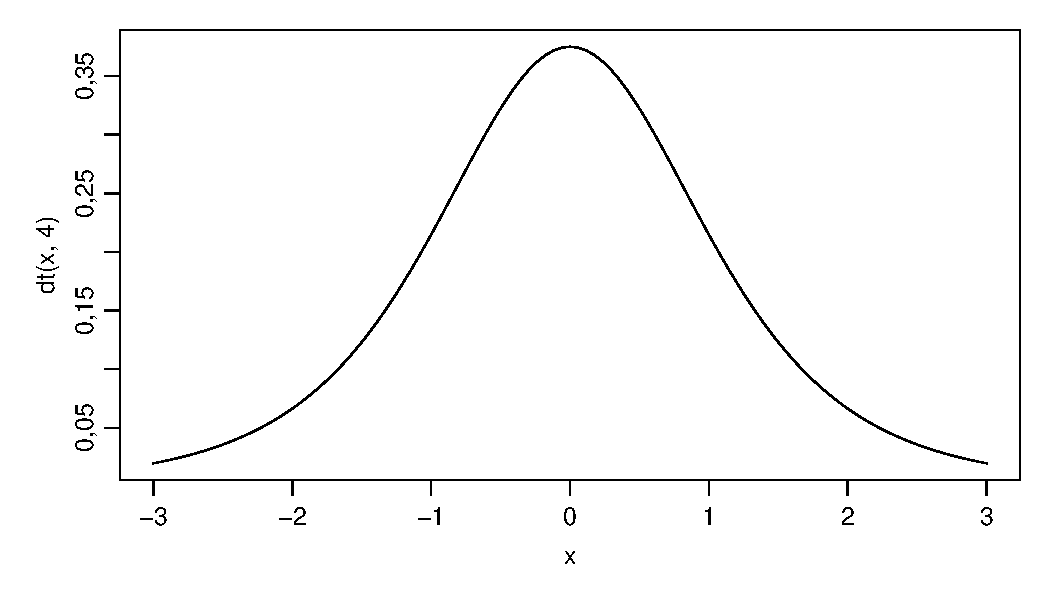
\includegraphics[width=0.8\linewidth]{_main_files/figure-latex/unnamed-chunk-38-1} \caption{Empiiriline jaotusfunktsioon.}\label{fig:unnamed-chunk-38}
\end{figure}

Selgitus:

\begin{itemize}
\item
  \textbf{\texttt{ggplot(df,\ aes(d))}}: See algatab graafiku loomise, kasutades \texttt{ggplot2}.

  \begin{itemize}
  \tightlist
  \item
    \texttt{ggplot(df,\ ...)} määrab, et graafiku andmed pärinevad \texttt{df} andmeraamist.
  \item
    \texttt{aes(x)} seostab andmeraami veeru \texttt{d} graafiku x-teljega. See ütleb ggplot2-le, et veeru \texttt{x} väärtused määravad punktide asukoha horisontaalteljel.
  \end{itemize}
\item
  \textbf{\texttt{+\ stat\_ecdf()}}: See lisab graafikule kihi, nimelt ECDF-i.

  \begin{itemize}
  \tightlist
  \item
    \texttt{stat\_ecdf()} arvutab ECDF-i. ECDF antud väärtusel \emph{x} tähistab andmepunktide osakaalu, mis on väiksemad või võrdsed \emph{x}-ga.
  \end{itemize}
\end{itemize}

\section{Tihedusfunktsioon}\label{tihedusfunktsioon}

Tihedusfunktsioon on statistikas kasutatav funktsioon, mis kirjeldab tõenäosust, et juhuslik suurus langeb mingisse kindlasse vahemikku. Tihedusfunktsiooni saab kasutada tõenäosusjaotuse (nt normaaljaotus, Bernoulli jaotus jne) karakteriseerimiseks. See näitab, kui tõenäoline on konkreetse väärtuse saamine selle jaotuse järgi.

Tihedusfunktsioon on graphiline joon, mis esitab tõenäosuse jaotuse ühtlase tervikuna. Üksiku väärtuse tõenäosus on antud tihedusfunktsiooni abil vahemikuna, mida funktsioon katab selles punktis. Tavaliselt on tihedusfunktsioon positiivne ja integreerub üle vahemiku 1, mis tähendab, et kõikidele võimalikele väärtustele vastavate tõenäosuste summa on alati 1.

Metsanduses võib tihedusfunktsiooni kasutada näiteks puistu tiheduse jaotuse kirjeldamisel, kus tihedusfunktsioon näitab puude arvu tõenäosust kindlas pindalas. Tihedusfunktsioonide abil saab hinnata erinevaid statistilisi parameetreid nagu keskmine, mediaan, variatsioon jt, ning teha ennustusi ja otsuseid metsaressursi haldamisel ja planeerimisel.

Tihedusfunktsioon (inglise keeles probability density function, lühidalt PDF) on statistikas oluline mõiste, mida kasutatakse tõenäosusjaotuse kirjeldamiseks. Tihedusfunktsioon annab meile informatsiooni selle kohta, kuidas on tõenäosus mingi juhusliku muutuja väärtuse jaotustel. Allpool on toodud mõned olulised statistilised omadused tihedusfunktsiooni kohta:

Integreeruvus: tihedusfunktsioon peab olema integreeruv kogu kandva ala suhtes, st selle integraal alates miinimum- kuni maksimumväärtuseni peab olema võrdne ühega. Teisisõnu, kogu võimaliku vaadeldava mahu (nt kogu metsaala, kus uuritakse puude tihedust) peab olema 100\%.

Positiivsus: Tihedusfunktsiooni väärtused peavad olema alati positiivsed. See tähendab, et tõenäosus väärtuse sattumiseks konkreetsesse intervalli ei saa olla negatiivne.

Normaliseerumine: Tihedusfunktsioon peab olema normaliseeritud, mis tähendab, et alati, kui me integreerime tihedusfunktsiooni kogu liinil või tasandil, siis tulemuseks peab olema üks. See tagab, et tihedusfunktsioon annab meile täpse tõenäosuse, et vaadeldav suurus langeb mingisse kindlasse vahemikku.

Mitte-negatiivsus: Tihedusfunktsioon ei või mitte kunagi võtta negatiivseid väärtusi. See tähendab, et tõenäosus mingi suuruse väärtuse jaoks on alati null või suurem.

Tipukoha lokaliseerimine: Tihedusfunktsiooni tippkoht näitab moodi ehk suurimat tõenäosust mingi väärtuse saamiseks. Mood on statistikas näitaja, mis näitab, milline väärtus esineb andmehulgas kõige sagedamini ehk mis väärtusega esineb andmehulkade hulgas enim kordi. Mood on üks keskmiste näitajate tüüpe, mis aitab anda ülevaadet andmete esinemissagedusest konkreetse väärtuse juures.

Need omadused on olulised tihedusfunktsiooni mõistmisel ja kasutamisel statistilistes analüüsides, sealhulgas metsanduses, kus tihedusfunktsiooni abil saab kirjeldada erinevaid muutujaid nagu puu tihedus, metsa elujõulisus jne.

Näide R-i koodist, mis genereerib normaaljaotuse tihedusfunktsiooni graafiku:

\begin{Shaded}
\begin{Highlighting}[]
\CommentTok{\# Loome andmestiku}
\FunctionTok{ggplot}\NormalTok{(df, }\FunctionTok{aes}\NormalTok{(d)) }\SpecialCharTok{+}
  \FunctionTok{geom\_density}\NormalTok{()}
\end{Highlighting}
\end{Shaded}

\begin{figure}
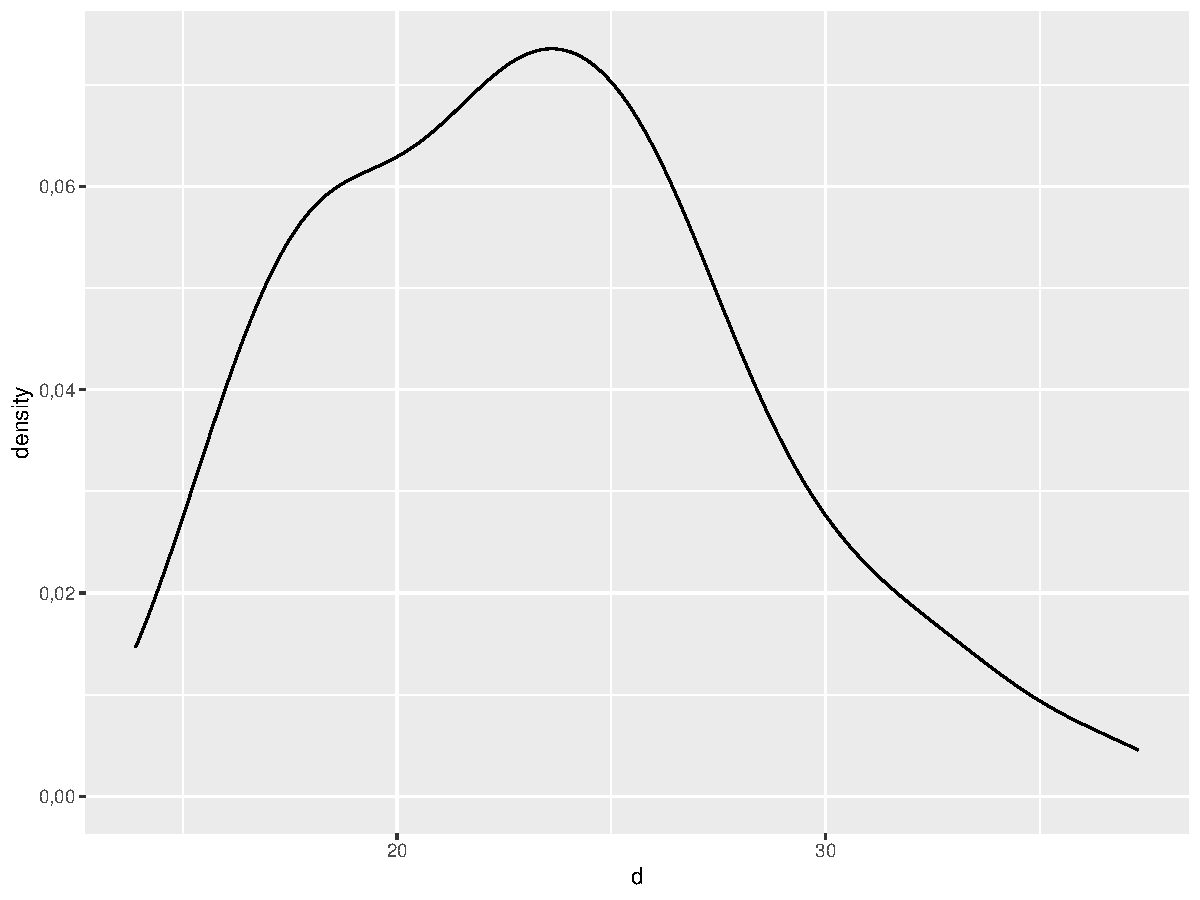
\includegraphics[width=0.8\linewidth]{_main_files/figure-latex/unnamed-chunk-39-1} \caption{Empiiriline tihedusfunktsioon.}\label{fig:unnamed-chunk-39}
\end{figure}

See kood genereerib normaaljaotuse tihedusfunktsiooni graafiku, kus x-teljel on andmete väärtused ja y-teljel tihedusfunktsiooni väärtused.

\section{Normaaljaotus}\label{normaaljaotus}

Normaaljaotus on statistikas ja tõenäosusteoorias üks tähtsamaid pidevaid jaotusi. Selle tunnusmärk on kellakujuline sümmeetriline graafik, mistõttu seda nimetatakse sageli ka Gaussi jaotuseks, kuna seda uuris põhjalikult Carl Friedrich Gauss. Normaaljaotuse keskmes paikneb enamik väärtusi, harvemini esinevad väärtused jäävad aga sellest kaugemale.

\textbf{Normaaljaotuse omadused}

\begin{itemize}
\tightlist
\item
  \textbf{Sümmeetria:} Normaaljaotus on sümmeetriline keskväärtuse suhtes, mis tähendab, et jaotuse graafiku mõlemad pooled on üksteise peegelpildid.
\item
  \textbf{Keskmine, mediaan ja mood:} Normaaljaotuse korral on aritmeetiline keskmine, mediaan ja mood võrdsed.
\item
  \textbf{Hajuvus:} Normaaljaotust iseloomustab hajuvus, mida mõõdetakse standardhälbe abil. Standardhälve näitab, kui palju väärtused keskmisest erinevad.
\item
  \textbf{Ekstsess (kurtosis):} Normaaljaotuse püstakus on null. Püstakus näitab, kui terav on jaotuse tipp.
\item
  \textbf{Asümmeetria (skewness):} Normaaljaotus on asümmeetriline, mis tähendab, et jaotus ei kaldu ei vasakule ega paremale.
\item
  \textbf{Väärtuste jaotus:} Normaaljaotuse puhul jääb umbes 68,3\% väärtustest ühe standardhälbe kaugusele keskmisest, umbes 95,4\% väärtustest kahe standardhälbe kaugusele keskmisest ja umbes 99,7\% väärtustest kolme standardhälbe kaugusele keskmisest.
\item
  \textbf{Teoreetiline ulatus:} Teoreetiliselt võib normaaljaotusega muutuja omada väärtusi vahemikus \(-$inf$\) kuni \($inf$\).
\end{itemize}

\textbf{Normaaljaotuse kasutusalad}

Normaaljaotust kasutatakse laialdaselt statistikas ja erinevates teadusvaldkondades.

\begin{itemize}
\tightlist
\item
  \textbf{Andmete kirjeldamine ja analüüs:}

  \begin{itemize}
  \tightlist
  \item
    Normaaljaotust kasutatakse üldkogumi keskväärtuse usaldusvahemike arvutamiseks.
  \item
    Normaaljaotust kasutatakse sageli hüpoteeside testimisel.
  \item
    Normaaljaotust kasutatakse andmete standardiseerimiseks.
  \item
    Normaaljaotust saab kasutada erindite tuvastamiseks.
  \end{itemize}
\item
  \textbf{Tsentraalne piirteoreem:}

  \begin{itemize}
  \tightlist
  \item
    Tsentraalse piirteoreemi kohaselt alluvad piisavalt suure valimi keskmised ligikaudu normaaljaotusele.
  \end{itemize}
\item
  \textbf{Statistilised mudelid:}

  \begin{itemize}
  \tightlist
  \item
    Normaaljaotust kasutatakse regressioonimudelite vigade jaotuse eelduseks.
  \end{itemize}
\item
  \textbf{Tõenäosusteooria:}

  \begin{itemize}
  \tightlist
  \item
    Normaaljaotust kasutatakse tõenäosusteooria arvutustes.
  \end{itemize}
\item
  \textbf{Rakendusalad:}

  \begin{itemize}
  \tightlist
  \item
    Normaaljaotust kasutatakse paljudes valdkondades, nagu majandus, meditsiin, inseneriteadused, psühholoogia ja keskkonnateadused.
  \end{itemize}
\end{itemize}

\textbf{Standardiseeritud normaaljaotus}

Standardiseeritud normaaljaotus on normaaljaotuse erijuhtum, mille keskmine on 0 ja standardhälve on 1.

\textbf{Normaaljaotuse piirangud}

\begin{itemize}
\tightlist
\item
  Normaaljaotus eeldab andmete sümmeetriat ja teatud hajuvust.
\item
  Normaaljaotus ei ole sobiv ekstremaalsete väärtuste analüüsimiseks.
\item
  Normaaljaotuse omadused kehtivad suure valimi korral.
\end{itemize}

R-is on järgnevad normaaljaotuse funktsioonid:

\begin{itemize}
\tightlist
\item
  \texttt{pnorm()} arvutab tõenäosuse, et juhuslik muutuja on väiksem või võrdne kui antud väärtus.
\item
  \texttt{dnorm()} arvutab tõenäosustihedusfunktsiooni väärtuse antud punktis.
\item
  \texttt{qnorm()} arvutab väärtuse, millest väiksem või võrdne on antud protsent andmetest.
\end{itemize}

\begin{Shaded}
\begin{Highlighting}[]
\FunctionTok{pnorm}\NormalTok{(}\FloatTok{1.96}\NormalTok{, }\DecValTok{0}\NormalTok{, }\DecValTok{1}\NormalTok{) }
\end{Highlighting}
\end{Shaded}

\begin{verbatim}
[1] 0,975
\end{verbatim}

\begin{Shaded}
\begin{Highlighting}[]
\FunctionTok{dnorm}\NormalTok{(}\FloatTok{1.96}\NormalTok{, }\DecValTok{0}\NormalTok{, }\DecValTok{1}\NormalTok{) }
\end{Highlighting}
\end{Shaded}

\begin{verbatim}
[1] 0,0584
\end{verbatim}

\begin{Shaded}
\begin{Highlighting}[]
\FunctionTok{qnorm}\NormalTok{(}\FloatTok{0.975}\NormalTok{, }\DecValTok{0}\NormalTok{, }\DecValTok{1}\NormalTok{)}
\end{Highlighting}
\end{Shaded}

\begin{verbatim}
[1] 1,96
\end{verbatim}

MS Exceli keskkonnas normaaljaotusega seotud arvutuste tegemiseks saab kasutada järgmisi funktsioone:

\begin{itemize}
\tightlist
\item
  Näide: NORM.DIST(1,96; 0; 1; TRUE) annab tõenäosuse, et normaaljaotuse väärtus on väiksem või võrdne 1.96.
\item
  Näide: NORM.S.DIST(1,96; TRUE) annab tõenäosuse, et standardnormaaljaotuse väärtus on väiksem või võrdne 1.96.
\item
  Näide: NORM.INV(0,975; 0; 1) annab normaaljaotuse kvantiili, mis vastab 0.975 tõenäosusele.
\item
  Näide: \texttt{NORM.S.INV(0,975)} annab standardnormaaljaotuse kvantiili, mis vastab 0.975 tõenäosusele.
\end{itemize}

\section{T-jaotus}\label{t-jaotus}

T-jaotus, tuntud ka kui Studenti t-jaotus, on pidev tõenäosusjaotus, mida kasutatakse statistilises järeldamisel, eriti kui valimi suurus on väike ja populatsiooni standardhälve on teadmata. T-jaotus sarnaneb kujult normaaljaotusega, kuid on lamedama tipu ja raskemate sabadega. See tähendab, et t-jaotuses on suurem tõenäosus saada äärmuslikke väärtusi võrreldes normaaljaotusega. T-jaotus on sümmeetriline nulli suhtes.

\textbf{T-jaotuse omadused}

\begin{enumerate}
\def\labelenumi{\arabic{enumi}.}
\tightlist
\item
  \textbf{Sümmeetria:} T-jaotus on sümmeetriline nulli suhtes, mis tähendab, et jaotuse graafiku mõlemad pooled on üksteise peegelpildid.
\item
  \textbf{Kuju:} T-jaotus on kellakujuline, sarnaselt normaaljaotusega, aga selle kuju sõltub vabadusastmetest. Mida väiksem on vabadusastmete arv, seda lamedam on jaotus ja raskemad sabad. Suuremate vabadusastmete arvu korral läheneb t-jaotus normaaljaotusele.
\item
  \textbf{Vabadusastmed:} T-jaotust iseloomustab parameeter, mida nimetatakse vabadusastmeteks (ν). Vabadusastmed on seotud valimi suurusega ja neid arvutatakse erinevalt olenevalt rakendusest. Näiteks ühe valimi t-testi korral on vabadusastmete arv tavaliselt n-1, kus n on valimi suurus.
\item
  \textbf{Keskmine, mediaan ja mood:} T-jaotuse keskväärtus, mediaan ja mood on kõik null, kui jaotuse keskmine on null.
\item
  \textbf{Hajuvus:} T-jaotuse hajuvus on suurem kui standardiseeritud normaaljaotuse hajuvus, eriti väikeste vabadusastmete korral. See peegeldab ebakindlust, mis tekib, kui populatsiooni standardhälve on teadmata ja seda tuleb hinnata valimi standardhälbe abil.
\end{enumerate}

\textbf{T-jaotuse kasutusalad}

T-jaotust kasutatakse peamiselt olukordades, kus populatsiooni standardhälve on tundmatu ja valimi suurus on väike. T-jaotus on eriti oluline järgmistes statistikameetodites:

\begin{enumerate}
\def\labelenumi{\arabic{enumi}.}
\tightlist
\item
  \textbf{Ühe valimi t-test:}

  \begin{itemize}
  \tightlist
  \item
    Kasutatakse hüpoteeside testimiseks ühe valimi keskmise kohta, kui populatsiooni standardhälve ei ole teada.
  \item
    Näiteks saab t-testi abil kontrollida, kas valimi keskmine erineb oluliselt etteantud väärtusest.
  \end{itemize}
\item
  \textbf{Kahe sõltumatu valimi t-test:}

  \begin{itemize}
  \tightlist
  \item
    Kasutatakse kahe sõltumatu valimi keskmiste võrdlemiseks, kui populatsiooni standardhälbed ei ole teada.
  \item
    Näiteks saab t-testi abil kontrollida, kas kahe erineva grupi keskmised väärtused erinevad oluliselt.
  \end{itemize}
\item
  \textbf{Kahe sõltuva valimi t-test:}

  \begin{itemize}
  \tightlist
  \item
    Kasutatakse kahe sõltuva valimi (näiteks enne ja pärast mõõtmised samade isikute peal) keskmiste võrdlemiseks.
  \item
    Näiteks saab seda kasutada ravimi efektiivsuse hindamiseks, võrreldes patsiendi seisundit enne ja pärast ravi.
  \end{itemize}
\item
  \textbf{Regressioonanalüüs:}

  \begin{itemize}
  \tightlist
  \item
    Kasutatakse regressioonimudeli parameetrite olulisuse testimiseks.
  \item
    T-jaotust kasutatakse standardiseeritud regressioonikordaja (t-väärtuse) jaotuse hindamisel.
  \end{itemize}
\item
  \textbf{Usaldusvahemikud:}

  \begin{itemize}
  \tightlist
  \item
    Kasutatakse populatsiooni keskmise usaldusvahemiku leidmiseks, kui populatsiooni standardhälve ei ole teada.
  \item
    T-jaotust kasutatakse juhul, kui valimi suurus on väike ja/või standardhälve pole teada, et määrata usaldusvahemikku, millesse tegelik keskmine tõenäosusega jääb.
  \end{itemize}
\item
  \textbf{Hüpoteeside testimine:}

  \begin{itemize}
  \tightlist
  \item
    T-jaotust kasutatakse hüpoteeside testimisel, kui valimi suurus on väike või populatsiooni standardhälve ei ole teada.
  \item
    T-jaotust kasutatakse kriitilise väärtuse määramiseks ja otsustamaks, kas nullhüpotees lükatakse tagasi või mitte.
  \end{itemize}
\item
  \textbf{Korrelatsioonianalüüs}:

  \begin{itemize}
  \tightlist
  \item
    Kasutatakse korrelatsioonikordaja olulisuse testimiseks..
  \item
    T-jaotust kasutatakse, et testida, kas leitud korrelatsioonikordaja on statistiliselt oluline ehk erineb oluliselt nullist.
  \end{itemize}
\end{enumerate}

\textbf{T-jaotuse ja normaaljaotuse võrdlus}

\begin{itemize}
\tightlist
\item
  \textbf{Sarnasus:} Mõlemad on sümmeetrilised, kellakujulised ja pidevad jaotused. Suurte vabadusastmete korral läheneb t-jaotus normaaljaotusele.
\item
  \textbf{Erinevus:} T-jaotus on lamedama tipu ja raskemate sabadega kui normaaljaotus, eriti väikeste vabadusastmete korral. See kajastab suuremat ebakindlust, mis tekib, kui populatsiooni standardhälve on teadmata. Normaaljaotust kasutatakse juhul, kui populatsiooni standardhälve on teada.
\end{itemize}

\textbf{T-jaotuse kriitilised väärtused}

\begin{itemize}
\tightlist
\item
  Hüpoteeside testimisel kasutatakse t-jaotuse kriitilisi väärtusi, et määrata, kas valimi tulemused on statistiliselt olulised.
\item
  Kriitilised väärtused leitakse t-jaotuse tabelitest või statistikatarkvara abil, võttes arvesse vabadusastmeid ja olulisuse nivoo (α).
\item
  Olulisuse nivoo (α) on tõenäosus, et nullhüpotees lükatakse tagasi, kui see on tegelikult õige.
\item
  Kui teststatistiku väärtus on suurem kui kriitiline väärtus, siis nullhüpotees lükatakse tagasi.
\end{itemize}

Kokkuvõttes, t-jaotus on oluline statistiline tööriist, mida kasutatakse juhul, kui populatsiooni standardhälve on teadmata ja valimi suurus on väike. See võimaldab teha statistilisi järeldusi ja testida hüpoteese usaldusväärselt.

Järgmise sammuna soovitaksin uurida, kuidas t-jaotust kasutatakse erinevates hüpoteeside testimise stsenaariumides ja kuidas arvutada usaldusvahemikke, et paremini mõista selle praktilist rakendust.

\begin{itemize}
\tightlist
\item
  \textbf{Näide}: pt(2.26, 10) arvutab tõenäosuse, et t-jaotuse väärtus on väiksem või võrdne 2.26, kui vabadusastmete arv\\
\item
  \textbf{Näide}: dt(2.26, 10) arvutab t-jaotuse tõenäosustihedust väärtuses 2.26, kui vabadusastmete arv on 10.
\item
  \textbf{Näide}: qt(0.975, 10) arvutab t-jaotuse ülemise kvantiili 0.975 väärtuse, kui vabadusastmete arv on 10.
\end{itemize}

Exceli keskkonnas t-jaotusega seotud arvutuste tegemiseks on olemas järgmised funktsioonid:

\begin{enumerate}
\def\labelenumi{\arabic{enumi}.}
\tightlist
\item
  \textbf{T.DIST}:
\end{enumerate}

\begin{itemize}
\tightlist
\item
  \textbf{Kirjeldus}: T.DIST funktsioon arvutab Studenti t-jaotuse kumulatiivse tõenäosuse.
\item
  \textbf{Kasutamine}: T.DIST(x; vabadusastmed; kumulatiiv) kus x on t-jaotuse väärtus, mille kumulatiivset tõenäosust soovite arvutada, vabadusastmed tähistavad t-jaotuse vabadusastmete arvu, ja kumulatiiv on loogiline väärtus, mis määrab, kas funktsioon tagastab tõenäosuse (TRUE) või tiheduse (FALSE).
\item
  \textbf{Näide}: T.DIST(2,26; 10; TRUE) annab tõenäosuse, et t-jaotuse väärtus on väiksem või võrdne 2,26, kui vabadusastmete arv on 10.
\end{itemize}

\begin{enumerate}
\def\labelenumi{\arabic{enumi}.}
\setcounter{enumi}{1}
\tightlist
\item
  \textbf{T.DIST.RT}:
\end{enumerate}

\begin{itemize}
\tightlist
\item
  \textbf{Kirjeldus}: T.DIST.RT funktsioon arvutab ühepoolse tõenäosuse paremast sabast Studenti t-jaotuses.
\item
  \textbf{Kasutamine}: T.DIST.RT(x; vabadusastmed) kus x on t-jaotuse väärtus, mille ühepoolset tõenäosust paremast sabast soovite arvutada, ja vabadusastmed on t-jaotuse vabadusastmete arv.
\item
  \textbf{Näide}: T.DIST.RT(2,26; 10) annab tõenäosuse, et t-jaotuse väärtus on suurem kui 2,26, kui vabadusastmete arv on 10.
\end{itemize}

\begin{enumerate}
\def\labelenumi{\arabic{enumi}.}
\setcounter{enumi}{2}
\tightlist
\item
  \textbf{T.DIST.2T}:
\end{enumerate}

\begin{itemize}
\tightlist
\item
  \textbf{Kirjeldus}: T.DIST.2T funktsioon arvutab kahepoolse tõenäosuse Studenti t-jaotuses.
\item
  \textbf{Kasutamine}: T.DIST.2T(x; vabadusastmed) kus x on t-jaotuse väärtus, mille kahepoolset tõenäosust soovite arvutada, ja vabadusastmed on t-jaotuse vabadusastmete arv.
\item
  \textbf{Näide}: T.DIST.2T(2,26; 10) annab tõenäosuse, et t-jaotuse absoluutne väärtus on suurem kui 2,26, kui vabadusastmete arv on 10.
\end{itemize}

\begin{enumerate}
\def\labelenumi{\arabic{enumi}.}
\setcounter{enumi}{3}
\tightlist
\item
  \textbf{T.INV}:
\end{enumerate}

\begin{itemize}
\tightlist
\item
  \textbf{Kirjeldus}: T.INV funktsioon arvutab Studenti t-jaotuse kvantiili antud kumulatiivse tõenäosuse jaoks.
\item
  \textbf{Kasutamine}: T.INV(tõenäosus; vabadusastmed) kus tõenäosus on soovitud kumulatiivne tõenäosus, ja vabadusastmed tähistavad t-jaotuse vabadusastmete arvu.
\item
  \textbf{Näide}: T.INV(0,975; 10) annab t-jaotuse kvantiili, mis vastab 0,975 kumulatiivsele tõenäosusele, kui vabadusastmete arv on 10.
\end{itemize}

\begin{enumerate}
\def\labelenumi{\arabic{enumi}.}
\setcounter{enumi}{4}
\tightlist
\item
  \textbf{T.INV.2T}:
\end{enumerate}

\begin{itemize}
\tightlist
\item
  \textbf{Kirjeldus}: T.INV.2T funktsioon arvutab kahepoolse testi kriitilise väärtuse Studenti t-jaotuses.
\item
  \textbf{Kasutamine}: T.INV.2T(tõenäosus; vabadusastmed) kus tõenäosus on soovitud kahepoolse testi tõenäosus, ja vabadusastmed on t-jaotuse vabadusastmete arv.
\item
  \textbf{Näide}: T.INV.2T(0,05; 10) annab kahepoolse test
\end{itemize}

\section{F-jaotus}\label{f-jaotus}

F-jaotus on statistikas oluline pidev tõenäosusjaotus, mida kasutatakse peamiselt dispersioonanalüüsis (ANOVA) ja hüpoteeside testimisel, kui on vaja võrrelda kahe või enama valimi dispersioone. See jaotus aitab kindlaks teha, kas valimite varieeruvus on oluliselt erinev. F-jaotus on asümmeetriline ja selle kuju sõltub kahest parameetrist: loendaja vabadusastmetest (ν1) ja nimetaja vabadusastmetest (ν2).

\textbf{F-jaotuse omadused}

\begin{enumerate}
\def\labelenumi{\arabic{enumi}.}
\tightlist
\item
  \textbf{Pidevus:} F-jaotus on pidev, mis tähendab, et muutuja võib omandada suvalise väärtuse teatud vahemikus.
\item
  \textbf{Mitte-negatiivsus:} F-jaotuse väärtused on alati positiivsed või null.
\item
  \textbf{Asümmeetria:} F-jaotus on parempoolse asümmeetriaga.
\item
  \textbf{Kuju:} F-jaotuse kuju sõltub loendaja (ν1) ja nimetaja (ν2) vabadusastmetest.
\item
  \textbf{Vabadusastmed:} Vabadusastmed määravad jaotuse kuju. Suurte vabadusastmete korral läheneb F-jaotus normaaljaotusele.
\item
  \textbf{Keskmine ja dispersioon:} F-jaotuse keskmine on ligikaudu võrdne ν2 / (ν2 - 2) (kui ν2 \textgreater{} 2) ja dispersioon sõltub vabadusastmetest.
\end{enumerate}

\textbf{F-jaotuse kasutusalad}

F-jaotust kasutatakse peamiselt järgmistes statistilistes meetodites:

\begin{enumerate}
\def\labelenumi{\arabic{enumi}.}
\tightlist
\item
  \textbf{Dispersioonanalüüs (ANOVA):}

  \begin{itemize}
  \tightlist
  \item
    Võrreldakse kahe või enama valimi keskmiste erinevusi.
  \item
    Testitakse, kas valimite keskmised erinevad oluliselt, analüüsides dispersiooni.
  \item
    F-statistik arvutatakse valimitevahelise dispersiooni ja valimisisese dispersiooni suhtena.
  \end{itemize}
\item
  \textbf{Hüpoteeside testimine dispersioonide kohta:}

  \begin{itemize}
  \tightlist
  \item
    Võrreldakse kahe populatsiooni dispersioone.
  \item
    Testitakse, kas kahe valimi dispersioonid on võrdsed.
  \end{itemize}
\item
  \textbf{Regressioonanalüüs:}

  \begin{itemize}
  \tightlist
  \item
    Testitakse regressioonimudeli sobivust.
  \item
    Kontrollitakse, kas mudel on statistiliselt oluline.
  \end{itemize}
\item
  \textbf{Mudeli võrdlus:}

  \begin{itemize}
  \tightlist
  \item
    Võrreldakse statistilisi mudeleid, et testida, kas keerukam mudel sobib andmetele paremini.
  \end{itemize}
\item
  \textbf{Mitme võrdluse probleemid:}

  \begin{itemize}
  \tightlist
  \item
    Lahendatakse mitme võrdluse probleem, et vältida I tüübi vea suurenemist.
  \end{itemize}
\end{enumerate}

\textbf{F-jaotuse kriitilised väärtused}

\begin{itemize}
\tightlist
\item
  Määratakse, kas teststatistiku väärtus on statistiliselt oluline.
\item
  Leitakse F-jaotuse tabelitest või statistikatarkvara abil.
\end{itemize}

\textbf{F-jaotuse ja teiste jaotuste seosed}

\begin{itemize}
\item
  \textbf{Seos t-jaotusega:} Kui võtta t-jaotusega muutuja ruut, siis see allub F-jaotusele.
\item
  \textbf{Seos χ²-jaotusega:} F-statistikut saab vaadelda kui kahe sõltumatu χ²-jaotusega suuruse suhet.
\item
  \textbf{Näide}: pf(3.84, 1, 30) annab tõenäosuse, et F-jaotuse väärtus on väiksem või võrdne 3.84, kui esimese
\item
  \textbf{Näide}: df(3.84, 1, 30) annab F-jaotuse tõenäosustihedust väärtuses 3.84, kui esimese andmestiku vabadusastmete arv on 1 ja teise andmestiku vabadusastmete arv on 30.
\item
  \textbf{Näide}: qf(0.95, 1, 30) annab F-jaotuse ülemise kvantiili 0.95 väärtuse, kui esimese andmestiku vabadusastmete arv on 1 ja teise andmestiku vabadusastmete arv on 30.
\end{itemize}

Excelis F-jaotusega seotud arvutuste tegemiseks Euroopa piirkondades, kus kümnendkoha eraldajaks on koma ja argumentide eraldajaks on semikoolon, saate kasutada järgmisi funktsioone:

\begin{itemize}
\tightlist
\item
  \textbf{Näide}: F.DIST(3;10;5;TRUE) annab tõenäosuse, et F-jaotuse väärtus on väiksem või võrdne 3, kui esimese valimi vabadusastmete arv on 10 ja teise valimi oma on 5.
\item
  \textbf{Näide}: F.DIST.RT(3;10;5) annab tõenäosuse, et F-jaotuse väärtus on suurem kui 3, kui esimese valimi vabadusastmete arv on 10 ja teise valimi oma on 5.
\item
  \textbf{Näide}: F.INV(0,975;10;5) annab F-jaotuse kvantiili, mis vastab 0,975 kumulatiivsele tõenäosusele, kui esimese valimi vabadusastmete arv on 10 ja teise valimi oma on 5.
\item
  \textbf{Näide}: F.INV.RT(0,025;10;5) annab F-jaotuse kvantiili, mis vastab 0,025 tõenäosusele paremast sabast
\end{itemize}

\section{Hii-ruut-jaotus}\label{hii-ruut-jaotus}

Hii-ruut-jaotus (χ²-jaotus) on pidev tõenäosusjaotus, mida kasutatakse statistikas peamiselt kategooriliste andmete analüüsimiseks ja hüpoteeside testimiseks. See on eriti kasulik, kui soovitakse uurida, kas empiirilised andmed vastavad teoreetilisele jaotusele või kas kahe või enama kategoorilise muutuja vahel esineb seos. Hii-ruut-jaotus on mitte-negatiivne ja asümmeetriline jaotus, mille kuju sõltub ühest parameetrist -- vabadusastmete arvust.

Hii-ruut-jaotuse omadused:

\begin{enumerate}
\def\labelenumi{\arabic{enumi}.}
\tightlist
\item
  \textbf{Pidevus:} Hii-ruut-jaotus on pidev jaotus, mis tähendab, et muutuja võib omandada suvalisi väärtusi teatud vahemikus.
\item
  \textbf{Mitte-negatiivsus:} Hii-ruut-jaotuse väärtused on alati positiivsed või null. See tuleneb sellest, et hii-ruut-statistik arvutatakse ruutude summana, mis on alati mitte-negatiivsed.
\item
  \textbf{Asümmeetria:} Hii-ruut-jaotus on parempoolse asümmeetriaga, mis tähendab, et selle pikem saba asub suuremate väärtuste pool. Mida väiksem on vabadusastmete arv, seda suurem on asümmeetria. Suuremate vabadusastmete arvu korral läheneb hii-ruut-jaotus normaaljaotusele.
\item
  \textbf{Kuju:} Hii-ruut-jaotuse kuju sõltub vabadusastmete arvust (ν). Vabadusastmed määravad jaotuse kuju ja varieeruvuse.
\item
  \textbf{Vabadusastmed:} Vabadusastmed on seotud andmete struktuuriga. Näiteks, kui testitakse hüpoteesi, kas empiirilised sagedused vastavad oodatavatele sagedustele, siis on vabadusastmete arv võrdne kategooriate arvuga, millest on lahutatud üks (või mitu, sõltuvalt piirangute arvust).
\item
  \textbf{Keskmine ja dispersioon:} Hii-ruut-jaotuse keskmine võrdub vabadusastmete arvuga (µ = ν) ja dispersioon on kaks korda vabadusastmete arv (σ² = 2ν).
\end{enumerate}

Hii-ruut-jaotust kasutatakse peamiselt järgmistes statistilistes meetodites:

\begin{enumerate}
\def\labelenumi{\arabic{enumi}.}
\tightlist
\item
  \textbf{Sobivustest (Goodness-of-fit test):}

  \begin{itemize}
  \tightlist
  \item
    Kasutatakse selleks, et testida, kas empiirilised sagedused (vaadeldud andmed) vastavad teatud teoreetilisele jaotusele (näiteks normaaljaotus, ühtlane jaotus).
  \item
    Hii-ruut-statistik arvutatakse võrreldes vaadeldud ja oodatavaid sagedusi.
  \item
    Kui hii-ruut-statistik on suur, siis tähendab see, et vaadeldud andmed erinevad oluliselt oodatavast jaotusest.
  \item
    Näiteks saab kontrollida, kas mündiviske tulemused (kull või kiri) vastavad oodatavale 50/50 jaotusele.
  \end{itemize}
\item
  \textbf{Sõltumatuse test (Test of independence):}

  \begin{itemize}
  \tightlist
  \item
    Kasutatakse selleks, et testida, kas kaks kategoorilist muutujat on üksteisest sõltumatud või mitte.
  \item
    Hii-ruut-statistik arvutatakse võrreldes vaadeldud ja oodatavaid sagedusi risttabelis.
  \item
    Kui hii-ruut-statistik on suur, siis tähendab see, et muutujad ei ole sõltumatud, vaid esineb seos.
  \item
    Näiteks saab kontrollida, kas sugu ja erakondlik kuuluvus on omavahel seotud.
  \end{itemize}
\item
  \textbf{Homogeensuse test (Test of homogeneity):}

  \begin{itemize}
  \tightlist
  \item
    Kasutatakse selleks, et testida, kas mitmest erinevast populatsioonist saadud valimite jaotused on sarnased.
  \item
    Hii-ruut-statistik arvutatakse sarnaselt sõltumatuse testile, võrreldes vaadeldud ja oodatavaid sagedusi.
  \item
    Kui hii-ruut-statistik on suur, siis tähendab see, et populatsioonide jaotused on erinevad.
  \item
    Näiteks saab kontrollida, kas erinevates haiglates on patsientide jaotus sarnane erinevate haiguste järgi.
  \end{itemize}
\item
  \textbf{Variatsiooni testimine:}

  \begin{itemize}
  \tightlist
  \item
    Hii-ruut-jaotust saab kasutada ka dispersioonide võrdlemiseks, kuigi F-jaotus on selleks otstarbeks tavaliselt eelistatud. Hii-ruut-testi dispersioonide võrdlemiseks on vähem efektiivne, aga võib olla kasulik, kui eeldused F-testi jaoks ei ole täidetud.
  \item
    Hii-ruut-jaotust saab kasutada, et testida kas valimi dispersioon erineb oluliselt etteantud populatsiooni dispersioonist.
  \end{itemize}
\item
  \textbf{Informatsiooni kriteeriumid:}

  \begin{itemize}
  \tightlist
  \item
    Hii-ruut-jaotust kasutatakse ka infokriteeriumite (nt AIC ja BIC) arvutamisel, mis aitavad valida sobivaimat mudelit antud andmete jaoks.
  \end{itemize}
\end{enumerate}

Hii-ruut statistiku valem on järgmine:

\(\chi^2 = \sum \frac{(O_i - E_i)^2}{E_i}\)

Kus:

\begin{itemize}
\tightlist
\item
  \(\chi^2\) on hii-ruut-statistik
\item
  \(\sum\) on summa
\item
  \(O_i\) on vaadeldud sagedus
\item
  \(E_i\) on oodatav sagedus
\end{itemize}

Hii-ruut-jaotuse kriitilised väärtused:

\begin{itemize}
\tightlist
\item
  Hüpoteeside testimisel kasutatakse hii-ruut-jaotuse kriitilisi väärtusi, et määrata, kas teststatistiku väärtus on statistiliselt oluline.
\item
  Kriitilised väärtused leitakse hii-ruut-jaotuse tabelitest või statistikatarkvara abil, võttes arvesse vabadusastmete arvu ja valitud olulisuse nivoo (α).
\item
  Olulisuse nivoo (α) on tõenäosus, et nullhüpotees lükatakse tagasi, kui see tegelikult on õige.
\item
  Kui teststatistiku väärtus ületab kriitilise väärtuse, siis nullhüpotees lükatakse tagasi.
\end{itemize}

\chapter{Statistilised hinnangud}\label{statistilised-hinnangud}

\section{Hinnangud}\label{hinnangud}

\subsection{Punkthinnang}\label{punkthinnang}

Üldkogumi tunnuseid analüüsides huvitavad uurijat tavaliselt järgnevad probleemid:

\begin{itemize}
\tightlist
\item
  üldkogumi tunnuse jaotusseadus;
\item
  selle jaotuse arvkarakteristikute ehk parameetrite arvulised väärtused (hinnangud);
\item
  otsustused üldkogumi parameetrite kohta (hüpoteesid).
\end{itemize}

Statistilises analüüsis vaadatakse sageli esimesena, kas uuritavate andmete jaotus meenutab normaaljaotust, mis on teatud tüüpi jaotus, kus enamik väärtusi koondub keskmise ümber ja vähem levinud väärtused jäävad äärtesse. Mõnikord eeldatakse, et andmed järgivad normaaljaotust ilma seda eraldi kontrollimata, sest varasemad uuringud või teoreetilised põhjendused viitavad sellele. Kui aga selgub, et andmed ei järgi normaaljaotust, tuleks kasutada erilisi, niinimetatud jaotusvabu ehk mitteparameetrilisi meetodeid. Need meetodid võimaldavad teha järeldusi andmekogumi kohta ka siis, kui eeldatav jaotus ei ole normaalne, tagades seeläbi täpsemad tulemused.

Üldkogumi parameetri punkthinnang on number, mille saame valimi andmetest, kasutades kindlat arvutusviisi. See number annab meile aimu, mis võiks olla mingi omaduse tegelik väärtus kogu rühmas, mida me uurime. Punkthinnangut näidatakse sageli sama sümboliga, mida kasutatakse selle omaduse kirjeldamiseks kogu grupis, lisades sellele väikese erimärgi nagu katuse või tärni. Kuna valim võetakse juhuslikult, sõltub punkthinnangu väärtus juhusest ja see võib iga kord erineda, kui võtame uue valimi. Seetõttu käsitleme punkthinnangut kui juhuslikku suurust, millel on oma jaotus ja parameetrid nagu keskmine väärtus või hajuvus. See tähendab, et punkthinnangu abil püüame mõista kogu grupi omadusi, lähtudes vaid osast sellest grupist.

Üldkogumi parameetri, näiteks keskväärtuse, hindamiseks erinevatest valimi andmetest võib kasutada mitmesuguseid arvutusreegleid. Üks lihtne viis keskväärtuse määramiseks on võtta valimi kõige väiksema ja suurima väärtuse keskmine, st. liita need kaks väärtust kokku ja jagada kahega. See meetod on eriti kasulik, kui valim on väike ja soovitakse kiiresti saada ligikaudset hinnangut keskväärtusele. Kui aga valim on suur ja sisaldab äärmuslikke väärtusi, mis võivad tulemust moonutada, on mõistlik kasutada aritmeetilist keskmist, kust on välja jäetud kõige väiksem ja suurim väärtus. Selline lähenemine aitab vähendada üksikute ebatavaliste väärtuste mõju keskmisele, andes seeläbi usaldusväärsema ülevaate üldkogumi keskväärtusest.

Punkthinnangute arvutuseeskirjade analüüsiga tegelevat matemaatilise statistika haru nimetatakse \textbf{hinnangute teooriaks}.

Nihketa hinnang tähendab, et kui me arvutame keskmise väärtuse kõikidest võimalikest hinnangutest, mida me saame valimi andmete põhjal, siis see keskmine peaks langema kokku tegeliku väärtusega, mida me üritame hinnata. See on nagu täpselt sihtpunkti tabamine. Kui hinnang on nihkega, siis see tähendab, et meie hinnangud kipuvad süstemaatiliselt olema kas liiga kõrged või liiga madalad võrreldes tegeliku väärtusega.

Hinnangu headust mõjutab oluliselt ka selle hajuvus, mida näitab standardhälve -- see ütleb meile, kui palju hinnangud tegelikust väärtusest keskmiselt kõiguvad. Mida väiksem on hajuvus, seda usaldusväärsem on hinnang. Hajuvus sõltub suuresti valimi suurusest: mida suurem on valim, seda väiksem on hajuvus. See tähendab, et hinnangu täpsuse suurendamiseks, näiteks kahekordistamiseks, peame valimi suurust suurendama neli korda. Teisisõnu, suurema valimi korral saame täpsemaid hinnanguid, mis aitab meil teha paremaid järeldusi üldkogumi kohta.

Kui kasutame sama valimit, võime saada erinevaid punkthinnanguid, olenevalt sellest, millist arvutusreeglit rakendame. Näiteks keskväärtuse hindamisel võib aritmeetiline keskmine anda kõige väiksema hajuvusega tulemuse, samas kui valimi minimaalse ja maksimaalse väärtuse keskmise kasutamine toob kaasa kõige suurema hajuvuse. Seega, kui valime hindamiseeskirja, peaksime otsima sellise, mis annab võimalikult väikese hajuvusega hinnangu.

\subsubsection{Keskväärtus}\label{keskvuxe4uxe4rtus}

Keskväärtus ehk keskmine on statistiline näitaja, mis annab aritmeetilise keskmise kõikidest väärtustest mõõtmisel. See võimaldab kokku võtta suure hulga andmeid üheks esinduslikuks näitajaks, mis näitab, kui suur on väärtuste kogusumma ja kui palju on neid väärtusi.

Keskväärtuse leidmiseks tuleb kõik andmed kokku liita ja seejärel jagada andmete arvu ehk elementide arvuga. Valem keskmise leidmiseks: Keskväärtus = (x1 + x2 + \ldots{} + xn) / n, kus x1, x2, \ldots, xn on andmed ja n on andmete arv.

Näide R-is:

\begin{Shaded}
\begin{Highlighting}[]
\NormalTok{andmed }\OtherTok{\textless{}{-}} \FunctionTok{rnorm}\NormalTok{(}\DecValTok{1000}\NormalTok{, }\DecValTok{10}\NormalTok{, }\DecValTok{2}\NormalTok{)}
\CommentTok{\# Arvutame keskmise}
\FunctionTok{mean}\NormalTok{(andmed)}
\end{Highlighting}
\end{Shaded}

\begin{verbatim}
[1] 10
\end{verbatim}

\textbf{Näide Excelis:}

\begin{Shaded}
\begin{Highlighting}[]
\NormalTok{Lahtrisse B1 sisesta järgnev valem: \textasciigrave{}=AVERAGE(andmeplokk)\textasciigrave{}}
\end{Highlighting}
\end{Shaded}

Excel arvutab nüüd nende andmete keskmise, näidates tulemust lahtris B1.

\subsubsection{Dispersioon}\label{dispersioon}

Dispersioon on statistiline mõiste, mis kirjeldab, kui palju hajuvad andmed keskmisest väärtusest. Dispersioon annab aimu sellest, kui palju erinevad üksikandmed keskmisest ning kui suur on nende vahemik. Mida suurem on dispersioon, seda ebaühtlasemalt on andmed hajunud keskmise ümber.

\textbf{R näide:}

\begin{Shaded}
\begin{Highlighting}[]
\CommentTok{\# Leiame andmehulga dispersiooni funktsiooni var()}
\FunctionTok{var}\NormalTok{(andmed)}
\end{Highlighting}
\end{Shaded}

\begin{verbatim}
[1] 3,93
\end{verbatim}

\textbf{Näide Excelis:}

\begin{Shaded}
\begin{Highlighting}[]
\NormalTok{\textasciigrave{}=VAR(andmeplokk)\textasciigrave{}}
\end{Highlighting}
\end{Shaded}

Mida väiksem on dispersioon, seda kitsam on andmehulga hajuvus. Dispersiooni arvutamise valem võib Excelis varieeruda sõltuvalt sellest, kas soovite arvutada dispersiooni populatsiooni (VAR.P) või valimi (VAR.S) põhjal. R-is kasutatakse funktsiooni \texttt{var()} populatsiooni hinnangu jaoks ning \texttt{var(x,\ y\ =\ 1)} valimi hinnangu jaoks, kus \texttt{x} on andmehulk ja \texttt{y} on valimi põhjal arvutatava dispersiooni korrigeerimise parameetrit väljendav arv.

\subsubsection{Dispersiooni viga}\label{dispersiooni-viga}

Dispersiooni viga (inglise keeles dispersion error) on statistiline mõiste, mis mõõdab hajuvust või ebatäpsust andmete hulgas. See näitab, kui palju erinevad individuaalsed andmed keskmisest ning omab olulist tähtsust hinnangute usaldusväärsuse hindamisel.

Dispersiooni viga arvutatakse tavaliselt järgmise valemiga:
\[ SE = \sqrt{\frac{s^2}{n}} \]
kus \(SE\) on dispersiooni viga, \(s^2\) on proovikogumi dispersioon (standardhälve ruudus) ja \(n\) on proovikogumi suurus.

Näide R-is:

\begin{Shaded}
\begin{Highlighting}[]
\CommentTok{\# Arvutame keskmise ja standardhälbe}
\NormalTok{keskmine }\OtherTok{\textless{}{-}} \FunctionTok{mean}\NormalTok{(andmed)}
\NormalTok{dispersioon }\OtherTok{\textless{}{-}} \FunctionTok{sd}\NormalTok{(andmed)}

\CommentTok{\# Arvutame dispersiooni vea}
\FunctionTok{sqrt}\NormalTok{(dispersioon}\SpecialCharTok{\^{}}\DecValTok{2} \SpecialCharTok{/} \FunctionTok{length}\NormalTok{(andmed))}
\end{Highlighting}
\end{Shaded}

\begin{verbatim}
[1] 0,0627
\end{verbatim}

\textbf{Näide Excelis:}

\begin{Shaded}
\begin{Highlighting}[]
\NormalTok{=SQRT(STDEV(A1:A10)\^{}2/COUNT(A1:A10)) \# dispersioonivea arvutamine}
\end{Highlighting}
\end{Shaded}

Nii R-is kui ka Excelis arvutatud dispersiooni viga võimaldab hinnata, kui hästi keskmine esindab tervet andmestikku ning milline võiks olla keskmise usaldusväärsus.

\subsubsection{Standardhälve}\label{standardhuxe4lve}

Standardhälve (või standardhälve, lühendina SD) on statistiline mõõde, mis näitab, kui palju erinevad andmed üldisest keskmisest. Mida suurem on standardhälve, seda laiem on andmehulkude ja keskmise hajuvus. Standardhälve on oluline näitaja, kui soovitakse analüüsida andmete levikut ning võrrelda erinevaid andmehulki.

\textbf{Näide R-is:}

\begin{Shaded}
\begin{Highlighting}[]
\CommentTok{\# Arvutame standardhälbe}
\FunctionTok{sd}\NormalTok{(andmed)}
\end{Highlighting}
\end{Shaded}

\begin{verbatim}
[1] 1,98
\end{verbatim}

\textbf{Näide Excelis:}

\begin{Shaded}
\begin{Highlighting}[]
\NormalTok{=STDEV(A1:A10)}
\end{Highlighting}
\end{Shaded}

Näiteks standardhälve arvutamine saab olla vajalik, kui soovitakse teada saada, kui palju erinevad metsanduses mõõdetud puude kõrgused üksteisest ning millised puud on silmatorkavalt kõrgemad või madalamad.

\subsubsection{Standardhälbe viga}\label{standardhuxe4lbe-viga}

Standardhälve viga on statistiline mõõde, mis näitab, kui palju keskmisest erinevad kogumandmete proovide keskmised tulemused. Standardhälbe viga arvutatakse kogu andmestiku standardhälbe ja proovide arvu ruutjuure suhtes ning seda väljendatakse tavaliselt protsentides.

Standardhälbe vea valem on järgmine:
\[ SE = \frac{s}{\sqrt{n}}\]
Kus:
- \(SE\) on standardhälbe viga
- \(s\) on proovi standardhälve
- \(n\) on proovide arv

Näide R-is:

\begin{Shaded}
\begin{Highlighting}[]
\CommentTok{\# Arvuta standardhälve}
\NormalTok{sd\_andmed }\OtherTok{\textless{}{-}} \FunctionTok{sd}\NormalTok{(andmed)}

\CommentTok{\# Arvuta standardhälbe viga}
\NormalTok{sd\_andmed }\SpecialCharTok{/} \FunctionTok{sqrt}\NormalTok{(}\FunctionTok{length}\NormalTok{(andmed))}
\end{Highlighting}
\end{Shaded}

\begin{verbatim}
[1] 0,0627
\end{verbatim}

\textbf{Näide Excelis:}

\begin{itemize}
\tightlist
\item
  Arvuta standardhälbe viga: \texttt{=STDEV.S(A1:A10)/SQRT(COUNT(A1:A10))}
\end{itemize}

Saadud tulemus annabki standardhälbe vea, mis aitab hinnata, kui täpselt proov keskmisega kogu populatsiooni keskmine kokku langeb. Mida väiksem on standardhälbe viga, seda täpsem on proovi keskmine hinnang kogu populatsiooni keskmisele.

\subsubsection{Standardviga}\label{standardviga}

Standardviga on statistiline mõiste, mis näitab, kui suur on keskmise arvutatud vaatlusväärtuse kõikumine tegeliku keskmise hinnangu ümber. Standardviga väljendatakse tavaliselt samades ühikutes nagu uuritav tunnus. Mida väiksem on standardviga, seda usaldusväärsemat hinnangut saab anda populatsiooni keskmisele.

Näide R-is:
Eeldame, et meil on andmestik veekogude sügavuste kohta:

\begin{Shaded}
\begin{Highlighting}[]
\NormalTok{keskmine }\OtherTok{\textless{}{-}} \FunctionTok{mean}\NormalTok{(andmed)}
\FunctionTok{sd}\NormalTok{(andmed) }\SpecialCharTok{/} \FunctionTok{sqrt}\NormalTok{(}\FunctionTok{length}\NormalTok{(andmed))}
\end{Highlighting}
\end{Shaded}

\begin{verbatim}
[1] 0,0627
\end{verbatim}

Antud näites arvutatakse andmestiku standardiga funktsiooniga \texttt{sd} ning seejärel jagatakse see juur arvutatud andmete arvuga, et saada standardviga.

\textbf{Näide Excelis:}

\begin{Shaded}
\begin{Highlighting}[]
\NormalTok{=STDEV(A1:A10) / SQRT(COUNT(A1:A10))}
\end{Highlighting}
\end{Shaded}

Seejärel saab Excelis automaatselt arvutada standardvea vastavalt antud andmestikule.

\subsubsection{Katsetäpsus}\label{katsetuxe4psus}

Katsetäpsus või eksperimentaaltäpsus kirjeldab seda, kui hästi korduvad mõõtmised või katsetulemused on omavahel kooskõlas. See mõiste aitab hinnata katse tulemuste usaldusväärsust ja täpsust. Kõrge katsetäpsuse puhul on korduvate katsete tulemused sarnased, samas kui madala katsetäpsuse korral võivad tulemused varieeruda suurel määral.

Näide R-is:

\begin{Shaded}
\begin{Highlighting}[]
\CommentTok{\# Loome andmestiku}

\CommentTok{\# Leiame keskmise ning standardhälbe}
\NormalTok{keskmine }\OtherTok{\textless{}{-}} \FunctionTok{mean}\NormalTok{(andmed)}
\NormalTok{sd }\OtherTok{\textless{}{-}} \FunctionTok{sd}\NormalTok{(andmed)}

\CommentTok{\# Arvutame katsetäpsuse}
\NormalTok{sd }\SpecialCharTok{/}\NormalTok{ keskmine}
\end{Highlighting}
\end{Shaded}

\begin{verbatim}
[1] 0,198
\end{verbatim}

\textbf{Näide Excelis:}

\begin{Shaded}
\begin{Highlighting}[]
\NormalTok{\textasciigrave{}=STDEV(A1:A10)/AVERAGE(A1:A10)\textasciigrave{} (katsetäpsus)}
\end{Highlighting}
\end{Shaded}

Sellisel juhul väljastavad R ja Excel katsetäpsuse väärtuse, mis aitab hinnata antud mõõtmiste korduvust ja usaldusväärsust.

\subsubsection{Variatsioonikordaja}\label{variatsioonikordaja}

Variatsioonikordaja on statistiline mõõde, mis väljendab protsendina muutuvust numbriliste andmete hulgas. See võimaldab hinnata, kui suur on andmete hajuvus keskmisest väärtusest ning võrrelda erinevate muutujate hajuvust.

Variatsioonikordajat saab arvutada järgmise valemiga:

\[
CV = \left(\frac{sd}{\bar{x}}\right) \times 100\%,
\]

kus:
- \(CV\) on variatsioonikordaja,
- \(sd\) on standardhälve ehk standardne kõrvalekalle ja
- \(\bar{x}\) on aritmeetiline keskmine.

Näide R-is:

\begin{Shaded}
\begin{Highlighting}[]
\CommentTok{\# Arvutame keskmise ja standardhälbe}
\NormalTok{keskmine }\OtherTok{\textless{}{-}} \FunctionTok{mean}\NormalTok{(andmed)}
\NormalTok{sd }\OtherTok{\textless{}{-}} \FunctionTok{sd}\NormalTok{(andmed)}

\CommentTok{\# Arvutame variatsioonikordaja}
\NormalTok{(sd }\SpecialCharTok{/}\NormalTok{ keskmine) }\SpecialCharTok{*} \DecValTok{100}
\end{Highlighting}
\end{Shaded}

\begin{verbatim}
[1] 19,8
\end{verbatim}

=STDEV(A1:A10)/AVERAGE(A1:A10) * 100

Loodetavasti aitas see selgitus ja näited mõista variatsioonikordaja mõistet ja selle arvutamist nii R-is kui ka Excelis.

\subsubsection{Variatsioonikordaja viga}\label{variatsioonikordaja-viga}

Variatsioonikordaja viga on statistiline mõiste, mis näitab suurust, millega proov valimina võetud andmed erinevad populatsiooni üldisest muutujast. See arvutatakse suhtelise veana, võttes arvesse andmete keskmist ja standardhälvet.

Variatsioonikordaja vigade arvutusvalemit saab defineerida järgnevalt:
\[ CV = \frac{s}{\bar{x}} \times 100\% \]
kus
\(CV\) - variatsioonikordaja viga,
\(s\) - standardhälve ja
\(\bar{x}\) - keskmine.

Kui variatsioonikordaja viga on väike, siis võib järeldada, et andmed on stabiilsed ja usaldusväärsed. Kui see aga on suur, siis võib see tähendada, et andmed on dispersiooniga ebaühtlased.

Näide R-keskkonnas:

\begin{Shaded}
\begin{Highlighting}[]
\CommentTok{\# Andmestik}
\NormalTok{andmed }\OtherTok{\textless{}{-}} \FunctionTok{c}\NormalTok{(}\DecValTok{10}\NormalTok{, }\DecValTok{15}\NormalTok{, }\DecValTok{20}\NormalTok{, }\DecValTok{25}\NormalTok{, }\DecValTok{30}\NormalTok{)}

\CommentTok{\# Keskmine ja standardhälve}
\NormalTok{keskmine }\OtherTok{\textless{}{-}} \FunctionTok{mean}\NormalTok{(andmed)}
\NormalTok{sd }\OtherTok{\textless{}{-}} \FunctionTok{sd}\NormalTok{(andmed)}

\CommentTok{\# Variatsioonikordaja viga}
\NormalTok{sd }\SpecialCharTok{/}\NormalTok{ keskmine }\SpecialCharTok{*} \DecValTok{100}
\end{Highlighting}
\end{Shaded}

Excelis saab variatsioonikordaja vea lihtsalt arvutada järgmise valemi abil: \texttt{=STDEV(A2:E2)/A4*100}, kus A2:E2 on andmehulk ja A4 on keskmine.

Variatsioonikordaja viga aitab hinnata andmete usaldusväärsust ja stabiilsust ning on oluline tööriist statistiliste analüüside tegemisel.

\section{Vahemikhinnangud}\label{vahemikhinnangud}

Üldkogumi parameetri vahemikhinnanguks nimetatakse valimi põhjal määratud vahemikku, kuhu see üldkogumi parameeter kuulub teatud (küllalt suure) tõenäosusega. Seda uurija poolt etteantavat tõenäosust nimetatakse usaldusnivooks ja tähistatakse traditsiooniliselt 1-\(\alpha\). Usaldusnivoo väärtuseks võetakse metsanduslikes uurimustes tavaliselt 0,95, kuid vastavalt uurija kaalutlustele võib selleks olla ka 0,90; 0,99 või mingi muu suur tõenäosus. Vastavalt usaldusnivoo etteantud väärtusele arvutatakse parameetri usalduspiirid, s.o kaks arvu, mille vahel asub üldkogumi parameeter tõenäosusega 1-\(\alpha\). Teades, et parameetri hinnang on juhuslik suurus, võib alumist usalduspiiri vaadelda kui parameetri hinnangu \(\alpha\)/2-kvantiili ja ülemist usalduspiiri kui parameetri hinnangu 1-\(\alpha\)/2-kvantiili.

\subsection{Keskväärtuse usalduspiirid}\label{keskvuxe4uxe4rtuse-usalduspiirid}

Keskväärtuse usalduspiirid on statistiline mõiste, mis aitab hinnata keskmise väärtuse usaldusväärsust. Keskväärtus ehk tõenäosusega 1-\(\alpha\) keskmisele vastav populatsiooni parameeter paikneb usalduspiiride vahemikus keskmise ise ja sellest suurema või väiksema arvu vahel.

Usalduspiirid aitavad mõõta seda, kui kindlalt võime väita, et hinnatud keskmine väärtus on populatsiooni tegelik keskmine väärtus. Usalduspiiride arvutamiseks kasutatakse tavaliselt keskväärtuse ja standardvea suhet ning t-tabelist leitakse vastav kriitiline tõenäosus. Näiteks 95\% usaldusvahemik tähendab, et oleme 95\% kindlad, et populatsiooni keskmine jääb antud vahemiku sisse.

Keskväärtuse usalduspiirid on olulised, kui soovime teha järeldusi populatsiooni keskmise kohta, kuid ei saa seda täpselt kindlaks teha. Need aitavad meil hinnata tulemuste usaldusväärsust ja teha otsuseid põhinedes piisavalt kindlatel andmetel.

\subsection{Dispersiooni usalduspiirid}\label{dispersiooni-usalduspiirid}

Dispersiooni usalduspiirid on statistilised piirid, mis näitavad, kui palju võib populatsiooni dispersioon, standardhälve või varieerumine erineda, kui võtame arvesse valimi dispersiooni. Usalduspiirid annavad meile võimaluse teha järeldusi populatsiooni dispersiooni kohta, kui meil on vaid valimi andmed.

Dispersiooni usalduspiirid arvutatakse tavaliselt usaldusvahemikuna, mis näitab, milline on tõenäosus, et populatsiooni dispersioon jääb kindla vahemiku piiresse. Näiteks 95\% usalduspiirid tähendavad, et 95\% tõenäosusega langeb populatsiooni dispersioon selle vahemiku sisse.

Usalduspiiride arvutamine toimub tavaliselt tundmatu populatsiooni dispersiooni põhjal, kasutades valimi dispersiooni ja valimi suurust. Usalduspiiride laiust mõjutavad valimi suurus, usaldusvahemik ning populatsiooni dispersiooni enda suurus.

Dispersiooni usalduspiirid on olulised tööriistad statistikas, sest need aitavad meil teha järeldusi populatsiooni varieeruvuse kohta ning hinnata, kui usaldusväärsed on meie tulemused. Mõistes dispersiooni usalduspiiride kontseptsiooni, saavad metsandustudengid paremini analüüsida ja tõlgendada metsanduslike andmete varieeruvust ning teha ratsionaalseid otsuseid metsandusalastes uurimustes.

\subsection{Binoomjaotuse usalduspiirid}\label{binoomjaotuse-usalduspiirid}

Binoomjaotus on tõenäosusteoorias kasutatav jaotus, mis kirjeldab kahe võimaliku tulemusega eksperimentide tulemuste jaotust. Näiteks võib binoomjaotust kasutada olukorras, kus uuritakse mingi sündmuse (nt müntide viskamine, taimede ellujäämine) kordaminekut (edu) või ebaõnnestumist (ebaedu). Binoomjaotuse parameeter p tähistab tõenäosust, et sündmus toimub ühel katsekorral.

Usalduspiirid on hinnangulised piirid, mille sisaldamisel on kindel usaldustase, et parameetri tegelik väärtus jääb nende piiride vahele. Binoomjaotuse puhul tähendab see, et soovime leida piirid, mille vahel paikneb tõenäosus, et sündmus toimub ühel katsekorral.

Binoomjaotuse puhul saab leida 100(1-\(\alpha\))\% usaldusvahemiku soovitud usaldustasemega \(\alpha\). Usalduspiirid leitakse tavaliselt normaaljaotuse abil, kasutades normaaljaotuse ligilähedast seost binoomjaotusega (kui n on piisavalt suur). Kui binoomjaotuse põhjal antakse 100(1-\(\alpha\))\% usaldusvahemik, siis näeb see välja järgmine:

\[
\hat{p} ± Z_{1-\frac{\alpha}{2}} \sqrt{\frac{\hat{p}(1-\hat{p})}{n}},
\]

kus \(\hat{p}\) on valimi proportsioon, \(Z_{1-\frac{\alpha}{2}}\) on normaaljaotuse kvantiil vastava usaldustasemega ja n on valimi suurus.

Kokkuvõttes on binoomjaotuse parameetri p usalduspiirid hinnangulised piirid, mille vahel on kindel usaldustase, et parameetri tegelik väärtus paikneb. Need piirid aitavad teha järeldusi tõenäosuse kohta, et sündmus toimub ühel katsekorral.

\subsection{Standardhälbe usalduspiirid}\label{standardhuxe4lbe-usalduspiirid}

Standardhälbe usalduspiirid on statistiline mõiste, mis aitab hinnata andmeid või tulemusi ning nende usaldusväärtust. Standardhälve on mõõtühik, mis näitab, kui palju erinevad keskmised tulemused koondumisest keskmise ümber.

Standardhälbe usalduspiirid näitavad, kui kindlalt võib olla keskmise tulemuse usaldusväärsus teatud vahemikus. Enamasti kasutatakse 95\% usalduspiire, mis tähendab, et 95\% tõenäosusega jääb tulemus antud usalduspiiride vahemikku. Usalduspiirid arvutatakse keskmise tulemuse ja standardhälbe põhjal.

Standardhälbe usalduspiiride kasutamine aitab hinnata andmete usaldusväärsust ning teha järeldusi selle kohta, kui suures määras võivad andmed hajuda. See on oluline statistiline tööriist, mis aitab metsandustudengitel analüüsida andmeid ja teha tõenduspõhiseid otsuseid metsanduse valdkonnas.

\chapter{Mitme tunnuse koosanalüüs}\label{mitme-tunnuse-koosanaluxfcuxfcs}

\section{Lineaarne regressioon}\label{lineaarne-regressioon}

Lineaarne regressioon on üks viis, kuidas uurida, kuidas kaks või enam asja on omavahel seotud. Selle abil saame aru saada, kuidas ühe tunnuse muutumine mõjutab teist. Näiteks, kui me teame, kuidas ühe tunnuse väärtus muutub, saame ennustada, mis võib juhtuda teise tunnusega.

Lineaarne regressioon lähtub eeldusest, et kahe asja vaheline suhe on sirgejooneline. See tähendab, et kui üks tunnus muutub, siis teine asi muutub kindlal viisil, mida saab joonistada sirgjoonena. Selle meetodi eesmärk on leida kõige sobivam sirgjoon, mis näitab, kuidas need kaks tunnust on omavahel seotud. Lineaarse regressioonimudeli võib esitada võrrandina:

\[Y = a + bX + \epsilon \]

Kus:

\begin{itemize}
\tightlist
\item
  Y on funktsioontunnus
\item
  X on argumenttunnus
\item
  a on lõikepunkt, mis näitab, kui suur on Y väärtus, kui X väärtus on 0
\item
  b on regresseerimiskordaja, mis näitab, kui palju muutub Y väärtus, kui X väärtus suureneb ühe ühiku võrra
\item
  \(\epsilon\) on veaväärtus, mis tähistab juhuslikke kõrvalekaldeid mudelist
\end{itemize}

Lineaarse regressiooni puhul kasutatakse mitmesuguseid meetodeid, et hinnata, kui hästi meie sirgjoon mudelina toimib. Üks selline meetod on vähim ruutude meetod. See tähendab, et me otsime sirgjoont, mis käitub nii, et meie ennustuste ja tegelikkuses mõõdetud väärtuste erinevused oleksid võimalikult väikesed. Lihtsamalt öeldes, me püüame leida sirgjoont, mis sobib kõige paremini meie andmetega, minimeerides vigu ennustustes.

Lineaarse regressiooni usaldusväärsed tulemused sõltuvad teatud eeldustest. Need eeldused aitavad tagada, et meie analüüs peegeldaks tegelikkust võimalikult täpselt. Siin on need eeldused lihtsustatult:

\begin{itemize}
\item
  \textbf{Lineaarsus.} Eeldatakse, et kahe tunnuse vaheline suhe on sirgjooneline. See tähendab, et kui üks tunnus muutub, siis teise tunnus vastus on alati sellega proportsioonis, sõltumata olukorrast.
\item
  \textbf{Normaaljaotus.} Hälve ehk ennustuste ja tegelike tulemuste erinevused järgivad kindlat mustrit, mis vastab normaaljaotusele.
\item
  \textbf{Homoskedastilisus.} Sõltuva tunnuse väärtuste hajuvus on ühtlane kogu sõltumatu tunnuse ulatuses, mis tähendab, et erinevused ei suurene ega vähene sõltumatu tunnuse väärtuse kasvades.
\item
  \textbf{Autokorrelatsiooni puudumine.} Vaatluste vead on omavahel sõltumatud, st et ühe vaatluse viga ei mõjuta teise vaatluse viga.
\item
  \textbf{Multikollineaarsuse puudumine.} Analüüsitavad tunnused on sõltumatud, st ühe tunnuse väärtus ei sõltu teise tunnuse väärtusest ega ole nendega liiga tihedalt seotud.
\end{itemize}

Need eeldused aitavad tagada, et lineaarne regressioonimudel oleks usaldusväärne ja et selle abil tehtud järeldused peegeldaksid tegelikke seoseid.

\subsection{Lineaarne regressioon R keskkonnas}\label{lineaarne-regressioon-r-keskkonnas}

\begin{Shaded}
\begin{Highlighting}[]
\CommentTok{\# Näide R keskkonnas}
\CommentTok{\# Laadime peatükis kasutatavad paketid}
\FunctionTok{library}\NormalTok{(dplyr)}
\FunctionTok{library}\NormalTok{(ggplot2)}
\FunctionTok{library}\NormalTok{(readxl)}
\FunctionTok{library}\NormalTok{(car)}
\FunctionTok{library}\NormalTok{(ggpmisc)}
\end{Highlighting}
\end{Shaded}

Loeme andmed failist \href{data/naited.xlsx}{naited.xlsx} töölehelt ``prt\_andmed'' ja salvestame selle tabelisse:

\begin{Shaded}
\begin{Highlighting}[]
\CommentTok{\# Näide R keskkonnas}
\NormalTok{andmed }\OtherTok{\textless{}{-}} \FunctionTok{read\_excel}\NormalTok{(}\StringTok{"data/naited.xlsx"}\NormalTok{,}\StringTok{"prt\_andmed"}\NormalTok{) }\SpecialCharTok{\%\textgreater{}\%} \FunctionTok{filter}\NormalTok{(h }\SpecialCharTok{\textgreater{}} \DecValTok{0}\NormalTok{)}
\end{Highlighting}
\end{Shaded}

Teeme lineaarse regressiooni tunnuste D ja H vahel:

\begin{Shaded}
\begin{Highlighting}[]
\CommentTok{\# Näide R keskkonnas}
\FunctionTok{print}\NormalTok{(lm\_model }\OtherTok{\textless{}{-}} \FunctionTok{lm}\NormalTok{(h }\SpecialCharTok{\textasciitilde{}}\NormalTok{ d, }\AttributeTok{data =}\NormalTok{ andmed))}
\end{Highlighting}
\end{Shaded}

\begin{verbatim}

Call:
lm(formula = h ~ d, data = andmed)

Coefficients:
(Intercept)            d  
     16,295        0,332  
\end{verbatim}

Järgnevalt visualiseerime nii andmeid kui ka mudelit funktsiooni \texttt{ggplot()} abil.

\begin{Shaded}
\begin{Highlighting}[]
\CommentTok{\# Näide R keskkonnas}
\FunctionTok{ggplot}\NormalTok{(andmed, }\FunctionTok{aes}\NormalTok{(}\AttributeTok{x =}\NormalTok{ d, }\AttributeTok{y =}\NormalTok{ h)) }\SpecialCharTok{+}
  \FunctionTok{stat\_poly\_line}\NormalTok{() }\SpecialCharTok{+}
  \FunctionTok{stat\_poly\_eq}\NormalTok{(}\FunctionTok{use\_label}\NormalTok{(}\FunctionTok{c}\NormalTok{(}\StringTok{"eq"}\NormalTok{, }\StringTok{"R2"}\NormalTok{))) }\SpecialCharTok{+}
  \FunctionTok{geom\_point}\NormalTok{() }\SpecialCharTok{+}
  \FunctionTok{xlim}\NormalTok{(}\FunctionTok{c}\NormalTok{(}\DecValTok{10}\NormalTok{, }\DecValTok{40}\NormalTok{)) }\SpecialCharTok{+} \FunctionTok{ylim}\NormalTok{(}\FunctionTok{c}\NormalTok{(}\DecValTok{10}\NormalTok{, }\DecValTok{40}\NormalTok{))}
\end{Highlighting}
\end{Shaded}

\begin{figure}
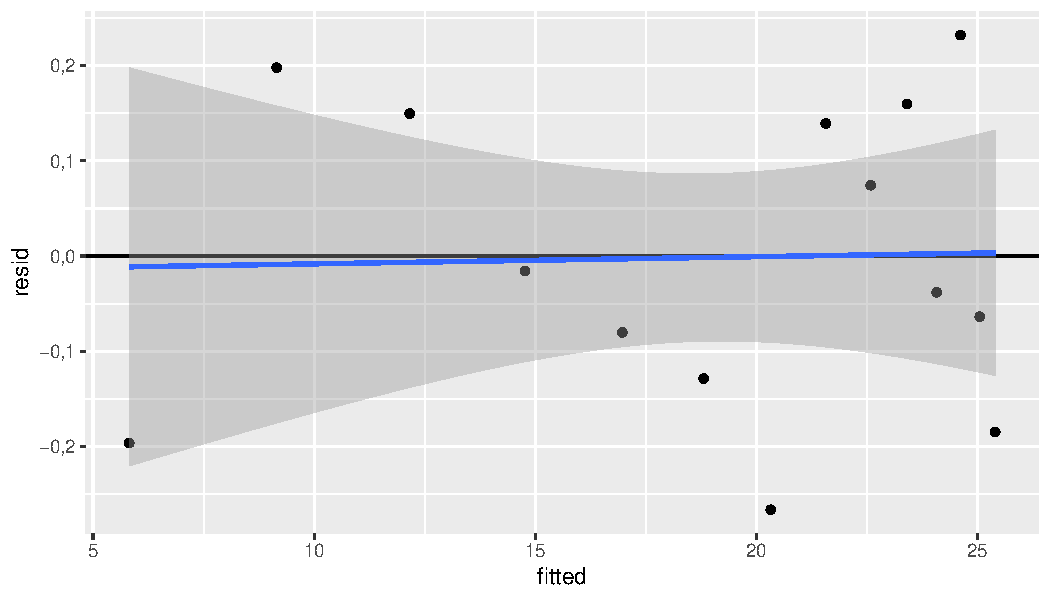
\includegraphics[width=0.8\linewidth]{_main_files/figure-latex/unnamed-chunk-60-1} \caption{Lineaarne regressioon}\label{fig:unnamed-chunk-60}
\end{figure}

Järgnevalt käsu selgitus:

\begin{itemize}
\item
  \texttt{ggplot(andmed,\ aes(x\ =\ d,\ y\ =\ h))}: See algatab ggplot-objekti, määrates andmestiku (data) ja esteetilised vastavused. See tähendab, et andmestiku veerg \texttt{d} vastendatakse x-teljega ja veerg \texttt{h} y-teljega.
\item
  \texttt{stat\_poly\_line()}: See lisab graafikule polünoomilise regressioonijoone. Vaikimisi kasutab see lineaarset mudelit (astmega 1), kuid seda saab muuta, kasutades argumenti \texttt{formula}. Näiteks \texttt{stat\_poly\_line(formula\ =\ y\ \textasciitilde{}\ x\^{}2)} lisaks graafikule ruutvõrrandi.
\item
  \texttt{stat\_poly\_eq(use\_label(c("eq",\ "R2")))}: See lisab graafikule polünoomilise regressioonivõrrandi ja R-ruudu väärtuse. \texttt{use\_label()} funktsiooniga saab määrata, milliseid tunnuseid kuvatakse. Antud juhul kuvatakse võrrand (\texttt{eq}) ja R-ruut (\texttt{R2}).
\item
  \texttt{geom\_point()}: See lisab graafikule punktid, mis tähistavad andmepunkte.
\item
  \texttt{xlim(c(10,\ 40))}: See seab x-telje piirid vahemikku 10 kuni 40.
\item
  \texttt{ylim(c(10,\ 40))}: See seab y-telje piirid vahemikku 10 kuni 40.
\end{itemize}

\begin{Shaded}
\begin{Highlighting}[]
\CommentTok{\# Näide R keskkonnas}
\FunctionTok{ggplot}\NormalTok{(andmed, }\FunctionTok{aes}\NormalTok{(}\AttributeTok{x =}\NormalTok{ d, }\AttributeTok{y =}\NormalTok{ h)) }\SpecialCharTok{+}
  \FunctionTok{stat\_poly\_line}\NormalTok{(}\AttributeTok{formula =}\NormalTok{ y }\SpecialCharTok{\textasciitilde{}} \FunctionTok{log}\NormalTok{(x)) }\SpecialCharTok{+}
  \FunctionTok{stat\_poly\_eq}\NormalTok{(}\AttributeTok{formula =}\NormalTok{ y }\SpecialCharTok{\textasciitilde{}} \FunctionTok{log}\NormalTok{(x), }\FunctionTok{use\_label}\NormalTok{(}\FunctionTok{c}\NormalTok{(}\StringTok{"eq"}\NormalTok{, }\StringTok{"R2"}\NormalTok{))) }\SpecialCharTok{+}
  \FunctionTok{geom\_point}\NormalTok{() }\SpecialCharTok{+}
  \FunctionTok{xlim}\NormalTok{(}\FunctionTok{c}\NormalTok{(}\DecValTok{10}\NormalTok{, }\DecValTok{40}\NormalTok{)) }\SpecialCharTok{+} \FunctionTok{ylim}\NormalTok{(}\FunctionTok{c}\NormalTok{(}\DecValTok{10}\NormalTok{, }\DecValTok{40}\NormalTok{))}
\end{Highlighting}
\end{Shaded}

\begin{figure}
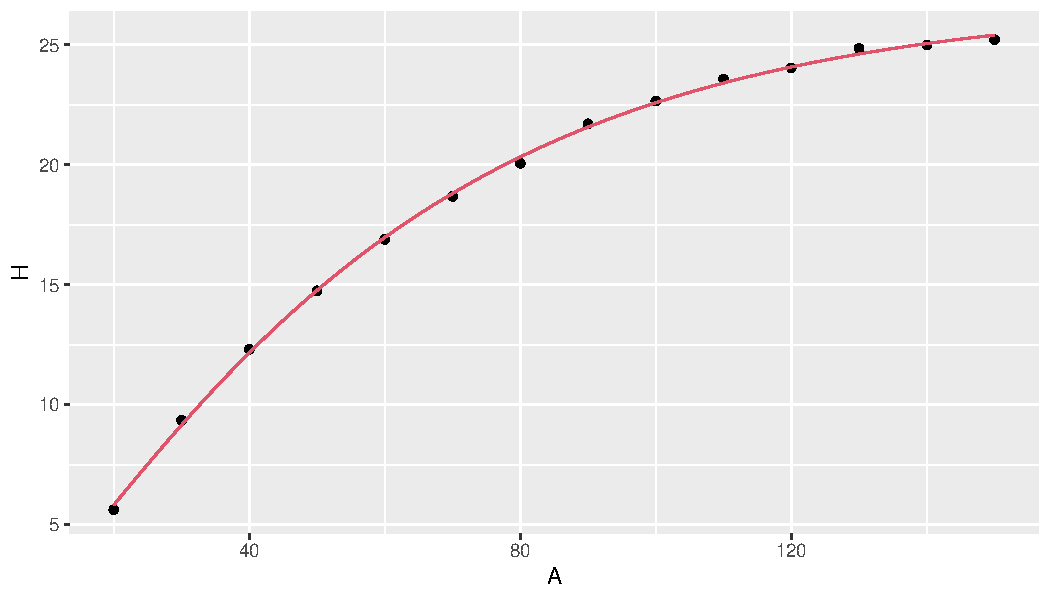
\includegraphics[width=0.8\linewidth]{_main_files/figure-latex/unnamed-chunk-61-1} \caption{Lineaarne regressioon argumenttunnuse logistilise teisendusega}\label{fig:unnamed-chunk-61}
\end{figure}

R-is on võimalik lihtalt lisada mudelisse täiendavad tunnuseid, mis arvutakse otse mudeli arvutamise käigus ning seetõttu ei ole vajalik eraldi eelnevalt täiendavat tunnust välja arvutada. Funktsiooniga \texttt{I()} saab luua uusi tunnuseid olemasolevate tunnuste põhjal. Uus tunnus arvutatakse iga andmerea jaoks mudeli arvutamise käigus.

Järgnevas näites on muudetud mudelit: \texttt{lm(h\ \textasciitilde{}\ log(d)+I(pl\ ==\ "MA"),\ data\ =\ andmed)}

\begin{itemize}
\tightlist
\item
  \textbf{\texttt{log(d)}}: Funktsioon \texttt{log()} arvutab \texttt{d} naturaallogaritmi, mis aitab lineariseerida seost diameetri ja kõrguse vahel.
\item
  \textbf{\texttt{I(pl\ ==\ "MA")}}: See on teine sõltumatu tunnus, mis luuakse jooksvalt funktsiooni \texttt{I()} abil. See on loogiline tunnus, mis on \texttt{TRUE}, kui tunnus \texttt{pl} väärtus on ``MA'' , ja \texttt{FALSE} vastasel juhul. Sisuliselt lisab see mudelisse teavet selle kohta, kas puu on mänd. Arvutustes kasutatakse antud tunnust vastavalt 1 või 0 väärtusena.
\end{itemize}

\begin{Shaded}
\begin{Highlighting}[]
\CommentTok{\# Näide R keskkonnas}
\CommentTok{\# täiendatud argumenttunnustega regressioon}
\FunctionTok{summary}\NormalTok{(lm\_model\_pl }\OtherTok{\textless{}{-}} \FunctionTok{lm}\NormalTok{(h }\SpecialCharTok{\textasciitilde{}} \FunctionTok{log}\NormalTok{(d)}\SpecialCharTok{+}\FunctionTok{I}\NormalTok{(pl }\SpecialCharTok{==} \StringTok{"MA"}\NormalTok{), }\AttributeTok{data =}\NormalTok{ andmed))}
\end{Highlighting}
\end{Shaded}

\begin{verbatim}

Call:
lm(formula = h ~ log(d) + I(pl == "MA"), data = andmed)

Residuals:
   Min     1Q Median     3Q    Max 
-2,169 -0,857  0,048  0,665  3,421 

Coefficients:
                  Estimate Std. Error t value Pr(>|t|)    
(Intercept)         -3,583      2,725   -1,31    0,195    
log(d)               8,924      0,872   10,24  3,2e-13 ***
I(pl == "MA")TRUE   -0,978      0,430   -2,27    0,028 *  
---
Signif. codes:  0 '***' 0,001 '**' 0,01 '*' 0,05 '.' 0,1 ' ' 1

Residual standard error: 1,27 on 44 degrees of freedom
Multiple R-squared:  0,707, Adjusted R-squared:  0,694 
F-statistic: 53,2 on 2 and 44 DF,  p-value: 1,81e-12
\end{verbatim}

Antud juhul on näha, et mänd on teistest statistiliselt oluliselt erinev.

\subsection{Lineaarne regressioon MS Exceli keskkonnas}\label{lineaarne-regressioon-ms-exceli-keskkonnas}

MS Exceli keskkonnas saab lineaarse regressiooni parameetreid arvutada mitmel viisil.

\begin{itemize}
\tightlist
\item
  Kui argumenttunnuseid on vaid üks, siis saab kasutada funktsioone \texttt{intercept()} ja \texttt{slope()}.
\item
  Kui argumenttunnuseid on mitu (või ka ainult üks), siis saab kasutada funktsiooni \texttt{linest()}, mis annab tulemuseks juba ka täpsemad mudeli parameetrite hinnangud.
\item
  Ühe ja mitme argumenttunnuse puhul saab kasutada \emph{Analysis Toolpak} protseduuri \emph{Regression}.
\end{itemize}

Avame faili \href{data/naited.xlsx}{naited.xlsx} töölehel ``linreg'', kus on samad andmed nagu ``prt\_andmed'', aga sellel on juba välja filtreeritud ainult mudelpuude andmed. MS Exceli keskkonnas on üldiselt vajalik filtreeritud andmed viia eraldi tabelisse, et regressiooni käigus muid andmeid ei kasutataks.

\emph{Analysis Toolpak} abil regressioonanalüüsi tegemiseks tuleb menüüs ``Andmed'' valida ``Data Analysis'', mis järel avaneb analüüsivahendite aken.

\begin{figure}
\centering
\pandocbounded{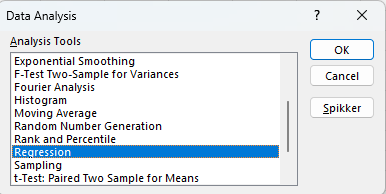
\includegraphics[keepaspectratio]{pildid/ms_excel_regression_step_1.png}}
\caption{Data Analysis aken MS Excelis.}
\end{figure}

\begin{figure}
\centering
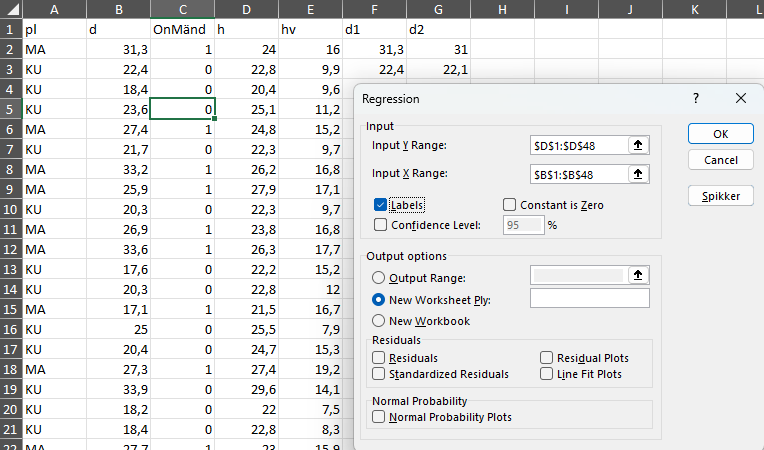
\includegraphics[width=0.8\linewidth,height=\textheight,keepaspectratio]{pildid/ms_excel_regression_step_2.png}
\caption{Regressioonanalüüsi aken MS Excelis.}
\end{figure}

Kordame samasugust analüüsi ka MS Exceli keskkonnas nagu R-is, arvutame diameetrist naturaallogaritmi funktsiooniga \texttt{ln()} ning kasutame \texttt{OnMänd} tunnust.

\begin{figure}
\centering
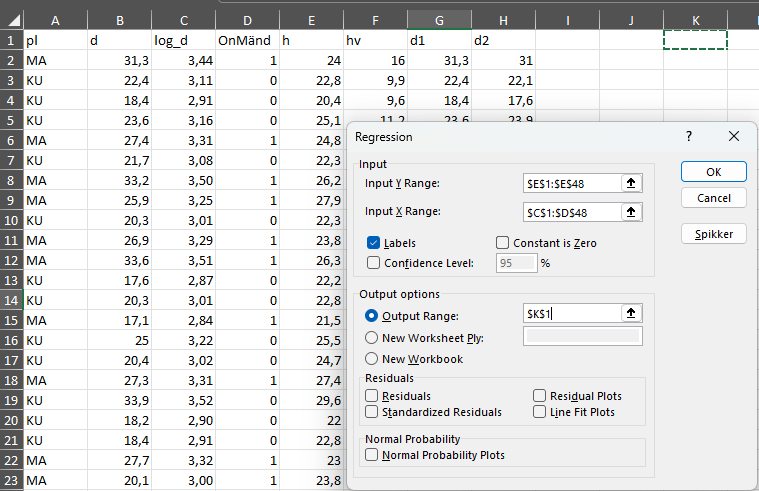
\includegraphics[width=0.8\linewidth,height=\textheight,keepaspectratio]{pildid/ms_excel_regression_step_3.png}
\caption{Regressioonanalüüs kahe tunnuse alusel.}
\end{figure}

\clearpage

Table: Lineaarse regressiooni tulemus MS Excelis.

\textbf{SUMMARY OUTPUT}

\begin{longtable}[]{@{}lr@{}}
\toprule\noalign{}
\textbf{Regression Statistics} & \\
\midrule\noalign{}
\endhead
\bottomrule\noalign{}
\endlastfoot
Multiple R & 0,841 \\
R Square & 0,707 \\
Adjusted R Square & 0,694 \\
Standard Error & 1,268 \\
Observations & 47 \\
\end{longtable}

\textbf{ANOVA}

\begin{longtable}[]{@{}
  >{\raggedright\arraybackslash}p{(\linewidth - 10\tabcolsep) * \real{0.1852}}
  >{\raggedleft\arraybackslash}p{(\linewidth - 10\tabcolsep) * \real{0.1111}}
  >{\raggedleft\arraybackslash}p{(\linewidth - 10\tabcolsep) * \real{0.1296}}
  >{\raggedleft\arraybackslash}p{(\linewidth - 10\tabcolsep) * \real{0.1111}}
  >{\raggedleft\arraybackslash}p{(\linewidth - 10\tabcolsep) * \real{0.1296}}
  >{\raggedleft\arraybackslash}p{(\linewidth - 10\tabcolsep) * \real{0.3333}}@{}}
\toprule\noalign{}
\begin{minipage}[b]{\linewidth}\raggedright
\end{minipage} & \begin{minipage}[b]{\linewidth}\raggedleft
\textbf{df}
\end{minipage} & \begin{minipage}[b]{\linewidth}\raggedleft
\textbf{SS}
\end{minipage} & \begin{minipage}[b]{\linewidth}\raggedleft
\textbf{MS}
\end{minipage} & \begin{minipage}[b]{\linewidth}\raggedleft
\textbf{F}
\end{minipage} & \begin{minipage}[b]{\linewidth}\raggedleft
\textbf{Significance F}
\end{minipage} \\
\midrule\noalign{}
\endhead
\bottomrule\noalign{}
\endlastfoot
Regression & 2 & 171,139 & 85,570 & 53,191 & 0,000 \\
Residual & 44 & 70,783 & 1,609 & & \\
Total & 46 & 241,922 & & & \\
\end{longtable}

\begin{longtable}[]{@{}
  >{\raggedright\arraybackslash}p{(\linewidth - 8\tabcolsep) * \real{0.1667}}
  >{\raggedleft\arraybackslash}p{(\linewidth - 8\tabcolsep) * \real{0.2424}}
  >{\raggedleft\arraybackslash}p{(\linewidth - 8\tabcolsep) * \real{0.2727}}
  >{\raggedleft\arraybackslash}p{(\linewidth - 8\tabcolsep) * \real{0.1515}}
  >{\raggedleft\arraybackslash}p{(\linewidth - 8\tabcolsep) * \real{0.1667}}@{}}
\toprule\noalign{}
\begin{minipage}[b]{\linewidth}\raggedright
\end{minipage} & \begin{minipage}[b]{\linewidth}\raggedleft
\textbf{Coefficients}
\end{minipage} & \begin{minipage}[b]{\linewidth}\raggedleft
\textbf{Standard Error}
\end{minipage} & \begin{minipage}[b]{\linewidth}\raggedleft
\textbf{t Stat}
\end{minipage} & \begin{minipage}[b]{\linewidth}\raggedleft
\textbf{P-value}
\end{minipage} \\
\midrule\noalign{}
\endhead
\bottomrule\noalign{}
\endlastfoot
Intercept & -3,5829 & 2,7247 & -1,3150 & 0,1953 \\
log\_d & 8,9235 & 0,8718 & 10,2358 & 0,0000 \\
OnMänd & -0,9776 & 0,4300 & -2,2737 & 0,0279 \\
\end{longtable}

\subsection{Regressioonanalüüsi tulemuste tõlgendamine}\label{regressioonanaluxfcuxfcsi-tulemuste-tuxf5lgendamine}

Lineaarse regressioonimudeli kokkuvõte sisaldab mitmeid olulisi statistilisi näitajaid, mis aitavad hinnata mudeli sobivust andmetele.

Determinatsioonikordaja, tuntud ka kui \(R^2\) (R-ruut), on statistiline mõõdik, mida kasutatakse lineaarse regressiooni kontekstis, et hinnata, kui suures ulatuses argumenttunnuse variatsioon on seletatav sõltumatute tunnuste abil mudelis. \(R^2\) väärtus varieerub vahemikus 0 kuni 1, kus 0 tähendab, et mudel ei seleta argumenttunnuse variatsiooni üldse, samas kui 1 tähendab, et mudel seletab argumenttunnuse variatsiooni täielikult.

\(R^2\) arvutamiseks kasutatakse järgmist valemit:

\[ R^2 = 1 - \frac{\text{SS}_\text{res}}{\text{SS}_\text{tot}} \]

kus:

\begin{itemize}
\tightlist
\item
  \(\text{SS}_\text{res}\) on jääkide ruutude summa (residual sum of squares), mis mõõdab mudeli poolt seletamata variatsiooni.
\item
  \(\text{SS}_\text{tot}\) on kogu variatsiooni ruutude summa (total sum of squares), mis mõõdab argumenttunnuse variatsiooni võrreldes tema keskmisega.
\end{itemize}

\textbf{Kõrge \(R^2\) väärtus} (lähedane 1-le) näitab, et mudeli poolt seletatav variatsioon on suur, mis tähendab, et mudel sobib andmetele hästi. See viitab sellele, et suur osa argumenttunnuse variatsioonist on seletatav mudeli sõltumatute tunnustega.

\textbf{Madal \(R^2\) väärtus} (lähedane 0-le) näitab, et mudel seletab argumenttunnuse variatsioonist väikese osa, mis tähendab, et mudeli sobivus andmetele on kehv. See võib viidata sellele, et mudelis kasutatavad sõltumatud tunnused ei ole sõltuva tunnuse variatsiooni seletamisel tõhusad.

Oluline on mõista, et kuigi \(R^2\) on kasulik mõõdik mudeli sobivuse hindamisel, ei tähenda kõrge \(R^2\) automaatselt, et mudel on õige või et sõltumatud tunnusd põhjustavad argumenttunnuse käitumist. Samuti ei pruugi madal \(R^2\) alati tähendada mudeli ebatõhusust, eriti keerukamate või mittelineaarsete suhete puhul. Lisaks tuleks mudeli hindamisel arvesse võtta ka muid tegureid, nagu mudeli tõlgendatavus, sõltumatute tunnuste olulisus ja korrigeeritud \(R^2\).

Lineaarse regressioonimudeli \textbf{nihutamata hinnang}, tuntud ka kui korrigeeritud \(R^2\) (inglise keeles ``adjusted \(R^2\)''), on statistiline mõõdik, mida kasutatakse mudeli seletusvõime hindamiseks, võttes arvesse mudeli sõltumatute tunnuste arvu. Erinevalt lihtsast \(R^2\)-st, mis mõõdab, kui suur osa argumenttunnuse variatsioonist on seletatav mudeli abil, arvestab korrigeeritud \(R^2\) mudeli keerukust, arvestab mudeli liigsete sõltumatute tunnuste lisamise eest. See on oluline, kuna mudelisse liiga palju tunnusid lisades võib \(R^2\) väärtus eksitavalt tõusta, viidates paremale mudeli sobivusele, kuigi tegelikult võivad lisatud tunnusd olla statistiliselt mitteolulised.

Korrigeeritud \(R^2\) arvutatakse järgmise valemi järgi:

\[ R^2_{\text{adj}} = 1 - \left( \frac{(1 - R^2)(n - 1)}{n - k - 1} \right) \]

kus:

\begin{itemize}
\tightlist
\item
  \(R^2\) on mudeli lihtne determinatsioonikoefitsient,
\item
  \(n\) on vaatluste arv,
\item
  \(k\) on sõltumatute tunnuste arv mudelis.
\end{itemize}

Valemist nähtub, et \(R^2_{\text{adj}}\) väheneb, kui lisatakse tunnusid, mis ei paranda mudeli seletusvõimet proportsionaalselt nende arvuga. Seega, erinevalt lihtsast \(R^2\)-st, pakub korrigeeritud \(R^2\) ausamat hinnangut mudeli sobivusele, eriti kui võrrelda mudeleid, mis sisaldavad erinevat arvu sõltumatuid tunnusid. Korrigeeritud \(R^2\) on eriti kasulik mudelite võrdlemisel ja mudeli valimisel, aidates vältida ülemudelitamist ja eelistades mudelit, mis annab parima tasakaalu seletusvõime ja keerukuse vahel.

\begin{itemize}
\item
  P-väärtused näitavad, kas argumenttunnus on statistiliselt oluline mudelis. Kui P-väärtus on väiksem kui 0,05, siis võib järeldada, et argumenttunnus mõjutab oluliselt sõltuvat tunnust.
\item
  Regressioonikordaja väärtused annavad teavet sõltumatute tunnuste mõju kohta sõltuvale tunnusle.
\end{itemize}

Kokkuvõttes aitab väljund mõista, kuidas mudel sobitub andmetega ja millist infot see pakub sõltuvate ja sõltumatute tunnuste seoste kohta.

\subsection{Homoskedastilisuse testimine}\label{homoskedastilisuse-testimine}

Statistilise regressioonimudeli kontekstis viitab homoskedastiivsus olukorrale, kus jääkliikmete (ehk mudeli veatermini) dispersioon on konstantne sõltumata seletavate muutujate väärtustest. See tähendab, et mudeli ennustusvead on ühtlase hajuvusega kogu vaadeldava andmevahemiku ulatuses, ega ole süstemaatiliselt seotud ennustatud väärtustega. Homoskedastiivsus on kriitiline eeldus mitmetes statistilistes meetodites, eriti vähimruutude meetodil baseeruva lineaarse regressiooni puhul. Selle eelduse rikkumine, tuntud kui heteroskedastiivsus, võib moonutada mudeli parameetrite hinnanguid, viies ebatäpsete usaldusvahemike ja potentsiaalselt vigaste järeldusteni hüpoteeside testimisel.

On mitmeid viise, kuidas testida, kas andmetes esineb homoskedastiivsust:

\begin{enumerate}
\def\labelenumi{\arabic{enumi}.}
\tightlist
\item
  \textbf{Visuaalne analüüs:} Lihtsaim viis on vaadata jääkliikmete graafikut seletavate muutujate või ennustatud väärtuste suhtes. Kui jääkliikmed on ühtlaselt hajunud nulljoone ümber, on homoskedastiivsus tõenäoline. Kui tekib mingi muster (näiteks koonusekujuline hajumine), on tõenäoline heteroskedastiivsus.
\item
  \textbf{Formaliseeritud testid:} On olemas mitmed statistilised testid, näiteks Breusch-Pagani test ja White'i test, mis testivad heteroskedastiivsust formaalselt. Need testid kontrollivad, kas jääkliikmete dispersioon on seotud seletavate muutujatega.
\item
  \textbf{Robustsed meetodid:} Kui andmetes esineb heteroskedastiivsust, võib kasutada robustseid regressioonimeetodeid, mis on vähem tundlikud heteroskedastiivsuse suhtes.
\end{enumerate}

\begin{Shaded}
\begin{Highlighting}[]
\CommentTok{\# Näide R keskkonnas}
\FunctionTok{plot}\NormalTok{(lm\_model, }\AttributeTok{which=}\DecValTok{1}\NormalTok{, }\AttributeTok{main =} \StringTok{""}\NormalTok{) }
\end{Highlighting}
\end{Shaded}

\begin{figure}
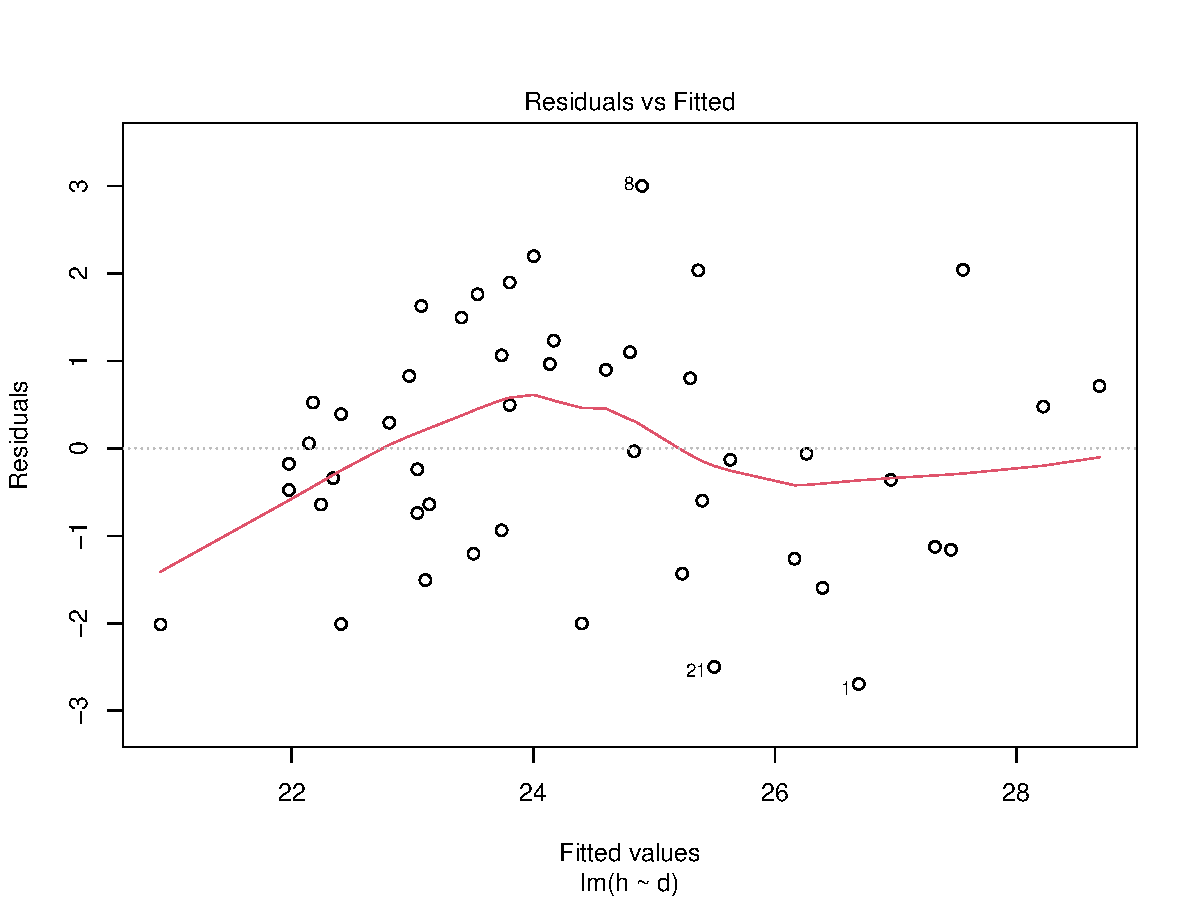
\includegraphics[width=0.8\linewidth]{_main_files/figure-latex/unnamed-chunk-63-1} \caption{Jäägid vs prognoositud väärtus}\label{fig:unnamed-chunk-63}
\end{figure}

Lineaarse mudeli homoskedastilisuse testimiseks saab kasutada Breush-Pagan või White'i testi. Need testid hindavad, kas jääkide varieeruvus on seotud sõltumatute tunnustega ning kas see varieeruvus on ühtlane.

\begin{Shaded}
\begin{Highlighting}[]
\CommentTok{\# Näide R keskkonnas}
\NormalTok{lmtest}\SpecialCharTok{::}\FunctionTok{bptest}\NormalTok{(lm\_model)}
\end{Highlighting}
\end{Shaded}

\begin{verbatim}

    studentized Breusch-Pagan test

data:  lm_model
BP = 0,9, df = 1, p-value = 0,4
\end{verbatim}

Paketi \texttt{lmtest} funktsioon \texttt{bptest()} testib regressioonimudeli jääkide heteroskedastsuse olemasolu. See tähendab, et jääkide varieeruvus ei ole konstantne üle kõigi sõltumatute tunnuste väärtuste ning võib tekitada probleeme statistiliste hüpoteeside testimisel.

Testi tulemusi võib lugeda järgmiselt:

\begin{itemize}
\tightlist
\item
  Nullhüpotees (H0): jääkide varieeruvus on konstantne (st heteroskedastsust ei esine).
\item
  Alternatiivhüpotees (H1): jääkide varieeruvus ei ole konstantne (st heteroskedastsus esineb).
\end{itemize}

Testist saadav p-väärtus aitab hinnata, kas on piisavalt tõendeid, et lükata ümber nullhüpotees heteroskedastsuse puudumise kohta. Väike p-väärtus (\textless0,05) viitab sellele, et saame nullhüpoteesi ümber lükata ja järeldada, et heteroskedastsust esineb.

\subsection{Jääkide normaalsuse test}\label{juxe4uxe4kide-normaalsuse-test}

Üks oluline eeldus, mida lineaarses regressioonis kasutatakse, on see, et mudeli jäägid vastaksid normaaljaotusele. Normaaljaotus tähendab, et andmete jaotus on sümmeetriline ning keskmise jaotusega. Kui jäägid on normaaljaotusele lähedased, siis on regressioonimudeli ennustused usaldusväärsemad ja täpsemad. Paljud statistilised testid eeldavad, et andmed vastavad normaaljaotusele. Kui jäägid ei vasta normaaljaotusele, võivad testide tulemused olla ebatäpsed või valed. Normaaljaotuse eeldustele mitte vastamine võib viidata sellele, et mudel ei sobi antud andmetele hästi ning on vajalik leida alternatiivseid mudeleid.

Normaliseeritud jääkide graafik on üks viis, kuidas hinnata, kas jäägid vastavad normaaljaotusele. See graafik aitab visualiseerida, kas jäägid on juhuslikult hajutatud ümber nulli ja kas nende jaotus on ligilähedane normaaljaotusele.

\begin{Shaded}
\begin{Highlighting}[]
\CommentTok{\# Näide R keskkonnas}

\FunctionTok{ggplot}\NormalTok{(lm\_model, }\FunctionTok{aes}\NormalTok{(}\AttributeTok{x =}\NormalTok{ .fitted, }\AttributeTok{y =}\NormalTok{ .resid)) }\SpecialCharTok{+}
  \FunctionTok{geom\_point}\NormalTok{() }\SpecialCharTok{+}
  \FunctionTok{geom\_hline}\NormalTok{(}\AttributeTok{yintercept =} \DecValTok{0}\NormalTok{)}\SpecialCharTok{+}
  \FunctionTok{geom\_smooth}\NormalTok{(}\AttributeTok{method =} \StringTok{"gam"}\NormalTok{, }\AttributeTok{formula =}\NormalTok{ y }\SpecialCharTok{\textasciitilde{}} \FunctionTok{s}\NormalTok{(x))  }\CommentTok{\# Lisab sujuva joone GAM mudeli abil}
\end{Highlighting}
\end{Shaded}

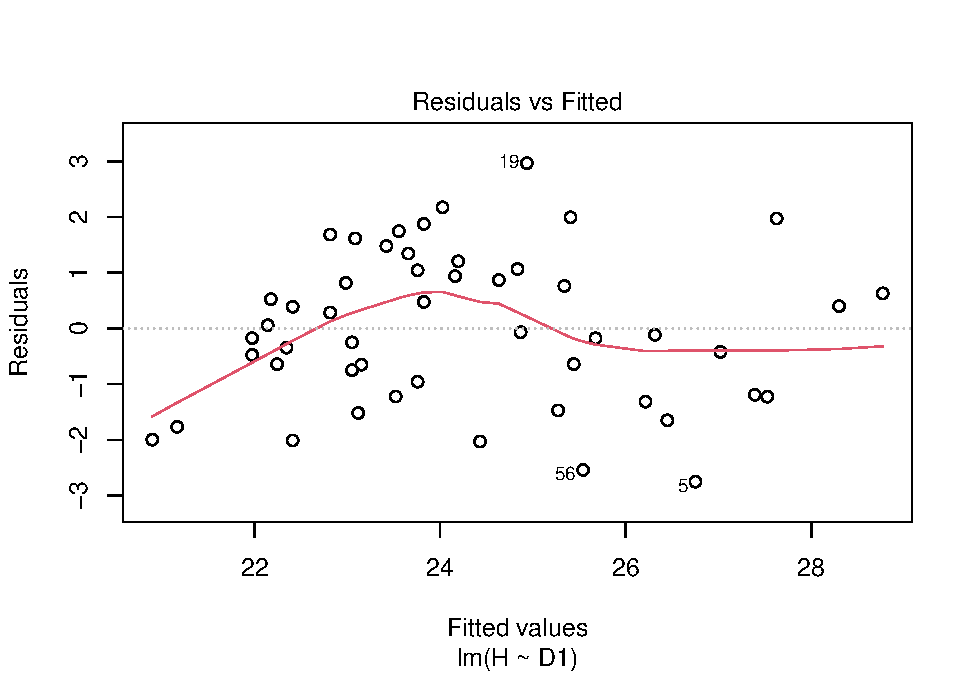
\includegraphics[width=0.8\linewidth]{_main_files/figure-latex/unnamed-chunk-65-1}
Koodi selgitus:

\textbf{\texttt{ggplot(lm\_model,\ aes(x\ =\ .fitted,\ y\ =\ .resid))}}

\begin{itemize}
\tightlist
\item
  See käsk loob aluse graafikule ggplot2 paketiga.
\item
  \texttt{lm\_model} määrab andmeallika, milleks on lineaarne mudel.
\item
  \texttt{aes(x\ =\ .fitted,\ y\ =\ .resid)} määrab x-teljele mudeli sobitatud väärtused (.fitted) ja y-teljele jääkväärtused (.resid).
\end{itemize}

\textbf{\texttt{geom\_point()}}

\begin{itemize}
\tightlist
\item
  See lisab graafikule punktid, mis esindavad iga andmepunkti jääki ja sobitatud väärtust.
\end{itemize}

\textbf{\texttt{geom\_hline(yintercept\ =\ 0)}}

\begin{itemize}
\tightlist
\item
  See lisab horisontaalse joone y-telje väärtusel 0. See joon aitab visuaalselt hinnata jääkide jaotust - ideaalses mudelis peaksid punktid jaotuma ühtlaselt joone ümber.
\end{itemize}

\textbf{\texttt{geom\_smooth(method\ =\ "gam",\ formula\ =\ y\ \textasciitilde{}\ s(x))}}

\begin{itemize}
\tightlist
\item
  See lisab graafikule sujuva joone, mis on arvutatud GAM mudeli (Generalized Additive Model) abil.
\item
  \texttt{method\ =\ "gam"} määrab joone arvutamise meetodiks GAM.
\item
  \texttt{formula\ =\ y\ \textasciitilde{}\ s(x)} määrab mudeli valemi, kus y (jääkväärtused) on seotud x-i (sobitatud väärtused) sujuva funktsiooniga s(x).
\end{itemize}

\textbf{Kokkuvõtteks:}

Kood genereerib diagnostilise graafiku, mis aitab hinnata lineaarse mudeli sobivust andmetega. Jääkide jaotus 0-joone ümber ja sujuva joone kuju annavad informatsiooni mudeli eelduste (nt homoskedastsus ja lineaarsus) täidetuse kohta.

Samuti saab vaadata jääkide jagunemist tihedusfunktsiooni abil koostatud graafikul.

\begin{Shaded}
\begin{Highlighting}[]
\CommentTok{\# Näide R keskkonnas}

\FunctionTok{ggplot}\NormalTok{(lm\_model, }\FunctionTok{aes}\NormalTok{(}\AttributeTok{x =}\NormalTok{ .resid)) }\SpecialCharTok{+}
  \FunctionTok{geom\_density}\NormalTok{()}
\end{Highlighting}
\end{Shaded}

\begin{figure}
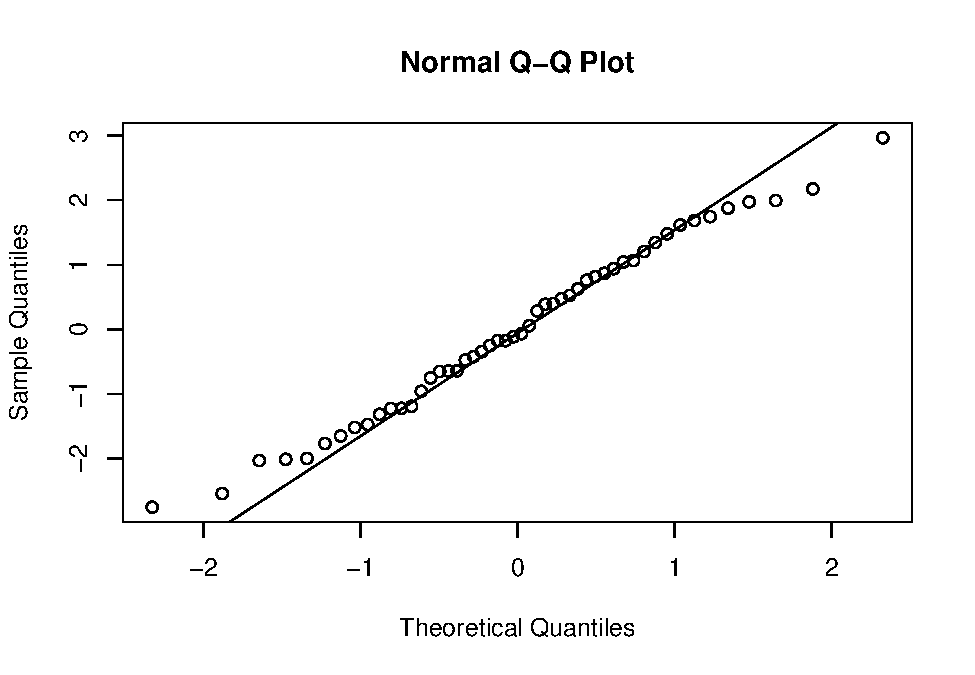
\includegraphics[width=0.8\linewidth]{_main_files/figure-latex/unnamed-chunk-66-1} \caption{Jääkide tihedusfunktsioon}\label{fig:unnamed-chunk-66}
\end{figure}

Sellise protseduuri abil saad hinnata, kui hästi sobib loodud lineaarne regressioonimudel andmetele ning kas jääkide jaotus vastab normaalsuse eeldusele.

\begin{Shaded}
\begin{Highlighting}[]
\CommentTok{\# Näide R keskkonnas}
\CommentTok{\# ANOVA}
\FunctionTok{anova}\NormalTok{(lm\_model)}
\end{Highlighting}
\end{Shaded}

\begin{verbatim}
Analysis of Variance Table

Response: h
          Df Sum Sq Mean Sq F value  Pr(>F)    
d          1  158,5   158,5    85,5 5,7e-12 ***
Residuals 45   83,4     1,9                    
---
Signif. codes:  0 '***' 0,001 '**' 0,01 '*' 0,05 '.' 0,1 ' ' 1
\end{verbatim}

\begin{Shaded}
\begin{Highlighting}[]
\FunctionTok{confint}\NormalTok{(lm\_model)}
\end{Highlighting}
\end{Shaded}

\begin{verbatim}
            2,5 % 97,5 %
(Intercept) 14,49 18,099
d            0,26  0,405
\end{verbatim}

\subsection{Multikollineaarsus}\label{multikollineaarsus}

Lineaarses regressioonis tähistab multikollineaarsus olukorda, kus kaks või enam sõltumatut tunnust (selgitajat) on omavahel tugevalt seotud või korreleerunud. See tähendab, et ühe selgitaja väärtusi saab suure täpsusega ennustada teiste selgitajate väärtuste põhjal. Multikollineaarsus võib olla probleemiks, sest:

Mõjutab koefitsientide hinnangute täpsust: multikollineaarsus suurendab koefitsientide hinnangute varieeruvust, mis muudab need ebastabiilseks. Väiksed muudatused andmestikus võivad tuua kaasa suuri muutusi koefitsientide hinnangutes, muutes mudeli interpretatsiooni keeruliseks.

Raskendab tunnuste tähtsuse hindamist: kõrge multikollineaarsuse korral võib olla raske kindlaks teha, milline argumenttunnus mõjutab sõltuvat tunnust, sest statistilised testid ei pruugi olla usaldusväärsed. See võib viia oluliste tunnuste ebaõiglase kõrvalejätmiseni või ebaoluliste tunnuste mudelisse lisamiseni.

Vähendab mudeli interpretatsiooni selgust: kui argumenttunnused on omavahel tugevalt seotud, muutub mudeli interpretatsioon keerulisemaks, kuna keeruline on eristada iga tunnus unikaalset mõju argumenttunnusele .

Multikollineaarsuse tuvastamiseks lineaarses regressioonis kasutatakse tavaliselt järgmisi meetodeid:

\begin{itemize}
\tightlist
\item
  \textbf{Korrelatsioonimatriks}: Vaadeldakse sõltumatute tunnuste vahelisi korrelatsioonikoefitsiente. Kõrge korrelatsioon näitab võimalikku multikollineaarsust.
\item
  \textbf{Variance Inflation Factor (VIF)}: VIF mõõdab, kui palju tunnus variatiivsus suureneb multikollineaarsuse tõttu. Tavaliselt peetakse VIF väärtust üle 5 või 10 viitavaks tugevale multikollineaarsusele.
\item
  \textbf{Tolerants}: Tolerants on VIF-i pöördväärtus ja näitab, kui suur osa tunnus variatsioonist ei ole seletatav teiste mudeli tunnustega. Madal tolerants viitab multikollineaarsusele.
\end{itemize}

Multikollineaarsuse lahendamiseks võib kasutada mitmeid lähenemisviise, näiteks tunnuste eemaldamist mudelist, tunnuste kombineerimist või andmete transformeerimist. Samuti võib kasulikuks osutuda regulaarimismeetodite, nagu ridge regressioon või lasso regressioon, kasutamine, mis aitavad vähendada koefitsientide varieeruvust, karistades suuri koefitsiente.

Vaatame järgmist näidet, kus puude kõrgust ennustame mõlema diameetri alusel. Kui varasemalt oli näha, et üks diameeter on oluline, siis antud mudelid ei ole enam kumbki oluline, sest nende tunnuse vahel on korrelatsioon.

\begin{Shaded}
\begin{Highlighting}[]
\CommentTok{\# Näide R keskkonnas}
\FunctionTok{summary}\NormalTok{(lm.col }\OtherTok{\textless{}{-}} \FunctionTok{lm}\NormalTok{(h }\SpecialCharTok{\textasciitilde{}}\NormalTok{ d1 }\SpecialCharTok{+}\NormalTok{ d2, }\AttributeTok{data =}\NormalTok{ andmed))}
\end{Highlighting}
\end{Shaded}

\begin{verbatim}

Call:
lm(formula = h ~ d1 + d2, data = andmed)

Residuals:
   Min     1Q Median     3Q    Max 
-2,709 -0,893 -0,200  0,787  3,143 

Coefficients:
            Estimate Std. Error t value Pr(>|t|)    
(Intercept)  16,1390     0,8902   18,13   <2e-16 ***
d1           -0,0231     0,2431   -0,09     0,92    
d2            0,3643     0,2466    1,48     0,15    
---
Signif. codes:  0 '***' 0,001 '**' 0,01 '*' 0,05 '.' 0,1 ' ' 1

Residual standard error: 1,34 on 44 degrees of freedom
Multiple R-squared:  0,671, Adjusted R-squared:  0,656 
F-statistic:   45 on 2 and 44 DF,  p-value: 2,32e-11
\end{verbatim}

Tehes täiendavalt ANOVA, on näha, et diameeter, mis lineaarses regressioonimudelis ei olnud oluline, on dispersioonanalüüsi järgi peamine varieeruvuse kirjeldaja.

\begin{Shaded}
\begin{Highlighting}[]
\CommentTok{\# Näide R keskkonnas}
\FunctionTok{anova}\NormalTok{(lm.col)}
\end{Highlighting}
\end{Shaded}

\begin{verbatim}
Analysis of Variance Table

Response: h
          Df Sum Sq Mean Sq F value  Pr(>F)    
d1         1  158,5   158,5   87,73 4,8e-12 ***
d2         1    3,9     3,9    2,18    0,15    
Residuals 44   79,5     1,8                    
---
Signif. codes:  0 '***' 0,001 '**' 0,01 '*' 0,05 '.' 0,1 ' ' 1
\end{verbatim}

\begin{Shaded}
\begin{Highlighting}[]
\CommentTok{\# Arvutame VIF väärtuse multikollineaarsuse tuvastamiseks}
\FunctionTok{vif}\NormalTok{(lm.col)}
\end{Highlighting}
\end{Shaded}

\begin{verbatim}
d1 d2 
47 47 
\end{verbatim}

Kui VIF väärtus on üle 5, siis on tunnuste vahel tugev korrelatsioon, mida saame kontrollida ka korrelatsioonimaatriksiga.

\begin{Shaded}
\begin{Highlighting}[]
\CommentTok{\# Näide R keskkonnas}
\FunctionTok{cor}\NormalTok{(andmed[,}\FunctionTok{c}\NormalTok{(}\StringTok{"d1"}\NormalTok{,}\StringTok{"d2"}\NormalTok{)])}
\end{Highlighting}
\end{Shaded}

\begin{verbatim}
      d1    d2
d1 1,000 0,989
d2 0,989 1,000
\end{verbatim}

Sellest on näha, et need on tugevas korrelatsioonis (0,986). See mõjutab ka lineaarse regressiooni parameetrite arvutamist.

\section{Dispersioonanalüüs}\label{dispersioonanaluxfcuxfcs}

Mitmese regressioonanalüüsi korral on tegemist mudeliga, kus pidev funktsioontunnus avaldub pidevate argumenttunnuste lineaarkombinatsioonina. Dispersioonanalüüsi korral on tegemist mudelitega, kus funktsioontunnuseks on pidev tunnus, kuid argument-tunnused on diskreetsed (võivad olla nii arvulised kui ka mittearvulised). Dispersioon-analüüsi argumenttunnuseid nimetatakse faktoriteks. Ühefaktorilise dispersioonanalüüsi puhul uuritakse funktsioontunnuse sõltuvust ainult ühest faktorist. Faktori võimalikke väärtusi nimetatakse faktori tasemeteks.

Olgu üldkogum jaotatud mittelõikuvateks osadeks ehk rühmadeks faktori tasemete järgi. Öeldakse, et faktor X mõjub tunnusele Y, kui tunnuse Y keskväärtused eri rühmades on erinevad. Uurija käsutuses on valimi mõõtmisandmed, mille funktsioon-tunnuse rühmakeskmised tavaliselt erinevad. Dispersioonanalüüs on meetod, millega otsitakse vastust küsimusele, kas valimi rühmakeskmiste erinevus on põhjustatud uuritava faktori mõjust või valimi juhuslikkusest.

Dispersioonanalüüsi võimalused ja vahendid sõltuvad oluliselt valitud mudelist ja katsekorraldusest. Kui iga faktortunnuse igal tasemel on tehtud ühepalju mõõtmisi, nimetatakse mudelit tasakaalustatuks, vastasel juhul on tegemist tasakaalustamata mudeliga. Kui mõõtmisi on tehtud faktori kõigil võimalikel tasemetel, siis nimetatakse seda fikseeritud faktoriks. Kui faktortunnusel on palju erinevaid väärtusi ja mõõdetud tasemeid vaadeldakse juhusliku valimina faktori võimalike tasemete hulgast, siis nimetatakse seda juhuslikuks faktoriks. Järgnevalt käsitleme ainult fikseeritud faktoritega mudeleid.

\chapter{Mittelineaarne regressioon}\label{mittelineaarne-regressioon}

\textbf{Mittelineaarne regressioon} on statistiline meetod, mida kasutatakse sõltuva muutuja ja ühe või mitme sõltumatu muutuja vahelise mittelineaarse seose modelleerimiseks. Erinevalt lineaarsest regressioonist, mis eeldab sirgjoonelist seost, võimaldab mittelineaarne regressioon paindlikumaid seoseid, näiteks kõverjoonelisi, eksponentsiaalseid või logistilisi seoseid.

Metsanduses esineb sageli mittelineaarseid seoseid. Mittelineaarne regressioon võimaldab neid keerukaid seoseid täpsemalt modelleerida ja paremini mõista.

Mittelineaarne regressioonimudel kirjutatakse üldjuhul kujul:

\[Y = f(X, \beta) + \epsilon\]

kus:

\begin{itemize}
\tightlist
\item
  \textbf{Y} on sõltuv muutuja.
\item
  \textbf{X} on sõltumatu(te) muutuja(te) vektor.
\item
  \textbf{\(f(X, \beta)\)} on mittelineaarne funktsioon, mis kirjeldab seost X ja Y vahel.
\item
  \textbf{\(\beta\)} on mudeli parameetrite vektor, mida tuleb hinnata.
\item
  \textbf{\(\epsilon\)} on vealiige, mis esindab juhuslikku varieeruvust.
\end{itemize}

Mittelineaarse regressiooni parameetreid hinnatakse tavaliselt \textbf{vähimruutude meetodil}, kus otsitakse parameetrite väärtusi, mis minimeerivad mudeli ennustatud väärtuste ja tegelike väärtuste vaheliste ruutude summat. See on iteratiivne protsess, mis nõuab arvutitarkvara kasutamist.

\section{R}\label{r}

Näiteks, kui soovime R-is kasutada \texttt{nls()} mudelit, mis kirjeldab puu kõrgust sõltuvalt puu diameetrist, võime kasutada järgmist näidiskoodi.

\begin{Shaded}
\begin{Highlighting}[]
\CommentTok{\# Laadime peatükis kasutatavad paketid}
\FunctionTok{library}\NormalTok{(dplyr)}
\FunctionTok{library}\NormalTok{(readxl)}
\end{Highlighting}
\end{Shaded}

\begin{Shaded}
\begin{Highlighting}[]
\CommentTok{\# Laadime andmed sisse failist ning}
\CommentTok{\# filtreerime välja puud, mille h \textgreater{} 0}
\NormalTok{andmed }\OtherTok{\textless{}{-}} \FunctionTok{read\_excel}\NormalTok{(}\StringTok{"data/naited.xlsx"}\NormalTok{,}\StringTok{"prt\_andmed"}\NormalTok{) }\SpecialCharTok{\%\textgreater{}\%} \FunctionTok{filter}\NormalTok{(h }\SpecialCharTok{\textgreater{}} \DecValTok{0}\NormalTok{)}
\end{Highlighting}
\end{Shaded}

\begin{Shaded}
\begin{Highlighting}[]
\CommentTok{\# Määratleme mudeli funktsioon}
\NormalTok{puu\_mudel }\OtherTok{\textless{}{-}} \ControlFlowTok{function}\NormalTok{(D, a, b, c) \{}
 \FloatTok{1.3} \SpecialCharTok{+}\NormalTok{ a }\SpecialCharTok{*}\NormalTok{ (D }\SpecialCharTok{/}\NormalTok{ (D }\SpecialCharTok{+}\NormalTok{ b))}\SpecialCharTok{\^{}}\NormalTok{c}
\NormalTok{\}}
\end{Highlighting}
\end{Shaded}

\begin{Shaded}
\begin{Highlighting}[]
\CommentTok{\# Omista algväärtused parameetritele}
\NormalTok{alg\_param }\OtherTok{\textless{}{-}} \FunctionTok{list}\NormalTok{(}\AttributeTok{a =} \DecValTok{1}\NormalTok{, }\AttributeTok{c =} \FloatTok{0.5}\NormalTok{)}
\end{Highlighting}
\end{Shaded}

\begin{Shaded}
\begin{Highlighting}[]
\CommentTok{\# Sobita mudel andmetele}
\NormalTok{mudel }\OtherTok{\textless{}{-}} \FunctionTok{nls}\NormalTok{(h }\SpecialCharTok{\textasciitilde{}} \FunctionTok{puu\_mudel}\NormalTok{(d, a, }\DecValTok{5}\NormalTok{, c), }\AttributeTok{data =}\NormalTok{ andmed, }\AttributeTok{start =}\NormalTok{ alg\_param)}
\end{Highlighting}
\end{Shaded}

\begin{Shaded}
\begin{Highlighting}[]
\CommentTok{\# Vaata mudeli kokkuvõtet}
\FunctionTok{summary}\NormalTok{(mudel)}
\end{Highlighting}
\end{Shaded}

\begin{verbatim}

Formula: h ~ puu_mudel(d, a, 5, c)

Parameters:
  Estimate Std. Error t value Pr(>|t|)    
a   34,341      1,430   24,01  < 2e-16 ***
c    2,056      0,216    9,51  2,4e-12 ***
---
Signif. codes:  0 '***' 0,001 '**' 0,01 '*' 0,05 '.' 0,1 ' ' 1

Residual standard error: 1,32 on 45 degrees of freedom

Number of iterations to convergence: 7 
Achieved convergence tolerance: 1,14e-07
\end{verbatim}

Esitame selle kohta ka graafiku, millele lisame mudeli joone funktsioonidega \texttt{curve()} ja \texttt{predict()}, milles kasutame loodud mudeli objekti.

\begin{Shaded}
\begin{Highlighting}[]
\FunctionTok{plot}\NormalTok{(h}\SpecialCharTok{\textasciitilde{}}\NormalTok{d, andmed, }\AttributeTok{ylim=}\FunctionTok{c}\NormalTok{(}\DecValTok{10}\NormalTok{, }\DecValTok{35}\NormalTok{), }\AttributeTok{xlim =} \FunctionTok{c}\NormalTok{(}\DecValTok{10}\NormalTok{, }\DecValTok{40}\NormalTok{))}
\FunctionTok{curve}\NormalTok{(}\FunctionTok{predict}\NormalTok{(mudel, }\FunctionTok{data.frame}\NormalTok{(}\AttributeTok{d =}\NormalTok{ x)), }\DecValTok{10}\NormalTok{, }\DecValTok{40}\NormalTok{, }\AttributeTok{add=}\NormalTok{T, }\AttributeTok{col =} \DecValTok{2}\NormalTok{)}
\end{Highlighting}
\end{Shaded}

\begin{figure}[!ht]
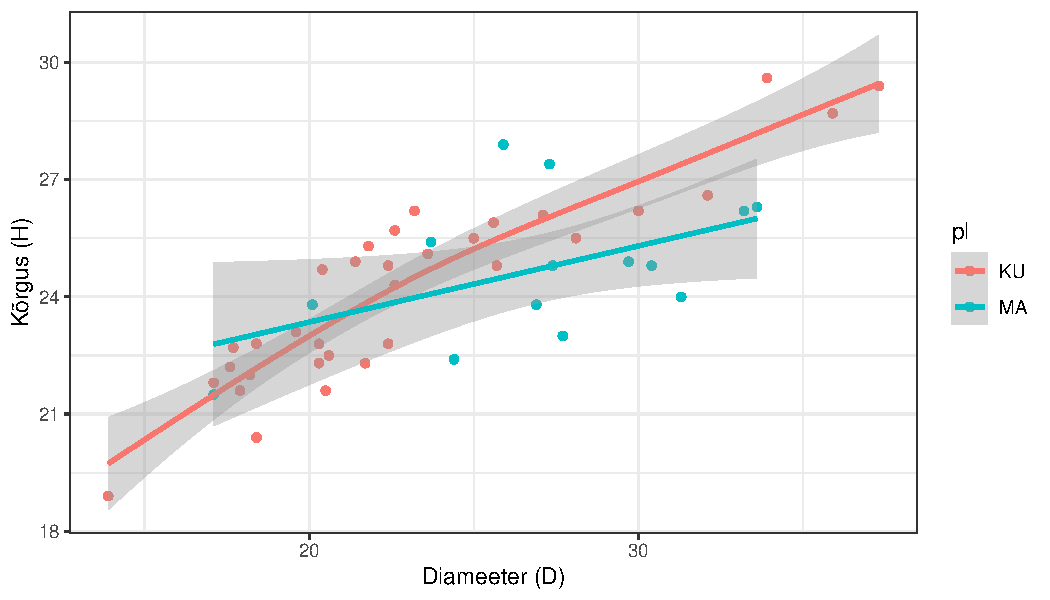
\includegraphics[width=0.8\linewidth]{_main_files/figure-latex/unnamed-chunk-79-1} \caption{Mittelineaarne regressioon}\label{fig:unnamed-chunk-79}
\end{figure}

Kontrollime

\begin{Shaded}
\begin{Highlighting}[]
\FunctionTok{plot}\NormalTok{(}\FunctionTok{fitted}\NormalTok{(mudel), }\FunctionTok{resid}\NormalTok{(mudel),}
 \AttributeTok{xlab =} \StringTok{"Ennustatud väärtused"}\NormalTok{,}
 \AttributeTok{ylab =} \StringTok{"Jäägid"}
\NormalTok{ )}
\FunctionTok{abline}\NormalTok{(}\AttributeTok{h =} \DecValTok{0}\NormalTok{, }\AttributeTok{col =} \StringTok{"red"}\NormalTok{)}
\end{Highlighting}
\end{Shaded}

\begin{figure}[!ht]
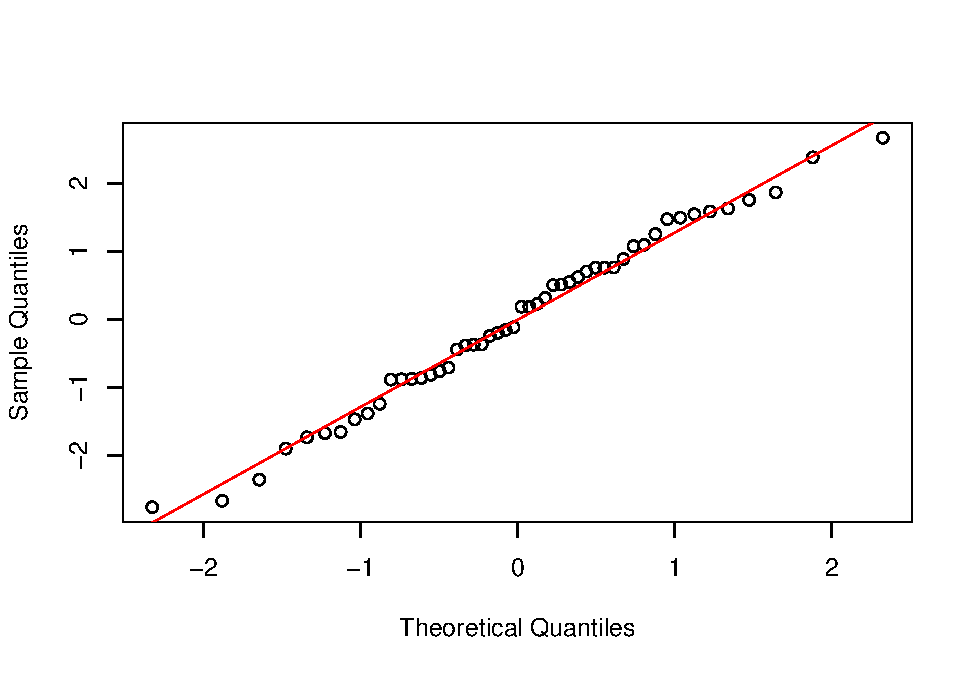
\includegraphics[width=0.8\linewidth]{_main_files/figure-latex/unnamed-chunk-80-1} \caption{Jäägid vs ennustatud}\label{fig:unnamed-chunk-80}
\end{figure}

\begin{Shaded}
\begin{Highlighting}[]
\FunctionTok{qqnorm}\NormalTok{(}\FunctionTok{resid}\NormalTok{(mudel), }\AttributeTok{main =} \StringTok{""}\NormalTok{)}
\FunctionTok{qqline}\NormalTok{(}\FunctionTok{resid}\NormalTok{(mudel), }\AttributeTok{col =} \StringTok{"red"}\NormalTok{)}
\end{Highlighting}
\end{Shaded}

\begin{figure}[!ht]
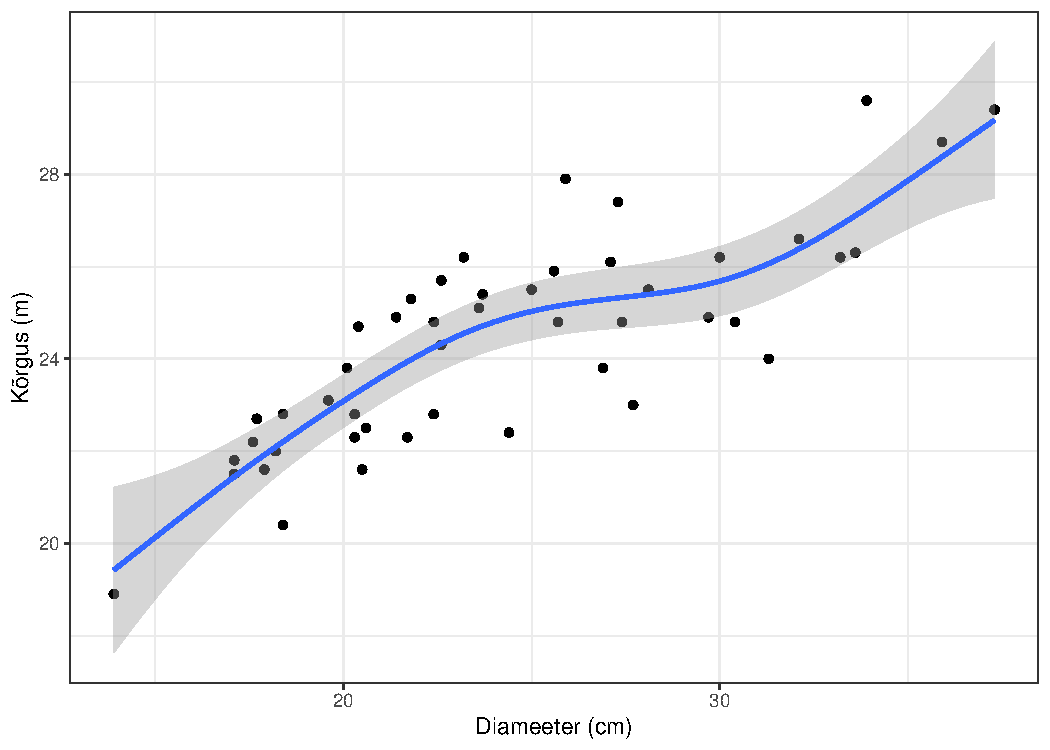
\includegraphics[width=0.8\linewidth]{_main_files/figure-latex/unnamed-chunk-81-1} \caption{Jääkide normaaljaotuse test}\label{fig:unnamed-chunk-81}
\end{figure}

\clearpage

\section{MS Excel}\label{ms-excel-1}

\textbf{Andmete sisestamine.} Avage fail, kus on puude diameetrid ja kõrgused.

\textbf{Algparameetrite väärtuste sisestamine:} Valige kolm vaba lahtrit ja sisestage neisse algparameetrite väärtused a, b ja c jaoks. Need väärtused võivad olla suvalised, aga parema tulemuse saamiseks peaksid need olema lähedased oodatud väärtustele. Näiteks võite alustada a = 20, b = 10 ja c = 3. Nimetage need lahtrid vastavalt ``a'', ``b'' ja ``c''.

\textbf{Arvutatud kõrguse veeru loomine:} Looge uus veerg nimega ``Arvutatud H''. Esimesse lahtrisse sisestage valem: \texttt{=1.3\ +\ \$a\ *\ (\$D2\ /\ (\$D2\ +\ \$b))\^{}\$c}. Asendage \texttt{\$a}, \texttt{\$b} ja \texttt{\$c} vastavate algparameetrite lahtritega (nt \texttt{\$F\$1,}\$F\(2, `\)F\(3`). `\)D2` on esimese diameetri väärtus. See valem arvutab kõrguse vastavalt sisestatud diameetrile ja algparameetrite väärtustele.

\textbf{Valemi kopeerimine:} Lohistage esimese ``Arvutatud H'' lahtri paremas alumises nurgas olevat ruudukest alla, et kopeerida valem kõikidele diameetri väärtustele.

\textbf{Ruutkeskmise vea arvutamine:} Valige vaba lahter ja sisestage valem \texttt{=SUMXMY2(H2:Hn,\ E2:En)/COUNT(H2:Hn)}. See valem arvutab ruutkeskmise vea (RMSE) mõõdetud kõrguse (H) ja arvutatud kõrguse (Arvutatud H) vahel. \texttt{H2:Hn} on mõõdetud kõrguste vahemik ja \texttt{E2:En} on arvutatud kõrguste vahemik.

\textbf{Solveri käivitamine:} Avage menüüst ``Andmed'' -\textgreater{} ``Solver''. Kui Solverit menüüs ei ole, peate selle lisandmoodulitest aktiveerima (Fail -\textgreater{} Suvandid -\textgreater{} Lisandmoodulid -\textgreater{} Exceli lisandmoodulid -\textgreater{} Mine\ldots{} -\textgreater{} Märkige ruut ``Solver Add-in'' ja vajutage ``OK'').

\textbf{Solveri seadistamine:}
* Määrake ``Seadista eesmärk'' lahtriks RMSE lahter.
* Valige ``Min'', et minimeerida RMSE.
* ``Muutuvate lahtrite kaupa'' lahtritesse sisestage algparameetrite a, b ja c lahtrid.
* Vajutage ``Lahenda''.

\textbf{Tulemuste analüüs:} Solver kohandab parameetrite a, b ja c väärtusi, et minimeerida RMSE. Kui Solver on lahenduse leidnud, kuvatakse leitud parameetrite väärtused ja minimaalne RMSE. Nüüd on teil mittelineaarne regressioonimudel, mis kirjeldab puude kõrguse ja diameetri seost teie andmete põhjal.

\textbf{Lisamärkused:}

\begin{itemize}
\tightlist
\item
  Solver ei pruugi alati leida optimaalset lahendust. Proovige erinevaid algparameetrite väärtusi ja käivitage Solver uuesti.
\item
  Saate visualiseerida oma andmeid ja leitud regressioonikõverat, luues hajuvusdiagrammi, kus x-teljel on diameeter ja y-teljel kõrgus. Lisage diagrammile trendijoon, valides ``Kohandatud'' ja sisestades regressioonivõrrandi.
\item
  Hinnake mudeli sobivust, arvestades RMSE väärtust ja visuaalset vastavust andmetele.
\end{itemize}

\chapter{Mitteparameetriline analüüs}\label{mitteparameetriline-analuxfcuxfcs}

\section{Üldistatud aditiivne mudel}\label{uxfcldistatud-aditiivne-mudel}

Üldistatud aditiivne mudel (GAM) on statistiline mudel, mis ühendab lineaarse mudeli omadused aditiivsete funktsioonide abil. Lihtsamalt öeldes on GAM mudel, mis modelleerib funktsioontunnust ühe või mitme argumenttunnuse summa abil, kus iga argumenttunnuse mõju funktsioontunnusele modelleeritakse splainfunktsiooni abil.

Splainfunktsioon on matemaatiline funktsioon, mida kasutatakse andmete interpoleerimiseks ja sujuvaks lähendamiseks. See on ühesuguse struktuuriga tükiti polünomiaalne funktsioon, mis on konstrueeritud nii, et see oleks sujuv ja pidev andmepunktide vahel. See tähendab, et spline funktsioonil ei ole järske hüppeid ega nurki, mis teeb selle ideaalseks tööriistaks sujuvate kõverate ja pindade modelleerimiseks.

Selles näites kasutame R-i paketti \texttt{mgcv} GAM mudeli sobitamiseks. Eesmärk on modelleerida puu kõrguse ja diameetri vahelist seost, eeldades, et see seos ei pruugi olla lineaarne.

Kõigepealt laadime andmestiku, mis sisaldab puude kõrguse ja diameetri mõõtmiste andmeid.

\begin{Shaded}
\begin{Highlighting}[]
\CommentTok{\# Laadime peatükis kasutatavad paketid}
\FunctionTok{library}\NormalTok{(dplyr)}
\FunctionTok{library}\NormalTok{(readxl)}
\FunctionTok{library}\NormalTok{(mgcv)}
\end{Highlighting}
\end{Shaded}

\begin{Shaded}
\begin{Highlighting}[]
\CommentTok{\# Andmete laadimine}
\NormalTok{andmed }\OtherTok{\textless{}{-}} \FunctionTok{read\_excel}\NormalTok{(}\StringTok{"data/naited.xlsx"}\NormalTok{,}\StringTok{"prt\_andmed"}\NormalTok{) }\SpecialCharTok{\%\textgreater{}\%} \FunctionTok{filter}\NormalTok{(h }\SpecialCharTok{\textgreater{}} \DecValTok{0}\NormalTok{)}
\end{Highlighting}
\end{Shaded}

GAM mudeli lähendamiseks kasutame funktsiooni \texttt{gam()} paketist \texttt{mgcv}. Kasutame splainfunktsiooni diameetri muutuja jaoks, et modelleerida mittelineaarset seost.

\begin{Shaded}
\begin{Highlighting}[]
\CommentTok{\# GAM mudeli sobitamine}
\NormalTok{mudel }\OtherTok{\textless{}{-}} \FunctionTok{gam}\NormalTok{(h }\SpecialCharTok{\textasciitilde{}} \FunctionTok{s}\NormalTok{(d), }\AttributeTok{data =}\NormalTok{ andmed)}
\end{Highlighting}
\end{Shaded}

Selles koodis:

\begin{itemize}
\tightlist
\item
  \texttt{H\ \textasciitilde{}\ s(D)} määrab mudeli valemi. \texttt{H} on funktsioontunnus ja \texttt{s(D)} määrab, et diameetri (D) mõju kõrgusele modelleeritakse sujuva funktsiooni \texttt{s()} abil.
\item
  \texttt{data\ =\ andmed} määrab andmestiku, mida kasutada.
\end{itemize}

\textbf{3. Mudeli kokkuvõtte vaatamine:}

Saame mudeli kohta detailse kokkuvõtte funktsiooni \texttt{summary()} abil:

\begin{Shaded}
\begin{Highlighting}[]
\CommentTok{\# Mudeli kokkuvõte}
\FunctionTok{summary}\NormalTok{(mudel)}
\end{Highlighting}
\end{Shaded}

\begin{verbatim}

Family: gaussian 
Link function: identity 

Formula:
h ~ s(d)

Parametric coefficients:
            Estimate Std. Error t value Pr(>|t|)    
(Intercept)   24,368      0,182     134   <2e-16 ***
---
Signif. codes:  0 '***' 0,001 '**' 0,01 '*' 0,05 '.' 0,1 ' ' 1

Approximate significance of smooth terms:
      edf Ref.df  F p-value    
s(d) 3,68   4,61 24  <2e-16 ***
---
Signif. codes:  0 '***' 0,001 '**' 0,01 '*' 0,05 '.' 0,1 ' ' 1

R-sq.(adj) =  0,705   Deviance explained = 72,8%
GCV = 1,7242  Scale est. = 1,5525    n = 47
\end{verbatim}

Kokkuvõte annab meile informatsiooni mudeli sobivuse kohta, sh:

\begin{itemize}
\tightlist
\item
  \textbf{Parametric coefficients:} Kui mudelis on ka lineaarseid komponente, näidatakse siin nende koefitsiendid. Kuna mudelis ühtegi lineaarset tunnust ei ole kasutatud, siis on siin ainult vabaliige \texttt{(Intercept)}.
\item
  \textbf{Approximate significance of smooth terms:} Siin näeme p-väärtuse hinnangut splainfunktsiooni olulisuse kohta. Madal p-väärtus (\textless0.05) viitab statistiliselt olulisele mittelineaarsele seosele diameetri ja kõrguse vahel.
\item
  \textbf{R-sq.(adj):} Korrigeeritud determinatsioonikordaja näitab, kui suure osa kõrguse varieeruvusest mudel seletab.
\item
  \textbf{Deviance explained:} Sarnane determinatsioonikordajale, näitab mudeli poolt seletatud hälbimuse osakaalu.
\end{itemize}

Kasutades funktsiooni \texttt{coef()}, näeme splainfunktsiooni polünoomi parameetrite väärtusi.

\begin{Shaded}
\begin{Highlighting}[]
\FunctionTok{coef}\NormalTok{(mudel)}
\end{Highlighting}
\end{Shaded}

\begin{verbatim}
(Intercept)      s(d).1      s(d).2      s(d).3      s(d).4      s(d).5 
   24,36809    -1,65141    -0,89974    -0,00196     0,03456    -0,04304 
     s(d).6      s(d).7      s(d).8      s(d).9 
    0,18773    -0,13235    -0,81294     3,44774 
\end{verbatim}

Saame visualiseerida diameetri ja kõrguse vahelist seost funktsiooni \texttt{plot()} abil:

\begin{Shaded}
\begin{Highlighting}[]
\CommentTok{\# Mudeli visualiseerimine}
\FunctionTok{par}\NormalTok{(}\AttributeTok{mar=}\FunctionTok{c}\NormalTok{(}\DecValTok{4}\NormalTok{,}\DecValTok{4}\NormalTok{,}\DecValTok{1}\NormalTok{,}\DecValTok{1}\NormalTok{), }\AttributeTok{mgp=}\FunctionTok{c}\NormalTok{(}\DecValTok{2}\NormalTok{, }\FloatTok{0.7}\NormalTok{, }\DecValTok{0}\NormalTok{))}
\FunctionTok{plot}\NormalTok{(mudel)}
\end{Highlighting}
\end{Shaded}

\begin{figure}[!ht]
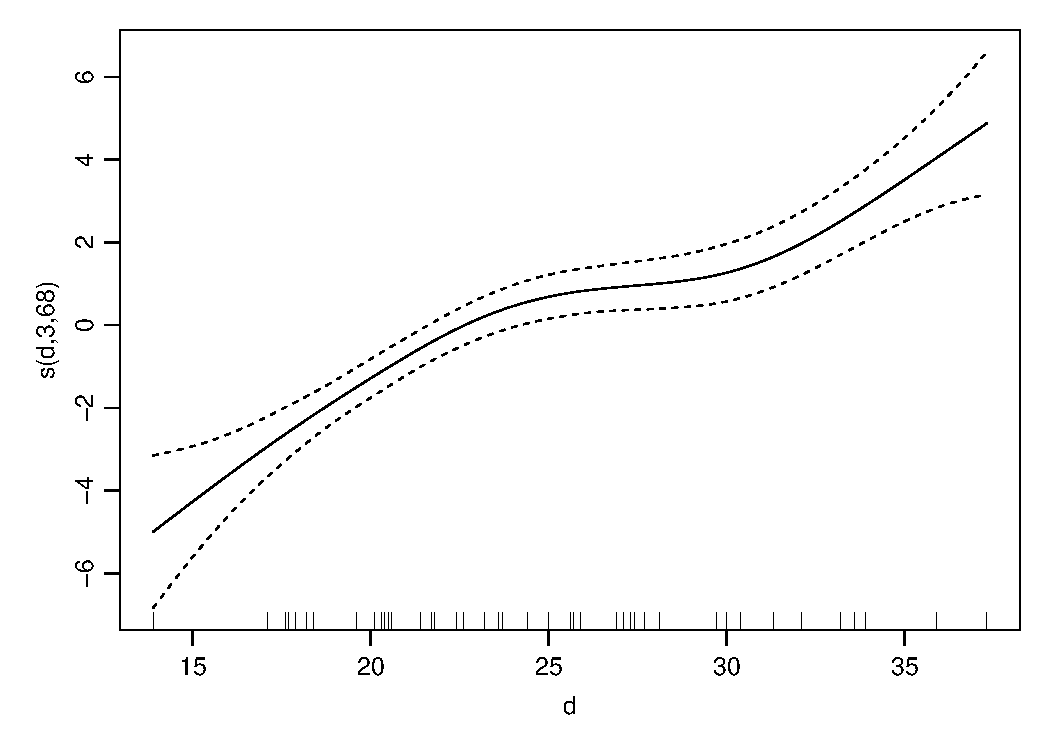
\includegraphics[width=0.8\linewidth]{_main_files/figure-latex/unnamed-chunk-88-1} \caption{Kõrguse sõltuvus diameetrist}\label{fig:unnamed-chunk-88}
\end{figure}

See kuvab graafiku, mis näitab diameetri mõju puu kõrgusele. Pidevjoon näitab modelleeritud seost ja kriipsjooned näitavad usaldusvahemikku. See graafik aitab visuaalselt hinnata seose kuju ja mittelineaarsust.

Saame kasutada mudelit uute puude kõrguse ennustamiseks, andes ette diameetri väärtused funktsiooni \texttt{predict()} abil:

\begin{Shaded}
\begin{Highlighting}[]
\CommentTok{\# Uute diameetrite väärtused}
\NormalTok{uued\_diameetrid }\OtherTok{\textless{}{-}} \FunctionTok{data.frame}\NormalTok{(}\AttributeTok{d =} \FunctionTok{c}\NormalTok{(}\DecValTok{12}\NormalTok{, }\DecValTok{22}\NormalTok{, }\DecValTok{32}\NormalTok{))}

\CommentTok{\# Ennustuste tegemine}
\NormalTok{ennustused }\OtherTok{\textless{}{-}} \FunctionTok{predict}\NormalTok{(mudel, }\AttributeTok{newdata =}\NormalTok{ uued\_diameetrid)}

\CommentTok{\# Ennustuste kuvamine}
\FunctionTok{print}\NormalTok{(ennustused)}
\end{Highlighting}
\end{Shaded}

\begin{verbatim}
   1    2    3 
18,1 24,1 26,3 
\end{verbatim}

\section{\texorpdfstring{Visualiseerimine paketiga \texttt{ggplot2}}{Visualiseerimine paketiga ggplot2}}\label{visualiseerimine-paketiga-ggplot2}

Oletame, et meil on samad andmed puude kõrguse (h) ja diameetri (d) kohta nagu eelmistes näidetes, aga me tahame luua hajuvusdiagrammi ja lisada sellele sujuva joone otse \texttt{ggplot2} abil, ilma et peaks eraldi \texttt{gam()} funktsiooni kasutama.

\begin{Shaded}
\begin{Highlighting}[]
\CommentTok{\# Laadi pakett}
\FunctionTok{library}\NormalTok{(ggplot2)}
\end{Highlighting}
\end{Shaded}

Kasutame \texttt{ggplot()} funktsiooni koos \texttt{geom\_point()} ja \texttt{geom\_smooth()} funktsioonidega:

\begin{Shaded}
\begin{Highlighting}[]
\FunctionTok{ggplot}\NormalTok{(andmed, }\FunctionTok{aes}\NormalTok{(}\AttributeTok{x =}\NormalTok{ d, }\AttributeTok{y =}\NormalTok{ h)) }\SpecialCharTok{+}
  \FunctionTok{geom\_point}\NormalTok{() }\SpecialCharTok{+}  \CommentTok{\# Joonistab hajuvusdiagrammi}
  \FunctionTok{geom\_smooth}\NormalTok{(}\AttributeTok{method =} \StringTok{"gam"}\NormalTok{, }\AttributeTok{formula =}\NormalTok{ y }\SpecialCharTok{\textasciitilde{}} \FunctionTok{s}\NormalTok{(x)) }\SpecialCharTok{+}  \CommentTok{\# Lisab sujuva joone GAM mudeli abil}
  \FunctionTok{labs}\NormalTok{(}\AttributeTok{x =} \StringTok{"Diameeter (cm)"}\NormalTok{, }\AttributeTok{y =} \StringTok{"Kõrgus (m)"}\NormalTok{) }\SpecialCharTok{+}
  \FunctionTok{theme\_bw}\NormalTok{()}
\end{Highlighting}
\end{Shaded}

\begin{figure}[!ht]
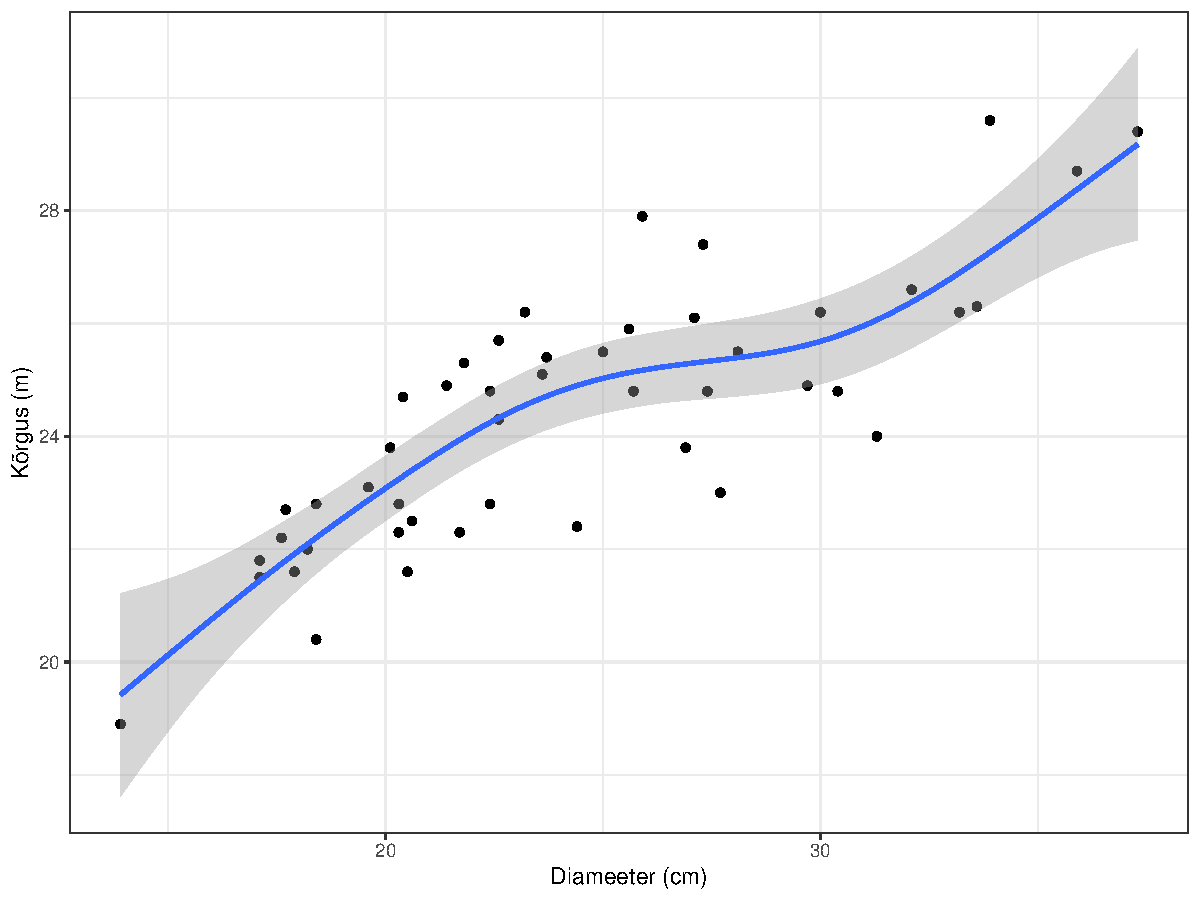
\includegraphics[width=0.8\linewidth]{_main_files/figure-latex/unnamed-chunk-91-1} \caption{Kõrguse sõltuvus diameetrist}\label{fig:unnamed-chunk-91}
\end{figure}

Selgitus:

\begin{itemize}
\tightlist
\item
  \texttt{ggplot(puud,\ aes(x\ =\ d,\ y\ =\ h))}: See rida loob \texttt{ggplot} objekti ja määrab andmestiku (\texttt{andmed}) ning x-telje (diameeter - \texttt{D}) ja y-telje (kõrgus - \texttt{H}) muutujad.
\item
  \texttt{geom\_point()}: See funktsioon lisab graafikule punktid, luues hajuvusdiagrammi. Iga punkt esindab ühte puud.
\item
  \texttt{geom\_smooth(method\ =\ "gam",\ formula\ =\ y\ \textasciitilde{}\ s(x))}: See funktsioon lisab graafikule sujuva joone.

  \begin{itemize}
  \tightlist
  \item
    \texttt{method\ =\ "gam"}: Määrab, et sujuva joone sobitamiseks kasutatakse GAM mudelit.
  \item
    \texttt{formula\ =\ y\ \textasciitilde{}\ s(x)}: Määrab mudeli valemi. \texttt{y\ \textasciitilde{}\ s(x)} tähendab, et \texttt{y} (meie puhul kõrgus \texttt{H}) modelleeritakse \texttt{x} (meie puhul diameeter \texttt{D}) sujuva funktsiooni \texttt{s()} abil. See on sama valem, mida kasutasime eelmistes näidetes \texttt{gam()} funktsiooni sees.
  \end{itemize}
\item
  \texttt{labs(...)}: Määrab telgede sildid ja graafiku pealkirja.
\item
  \texttt{theme\_bw()}: Muudab graafiku teema must-valgeks.
\end{itemize}

Sarnaselt eelmisele näitele saate \texttt{ggplot2} abil graafikut vastavalt oma soovile kohandada. Näiteks:

\begin{Shaded}
\begin{Highlighting}[]
\FunctionTok{ggplot}\NormalTok{(andmed, }\FunctionTok{aes}\NormalTok{(}\AttributeTok{x =}\NormalTok{ d, }\AttributeTok{y =}\NormalTok{ h, }\AttributeTok{color =}\NormalTok{ pl)) }\SpecialCharTok{+}
  \CommentTok{\# Muudab punktide värvi, kuju ja suurust}
  \FunctionTok{geom\_point}\NormalTok{() }\SpecialCharTok{+}  
  \CommentTok{\# Eemaldab usaldusvahemiku ja muudab joone värvi}
  \FunctionTok{geom\_smooth}\NormalTok{(}\AttributeTok{method =} \StringTok{"gam"}\NormalTok{, }\AttributeTok{formula =}\NormalTok{ y }\SpecialCharTok{\textasciitilde{}} \FunctionTok{s}\NormalTok{(x)) }\SpecialCharTok{+}  
  \FunctionTok{labs}\NormalTok{(}\AttributeTok{x =} \StringTok{"Diameeter (D)"}\NormalTok{, }\AttributeTok{y =} \StringTok{"Kõrgus (H)"}\NormalTok{) }\SpecialCharTok{+}
  \FunctionTok{theme\_bw}\NormalTok{()}
\end{Highlighting}
\end{Shaded}

\begin{figure}[!ht]
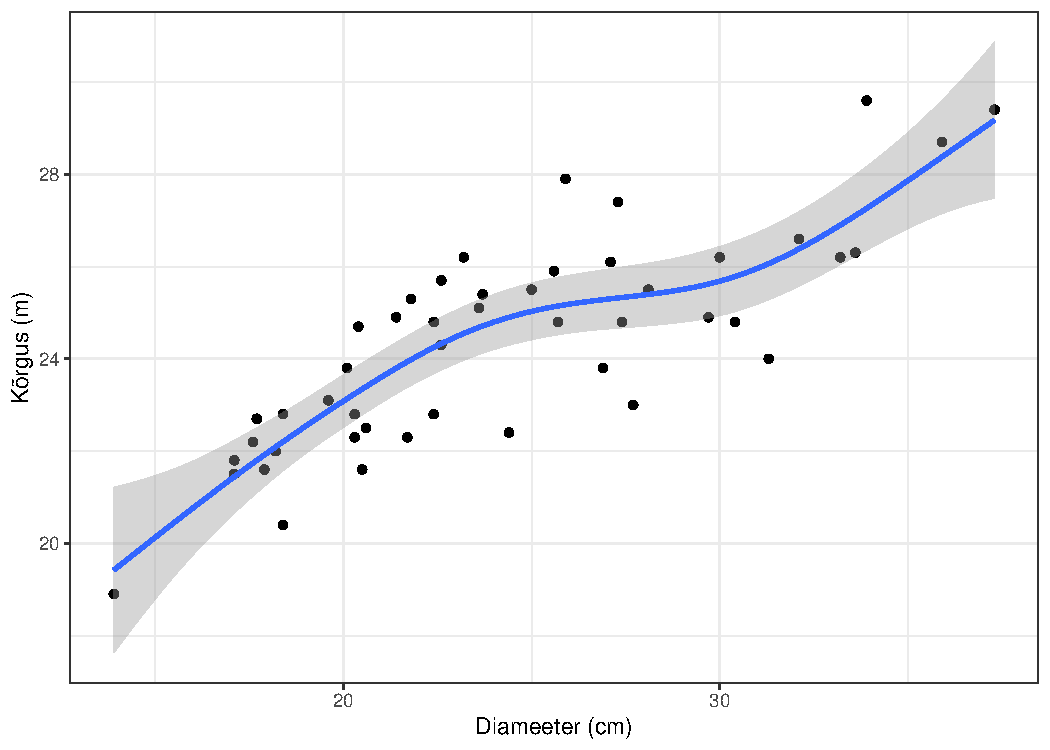
\includegraphics[width=0.8\linewidth]{_main_files/figure-latex/unnamed-chunk-92-1} \caption{Kõrguse sõltuvus diameetrist}\label{fig:unnamed-chunk-92}
\end{figure}

Selles näites:

\begin{itemize}
\tightlist
\item
  \texttt{aes(x\ =\ D,\ y\ =\ H,\ color\ =\ PL)} on lisatud, et värv sõltub puuliigist.
\end{itemize}

See näide demonstreerib, kuidas luua hajuvusdiagramm ja lisada sellele sujuv joon, mis on sobitatud GAM mudeli abil, kasutades ainult \texttt{ggplot2} funktsioone. See on mugav viis kiiresti visualiseerida mittelineaarseid seoseid andmetes ilma eraldi GAM mudelit sobitamata. \texttt{ggplot2} pakub laialdasi võimalusi graafikute kohandamiseks, võimaldades luua informatiivseid ja visuaalselt meeldivaid visualiseeringuid.

\bibliography{book.bib,packages.bib}

\end{document}
